\documentclass[11pt,a4paper]{jsarticle}

\usepackage[dvipdfmx]{graphicx}
\usepackage{graphicx}
\usepackage[top=20truemm,bottom=20truemm,left=25truemm,right=25truemm]{geometry}
\usepackage{comment}

\title{卒業研究前期報告書}
\author{東京大学工学部物理工学科 賀川研究室 平松信義}
\date{\today}
\begin{document}
\maketitle

\tableofcontents
\newpage

\section{はじめに}
%相転移/急冷/超伝導/鉄鋼/強相関電子系/準定常状態の電流励起/電荷秩序と競合した超伝導相
%なぜ秩序相の研究に価値があるのか読者任せになっている
%なぜIrTeを研究するのか: 非定常的な超伝導体ー絶縁体転移が知られているから
%顕微鏡構築と抵抗測定
%この系はスピン- 軌道相互作用の効果が大きく、非従来型の超伝導が予想されている。
超伝導はある臨界温度以下で電気抵抗がゼロになる現象で、1911年にオランダのオンネスにより発見された。多彩かつ応用上有利な性質を超伝導物質は示すため、現在まで様々な超伝導物質に関して活発な研究開発が進められてきた。特に1986年に銅酸化物高温超伝導体が発見されて以来、銅酸化物を含む強相関電子系と呼ばれる物質群は精力的な研究の対象となった。

銅酸化物超伝導体は、母物質に少量の不純物を添加・元素置換したとき超伝導が発現する。この超伝導は電子間の相対的に強い反発力により引き起こされるもので、電荷やスピンなどの秩序化と起源を同じくしている。これらの超伝導相と秩序相は起源を同じくするため、一方の理解は他方の理解にも繋がる。またこの二つの相の競合は避けられない。近年、ある銅酸化物の秩序相に赤外光パルスを入射すると、過渡的に、超伝導相への転移が起こることが示された\cite{Fausti}。
IrTe$_2$は低温で電荷が一次元的に配列する電荷秩序状態となる(電荷密度波)が、この物質にパラジウム(Pd)やプラチナ(Pt)を添加すると臨界温度3Kで超伝導を示す。\cite{}近年、薄膜のIrTe$_2$に現れる電荷秩序を電流パルス印加後に急冷し破壊すると、競合する超伝導状態が現れることが実験により示された\cite{SC_IrTe2}。

しかしこのような急冷後に現れる超伝導相に関しては、いまだ理解されていないことが多い。本研究の目的はIrTe$_2$の超伝導状態をパルス光を用いても誘起できることを示し、その超伝導状態が実現される過程の理解を深めることである。筆者は2018年前期の実験において、偏光顕微鏡を用いてIrTe$_2$バルク試料の電荷秩序相を観察して、その理解を深めることを目標にした。まず偏光顕微光学系の設計と構築を行った。そして光学クライオスタット内の試料の抵抗を測定しながら温度を変化させ、偏光顕微鏡によって試料を観察した。本報告書では実験によって得られた成果と今後の課題について報告する。

\section{実験方法}
IrTe$_2$試料は理化学研究所の上谷研究員から提供を受けた。厚さ0.2mm、高さ0.7mm、幅1.3mm程度のバルク試料に二つの電圧端子と二つの電流端子を接続し、試料の抵抗を四端子法を用いて測定した。
試料は光学クライオスタット内に格納し、試料の温度をヘリウム冷凍機とヒーターを用いて制御した。
\begin{figure}[p]
  \begin{center}
   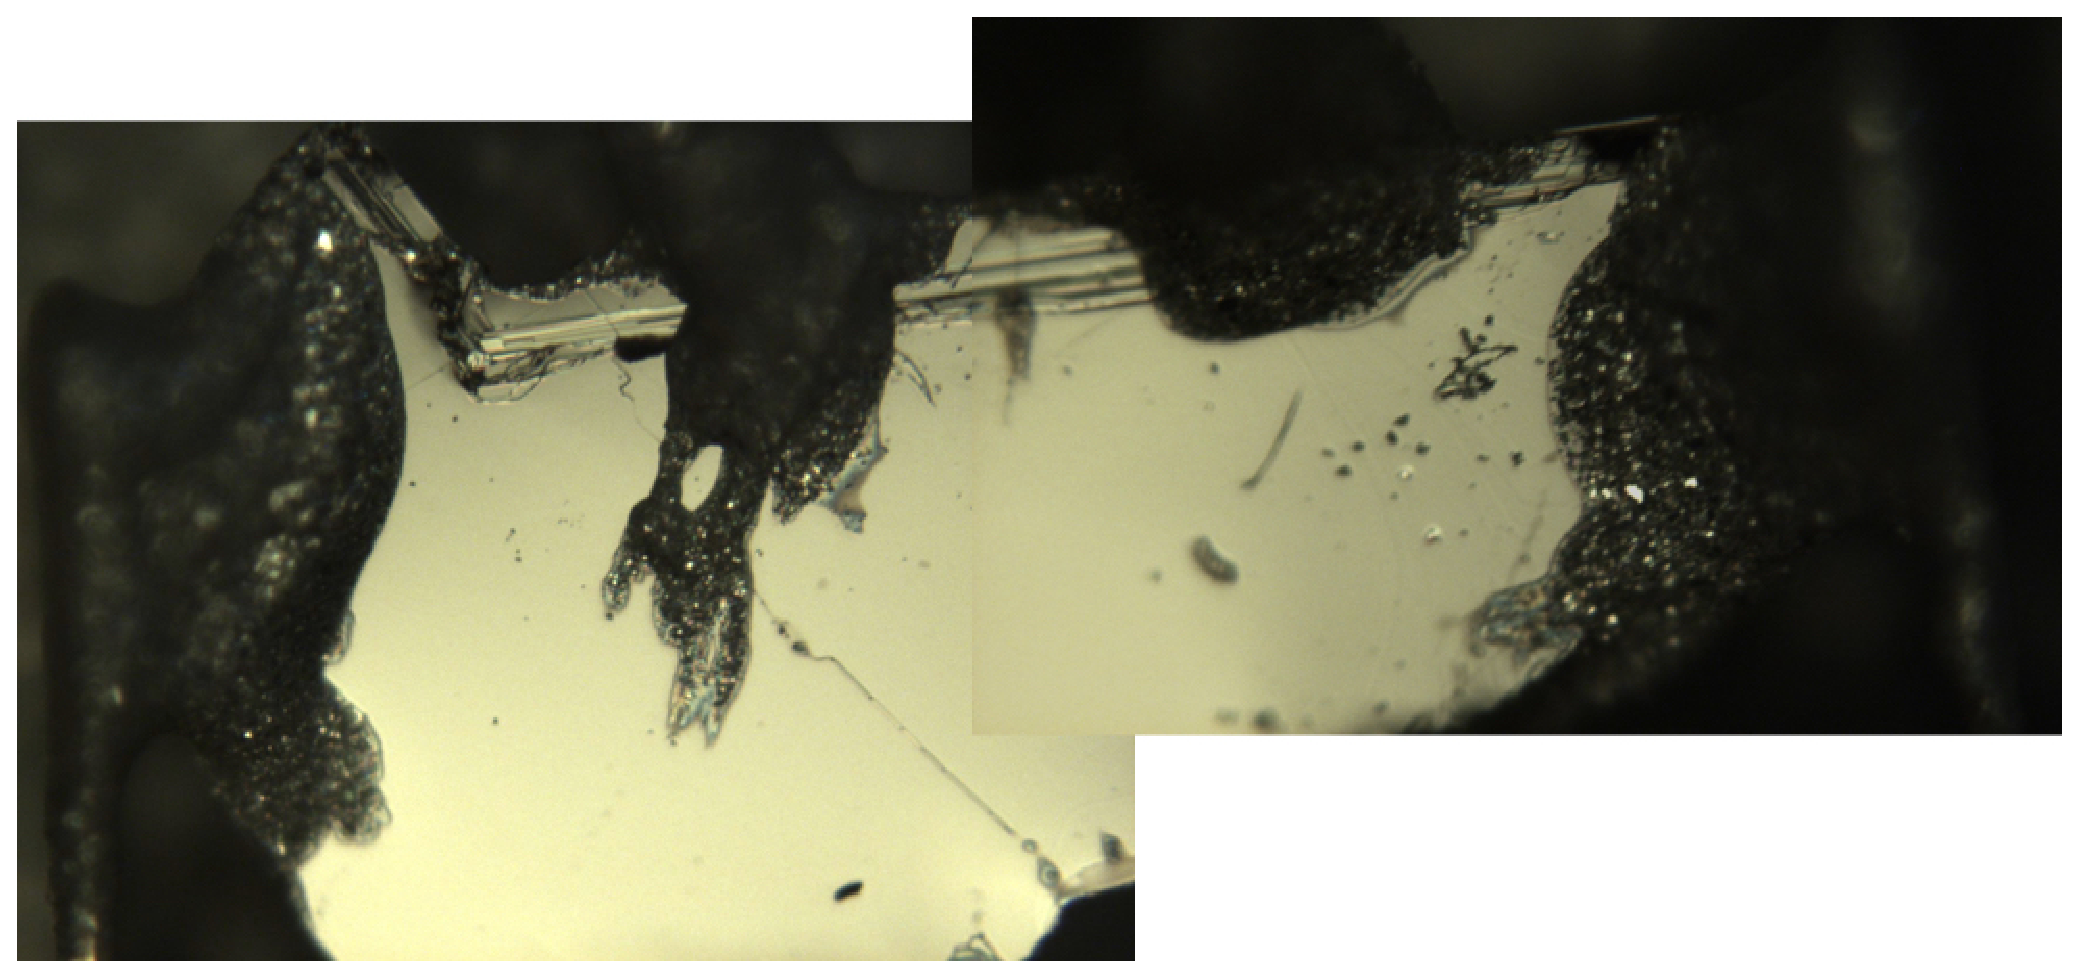
\includegraphics[width=100mm]{sample.eps}
  \end{center}
  \caption{試料の外観}
  \label{fig:sample}
\end{figure}

\subsection{四端子法}
試料に四端子を接続する時の注意点を\ref{sec:4terminal}に書き記す。 四端子を取り付けた後の試料の外観を図\ref{fig:sample}に示した。なお抵抗測定の際にロックインアンプを用いることで信号のSN比を高めた。ロックインアンプの周波数は77Hz、積分時間は1秒にとった。

\subsection{偏光顕微光学系}
試料表面の構造を観察するために、反射配置の偏光顕微鏡を構築した。光学系の模式図を図\ref{fig:microscope}に示す。光学素子は光源とコリメータを除き、全てXYZステージの上に固定し、位置を調整できるようにした。白熱ランプ(Edmund製\#MI-150)の赤外域をフィルタでカットした後、ファイバーを通しコリメータ(Edmund製\#LENS ASP0.15)に導き平行光に直した。さらにその平行光を中心波長532nm、半値全幅3nmのバンドパスフィルタ(Thorlabs製\#FL-532-3)に通し、拡散角度$1^\circ$のホログラフィックディフューザー(Edmund製\#47-991)で拡散した。ここでホログラフィックディフューザーを用いたのは、平行光の空間的なコヒーレンスを小さくして照明光に向いたものにするためである。そして消光比15000程度のガラス偏光フィルター(Edmund製\#43-786)を透過させて入射光の偏光を制御し、無偏光ビームスプリッタ(Thorlabs製\#BSW41-532)と対物レンズ(Mitsutoyo製M Plan Apoシリーズ/倍率x10)を通して試料に入射した。ここでビームスプリッタは透過率と反射率がともに偏光状態に依存せず、波長532nm程度で50\%程度となる素子を選定した。試料からの反射光はビームスプリッタで反射され、検光子を通してCCD上に結像するように調整した。光源の後ろとCCDカメラの前にそれぞれ偏光子と検光子としてグラス偏光フィルタを配置し、独立に回転させることで様々な偏光状態に関する偏光顕微鏡像をとった。
\begin{figure}[p]
  \begin{center}
   \includegraphics[width=100mm,angle=270]{microscope.eps}
  \end{center}
  \caption{偏光顕微光学系の模式図}
  \label{fig:microscope}
\end{figure}


\section{実験結果}
%コントラスト:明るさの違い
%パターン
%領域:ドメイン
%反射率:信号強度
\subsection{300Kと250Kの偏光顕微鏡像の比較}
まず等方的な高温相と異方的な電荷秩序相(低温相)を比較するために、試料の温度を300Kから250Kまでレート1K/minで冷却したあと、同一のレートで250Kから300Kまで加熱した。図\ref{fig:resistance250-300}に温度と抵抗のヒステリシス曲線を示す。冷却時は温度280K付近で不連続に抵抗が増加し、加熱時は温度290K付近で不連続に抵抗が減少した。

図\ref{fig:nonpol300}-\ref{fig:vh300_subtractedby_hv300}は300Kで撮影した顕微鏡写真で、図\ref{fig:nonpol250}-\ref{fig:vh250_subtractedby_hv250}は250Kでの顕微鏡写真である。それぞれ同一の領域を同じ倍率で撮影した。(光源の明るさとCCDの動作条件に関しては後述する。)

まず図\ref{fig:microscope}の顕微光学系から偏光子と検光子を取り外して、無偏光で300Kと250Kの試料の顕微鏡写真をとったものを図\ref{fig:nonpol300}と図\ref{fig:nonpol250}にそれぞれ示す。光源の明るさとCCDの動作条件はそれぞれの画像に関して最適化してある。図\ref{fig:nonpol300}中の青色のスケールバーは、長さ$50 \mu m$を意味する。250Kの図\ref{fig:nonpol250}の試料に関して、画像から反射率が大きい(明るい)領域と反射率が小さい(暗い)領域の存在が明瞭に観察できる。すなわち明暗のコントラスト(反射率の大きい領域と小さい領域の信号強度の相対的な差と定義する)が存在する。明るい領域は、典型的に細長い形をしており、概ね$10 \mu m$オーダーの大きさを持つ。また明るい領域と暗い領域の境界が伸びている方向は三方向あり、画像の横方向となす角度が49度と111度と172度だった。お互いに概ね60度の角度をなしていることが分かる。250Kの無偏光な顕微鏡像(図\ref{fig:nonpol250})に関して、図\ref{fig:nonpol250_profile}左のように黄色のバーに沿って信号強度のプロファイルを取ったものを図\ref{fig:nonpol250_profile}右図に示す。明るい領域と暗い領域でそれぞれ一様な信号強度を持ち、それらの境界で信号強度が急峻に変化するふるまいが確認できた。反射率の相対的な差(コントラスト)は13\%程度と見積もった。図\ref{fig:nonpol250}で観察されたような明暗のコントラストは、300Kの図\ref{fig:nonpol300}の試料では確認できない。

次に、偏光子と検光子を導入した図\ref{fig:microscope}の偏光顕微光学系において、偏光子と検光子の偏光軸を平行に配置した平行偏光の条件で、対応する領域を撮影した。ここで偏光軸の方向は試料の向きを基準にして、図\ref{fig:xy}に示すようにx方向(水平方向)とy方向(鉛直方向)の二つをとった。画像横方向に対してx方向は50度の角をなし、y方向は140度の角をなす。300Kでx方向に偏光子と検光子を調整した顕微鏡像を図\ref{fig:hh300}に示し、y方向に偏光子と検光子を調整した像を図\ref{fig:vv300}にそれぞれ示した。光源の明るさとCCDの動作条件は図\ref{fig:hh300}と図\ref{fig:vv300}で同一である。図\ref{fig:hh300}と図\ref{fig:vv300}を比較しても、強度の違いを除き定性的な違いは見られない。
同様に250Kでx方向の平行偏光とy方向の平行偏光の条件で撮影し、顕微鏡像を図\ref{fig:hh250}と図\ref{fig:vv250}にそれぞれ示した。光源の明るさとCCDの動作条件は図\ref{fig:hh250}と図\ref{fig:vv250}で同一である。無偏光の図\ref{fig:nonpol250}と同様な明暗のパターンが、図\ref{fig:hh250}と図\ref{fig:vv250}に見て取れる。%図\ref{fig:hh250}と図\ref{fig:vv250}を比較すると、対応した領域でも、細長く明るい領域が走る方向によって、反射率に差が見られる。例えば図\ref{fig:vv250}の左下と真ん中の領域で時計の11時-5時の方向(画像横方向に対して111度)に伸びる明るい領域は、図\ref{fig:hh250}の対応する領域に比べて、周囲との明暗のコントラストが比較的小さい。

次に偏光子と検光子の偏光軸を直交させた直交偏光の条件で顕微鏡像を撮影した。300Kでy方向の偏光子とx方向の検光子を調整した顕微鏡像を図\ref{fig:vh300}に示し、x方向の偏光子とy方向の検光子を調整した顕微鏡像を図\ref{fig:hv300}に示した。同様に温度250Kでy方向の偏光とx方向の検光に調整した顕微鏡像を図\ref{fig:vh250}に示し、x方向の偏光とy方向の検光に調整した顕微鏡像を図\ref{fig:hv250}に示した。光源の明るさとCCDの動作条件は、図\ref{fig:vh300}と図\ref{fig:hv300}が同一で、図\ref{fig:hv250}と図\ref{fig:vh250}が同一である。ただしCCDのシャッタースピードを図\ref{fig:vh300}は図\ref{fig:vh250}に比べて遅くしてある(感度: 図\ref{fig:vh300}$=図\ref{fig:hv300}>$図\ref{fig:vh250}=\ref{fig:hv250})。無偏光の図\ref{fig:nonpol250}と同様な明暗のパターンが、図\ref{fig:vh250}と図\ref{fig:vh250}に見て取れる。

300Kの図\ref{fig:vh300}と250Kの図\ref{fig:vh250}を比較すると、感度は300Kの図\ref{fig:vh300}の方が高いにも関わらず、図\ref{fig:vh250}で明るい領域は図\ref{fig:vh300}の対応する領域に比べて明るい。図\ref{fig:hv300}と図\ref{fig:hv250}の比較でも同様なことが言える。すなわち直交偏光の条件で250Kの明るい領域は、周囲と比べて明るいだけでなく300Kの対応する領域に対しても明るい。

図\ref{fig:vh250}と図\ref{fig:hv250}を比較すると、細長く明るい領域が伸びる方向に依存して、対応する領域であっても周囲との明暗のコントラストに差がある。例えば図\ref{fig:vh250}の左下で時計の11時-5時の方向(画像横方向に対して111度)に伸びる領域は、図\ref{fig:hv250}の対応する領域に対して周囲とのコントラストが比較的大きい。一方で、図\ref{fig:vh250}の右上で2時-8時方向(画像横方向に対して49度)に伸びる明るい領域と図\ref{fig:hv250}の対応する領域でコントラストを比較しても差が見られない。すなわち明るく細長い領域が伸びる方向と偏光条件によって、コントラストに差が現れる。このコントラストの差をあらわに見るために図\ref{fig:vh250} と図\ref{fig:hv250}の差分をとった画像を図\ref{fig:vh250_subtractedby_hv250}に示す。図\ref{fig:vh250_subtractedby_hv250}左下で11時-5時方向(画像横方向に対して111度)に伸びる領域でコントラストの差が大きく、右上で2時-8時方向(画像横方向に対して49度)に伸びる領域でコントラストの差が小さいことが確認できる。図\ref{fig:vh250_subtractedby_hv250}と同様に、300Kで直交偏光の図\ref{fig:vh300} と図\ref{fig:hv300}の差分をとった画像を図\ref{fig:vh300_subtractedby_hv300}に示す。図\ref{fig:vh300_subtractedby_hv300}では、250Kの図\ref{fig:vh250_subtractedby_hv250}のような明暗のパターンは現れない。

最後に本節で得られた結果をまとめる。
\begin{enumerate}
\item 300Kから250Kまでレート1K/minで冷却してゆくと、300Kの顕微鏡写真に見られなかった明暗のパターンが、250Kの顕微鏡写真に現れた。その明暗のパターンは無偏光の条件(図\ref{fig:nonpol250})と平行偏光偏光条件(図\ref{fig:hh250}、\ref{fig:vv250})、直交偏光条件(図\ref{fig:vh250}、\ref{fig:hv250})の全条件に関して見て取れる。ただしコントラストは条件により異なる。
\item 明るい領域は、典型的に細長い形をしており、概ね$10 \mu m$オーダーの大きさを持つ。また明るい領域と暗い領域の境界の方向は三方向あり、お互いに概ね60度の角度をなしている。
\item 明るい領域と暗い領域の境界で信号強度は急峻に変化した。無偏光の条件で明るい領域と暗い領域のコントラストは13\%程度である(図\ref{fig:nonpol250_profile})
\item 直交偏光の条件で250Kの明るい領域は、周囲と比べて明るいだけでなく300Kの対応する領域に対しても明るい(図\ref{fig:vh300}、\ref{fig:vh250})
\item 直交偏光の条件で、明るく細長い領域が伸びる方向と偏光/検光方向に依存して周囲との明暗のコントラストが異なる(図\ref{fig:vh250} 、\ref{fig:hv250})
 \end{enumerate}

\begin{figure}[p]
  \begin{minipage}{0.7\hsize}
    \begin{center}
   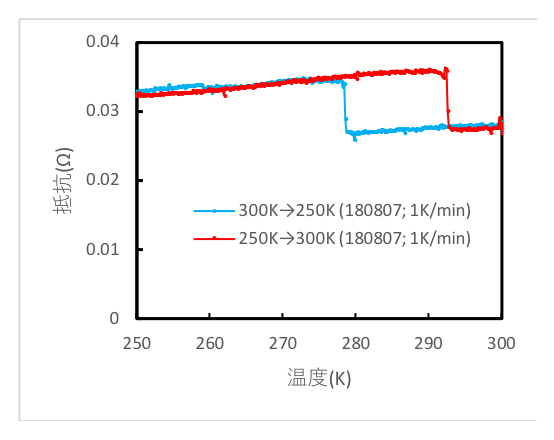
\includegraphics[width=100mm]{resistance250-300.eps}
  \end{center}
  \caption{抵抗の温度依存性}
  \label{fig:resistance250-300}
   \end{minipage}
 \begin{minipage}{0.3\hsize}
  \begin{center}
   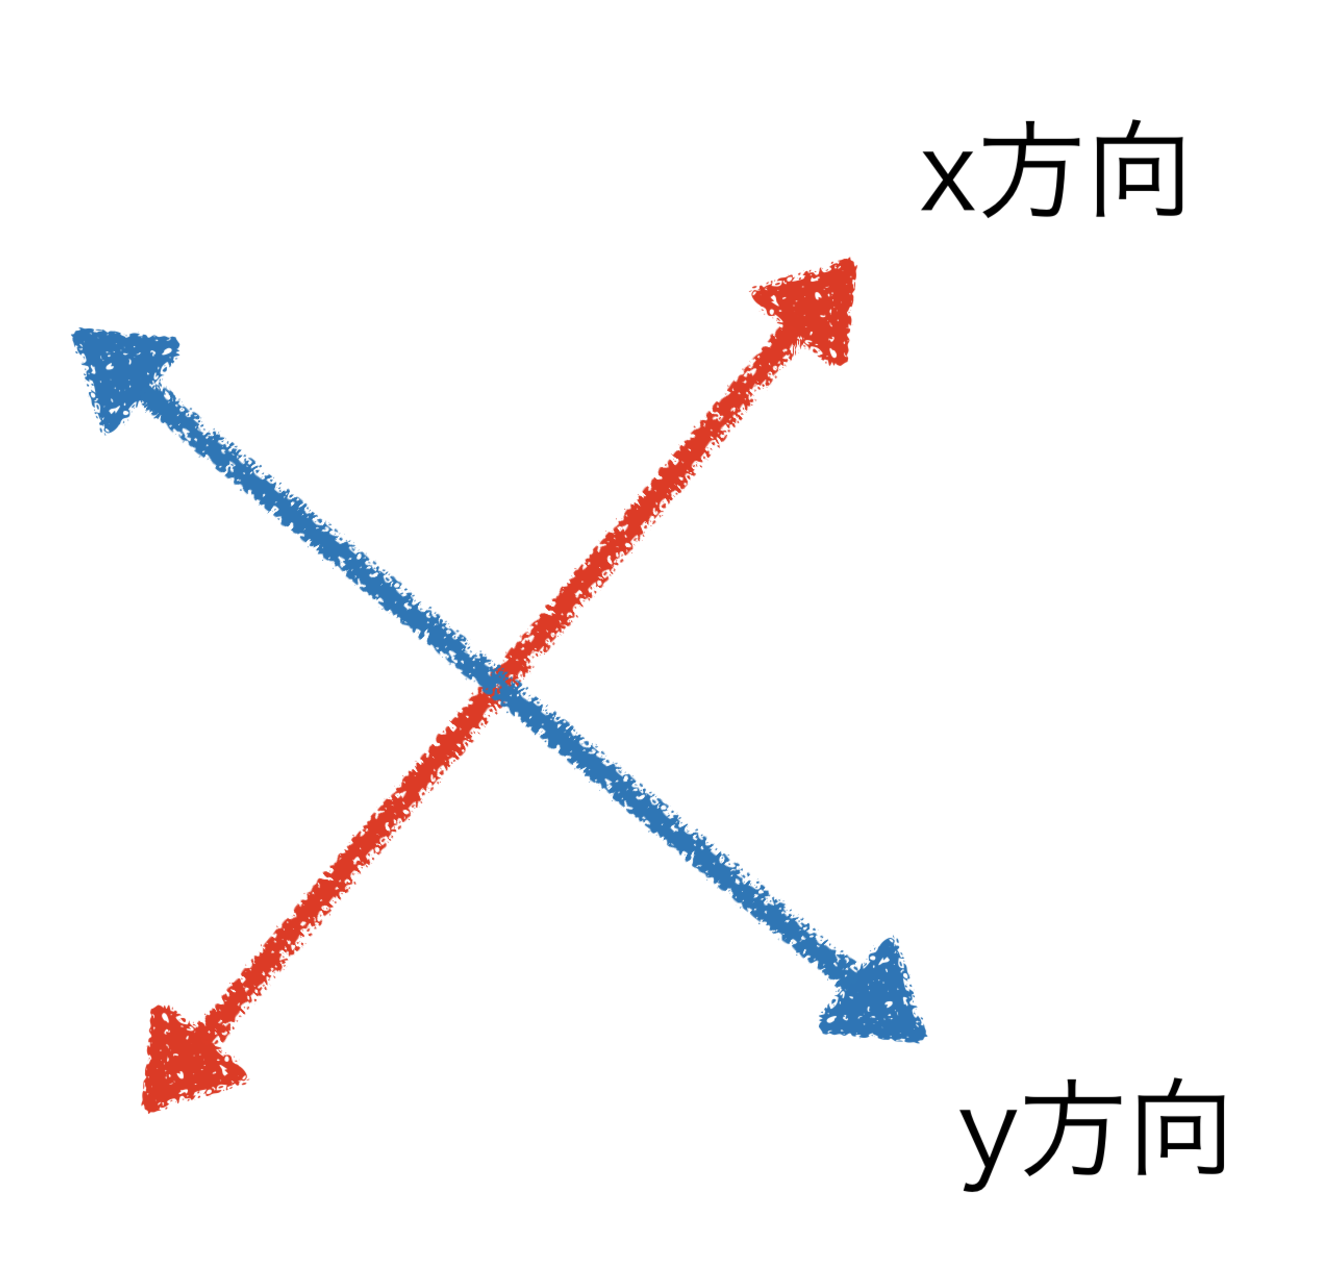
\includegraphics[width=50mm]{xy.eps}
  \end{center}
  \caption{偏光のx方向とy方向}
  \label{fig:xy}
  \end{minipage}
\end{figure}

\begin{figure}[p]
 \begin{minipage}{0.333\hsize}
  \begin{center}
   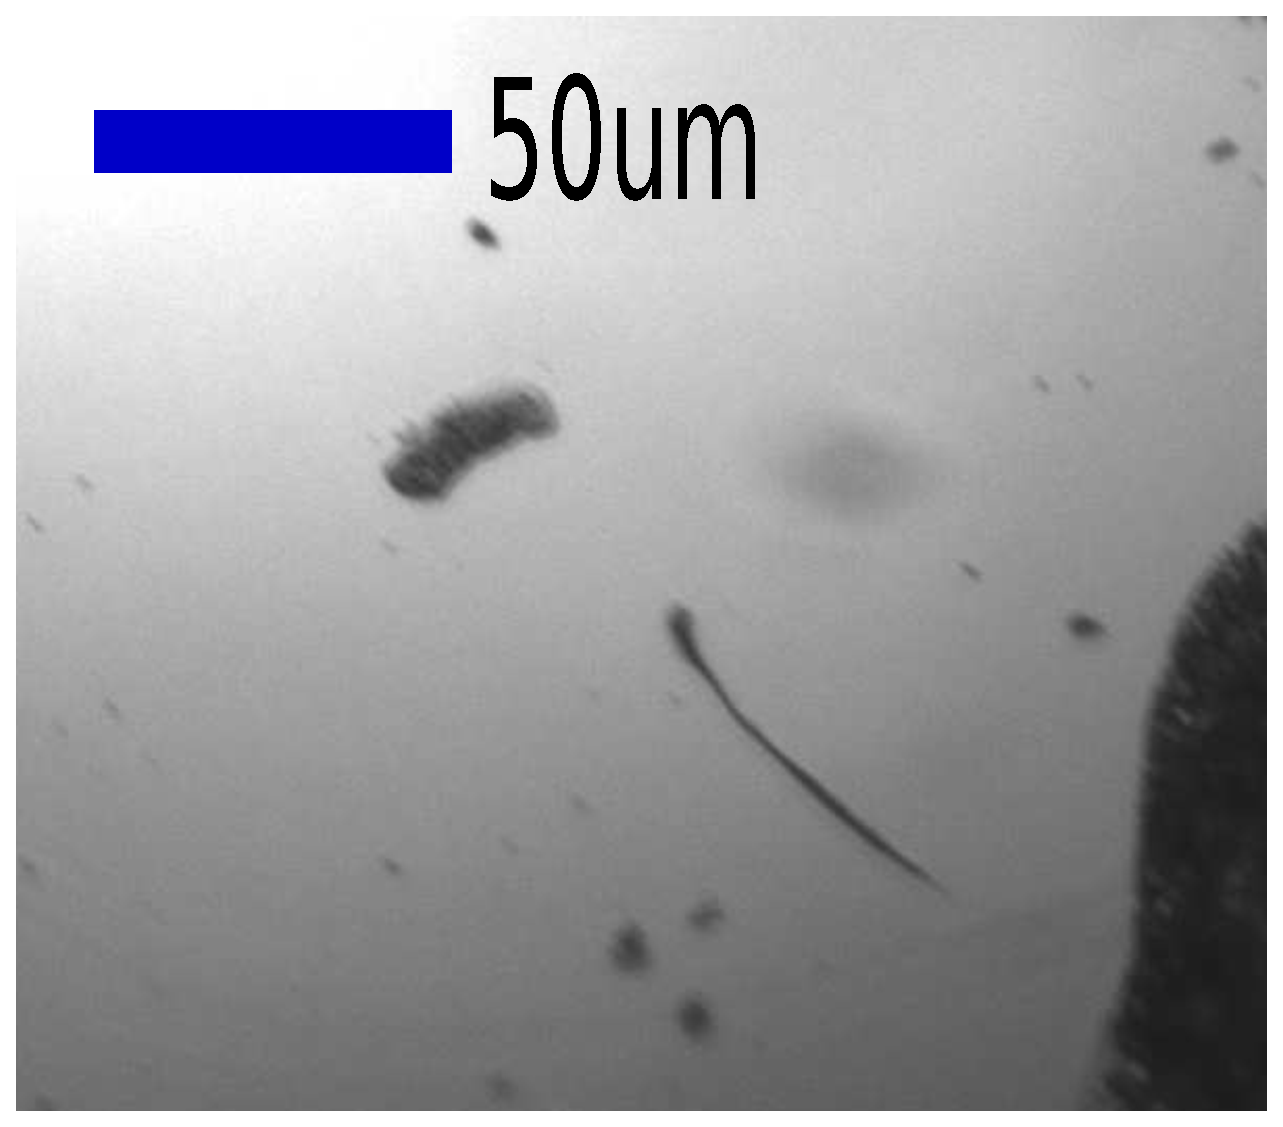
\includegraphics[width=\hsize]{nonpol300.eps}
  \end{center}
  \caption{無偏光@300K}
  \label{fig:nonpol300}
 \end{minipage}
 \begin{minipage}{0.333\hsize}
  \begin{center}
   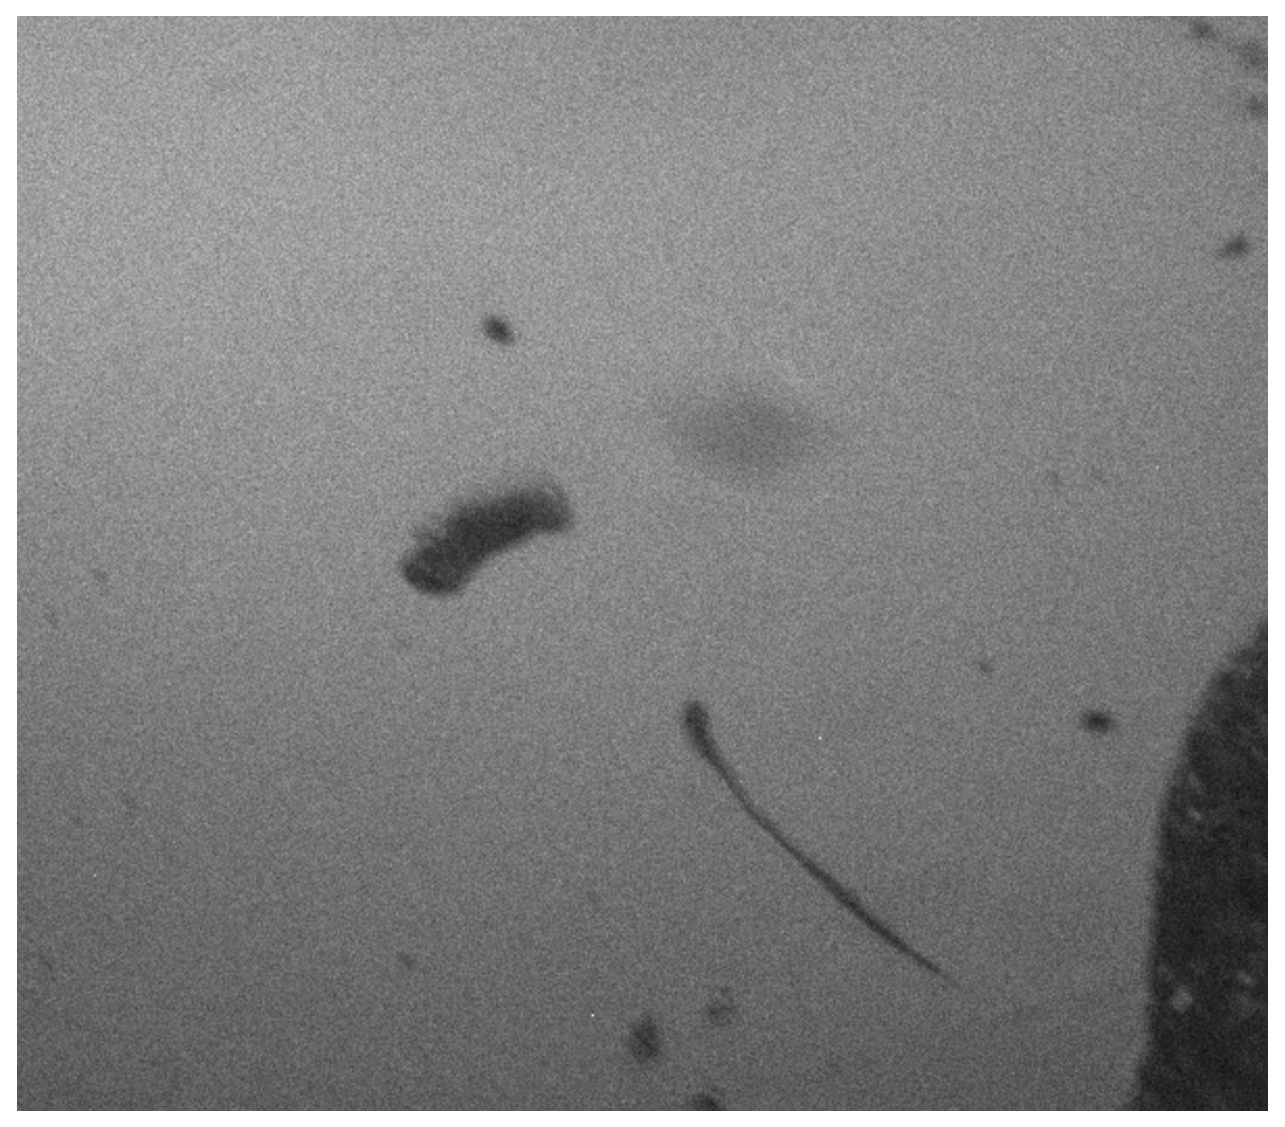
\includegraphics[width=\hsize]{hh300.eps}
  \end{center}
  \caption{平行偏光(x偏光/x検出)@300K}
  \label{fig:hh300}
 \end{minipage}
 \begin{minipage}{0.333\hsize}
  \begin{center}
   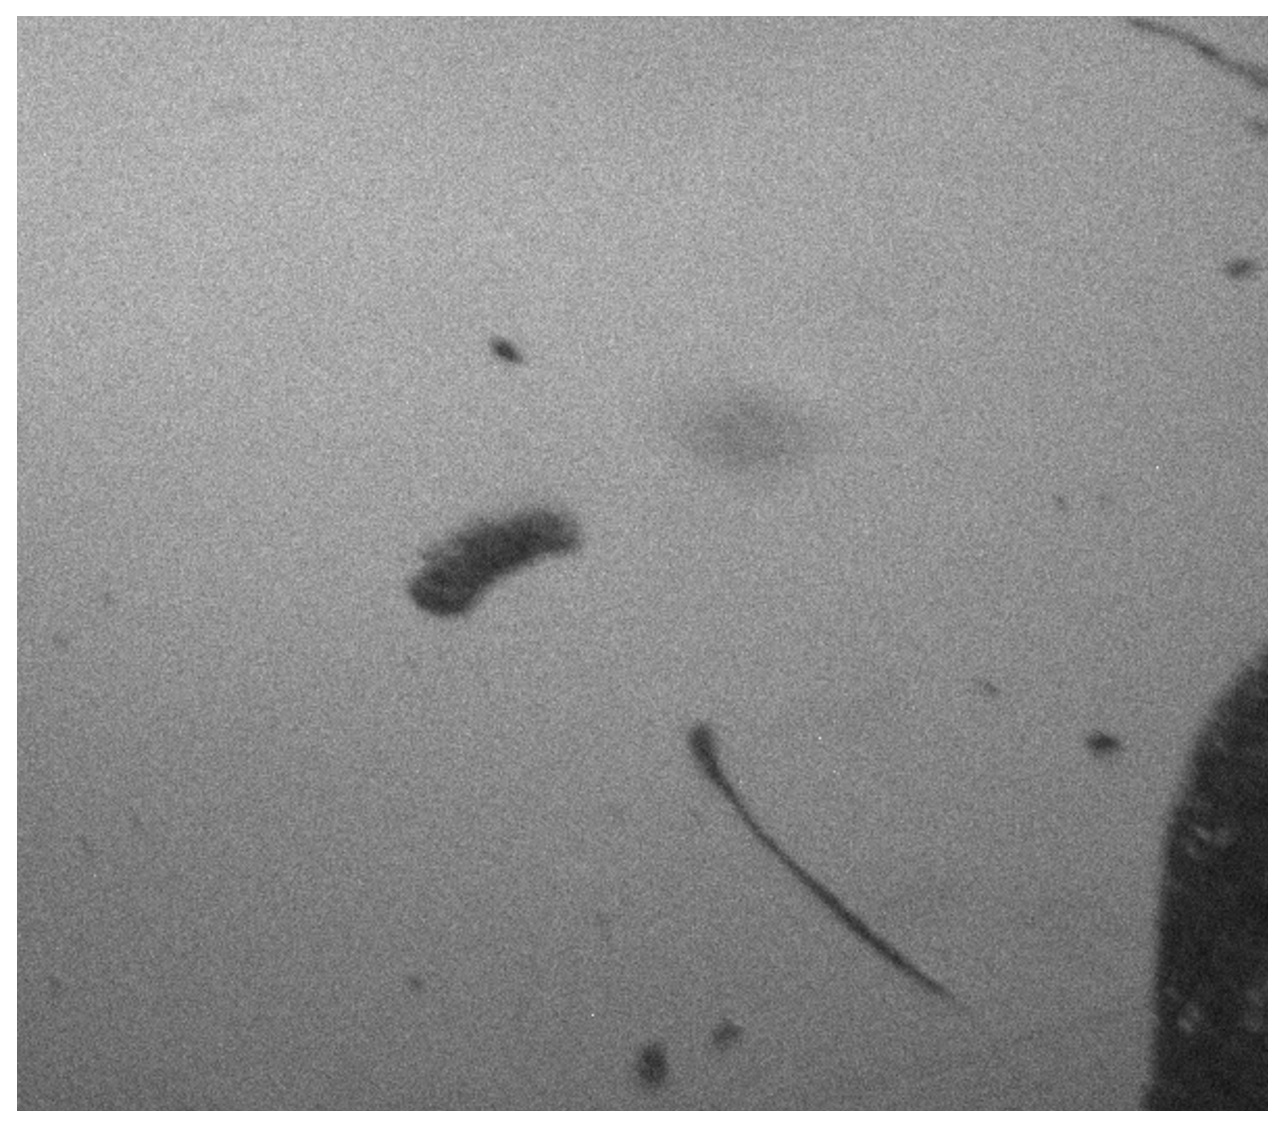
\includegraphics[width=\hsize]{vv300.eps}
  \end{center}
  \caption{平行偏光(y偏光/y検出)@300K}
  \label{fig:vv300}
 \end{minipage}
 \begin{minipage}{0.333\hsize}
  \begin{center}
   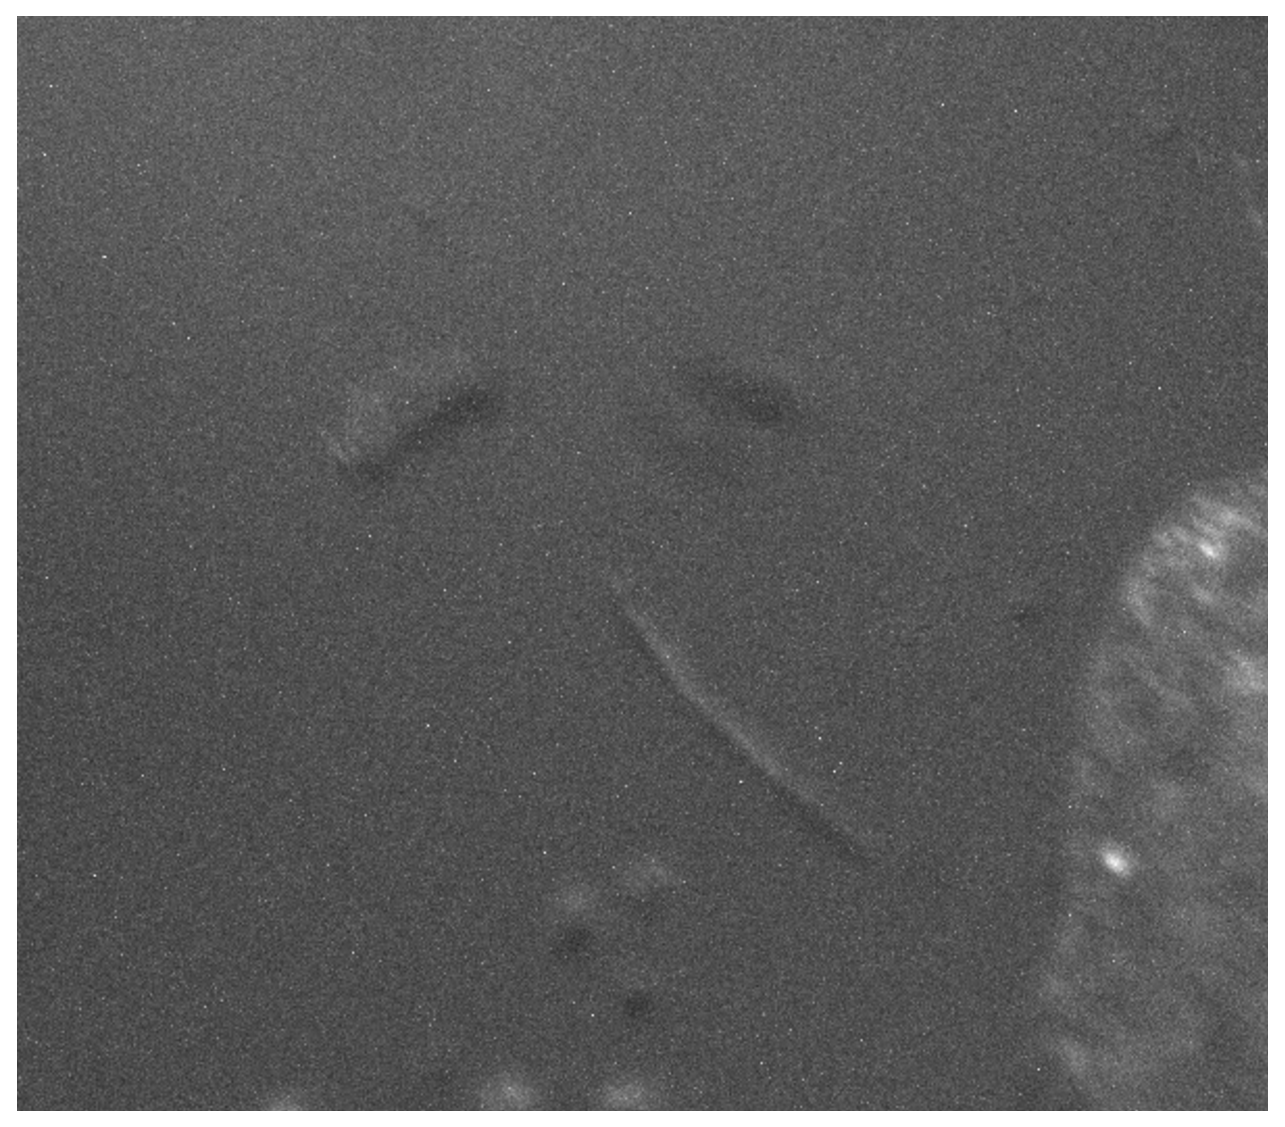
\includegraphics[width=\hsize]{vh300.eps}
  \end{center}
  \caption{直交偏光(y偏光/x検出)@300K}
  \label{fig:vh300}
 \end{minipage}
 \begin{minipage}{0.333\hsize}
  \begin{center}
   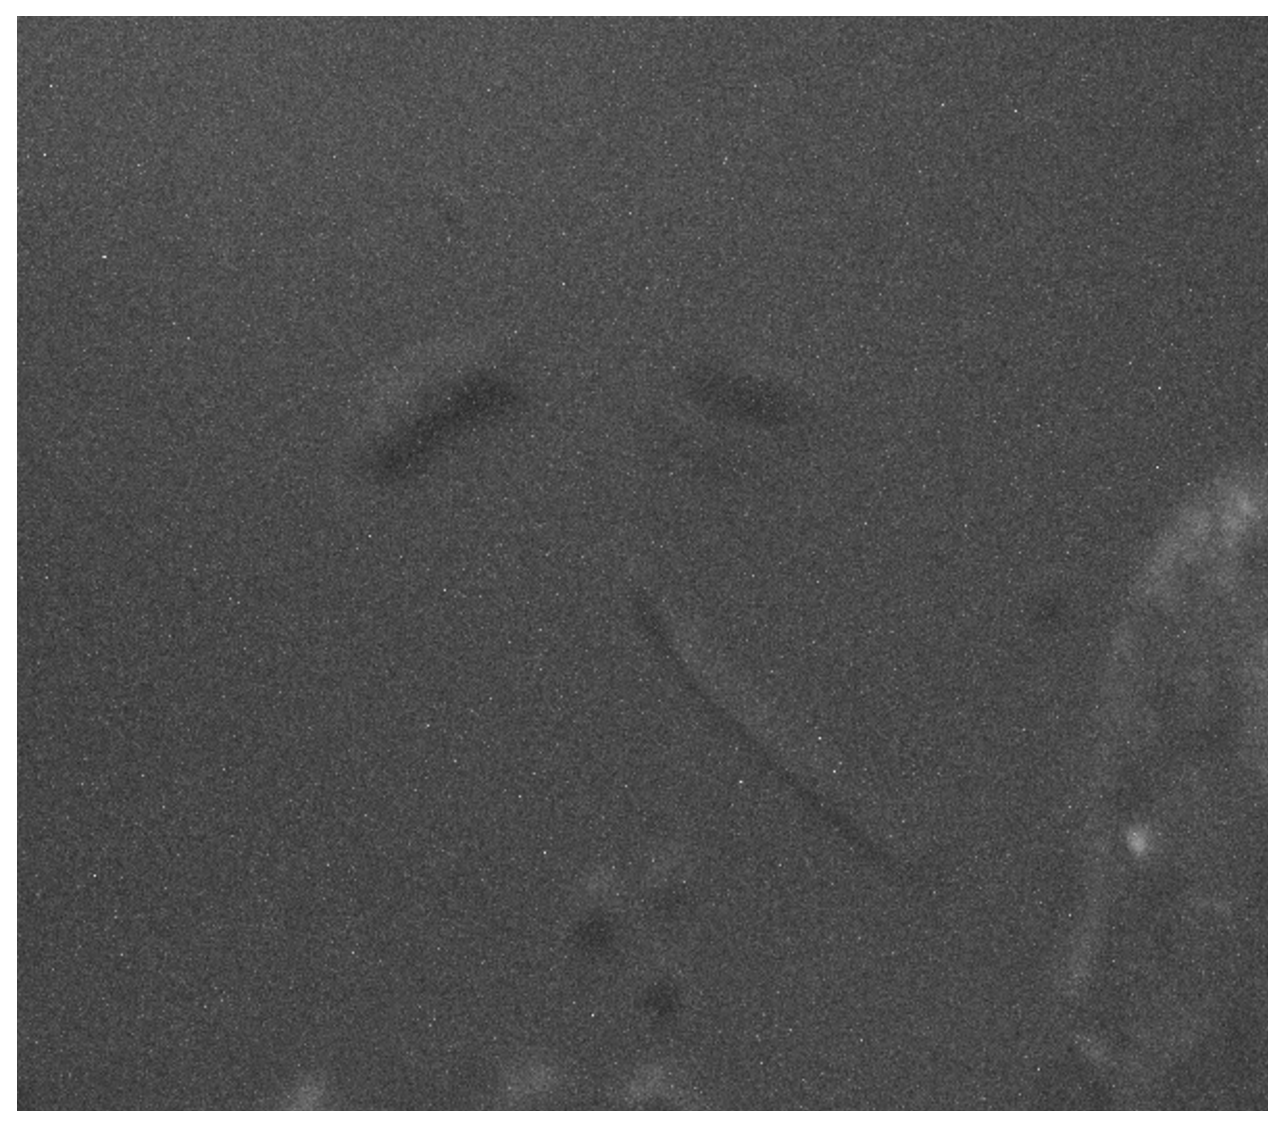
\includegraphics[width=\hsize]{hv300.eps}
  \end{center}
  \caption{直交偏光(x偏光/y検出)@300K}
  \label{fig:hv300}
 \end{minipage}
 \begin{minipage}{0.333\hsize}
  \begin{center}
   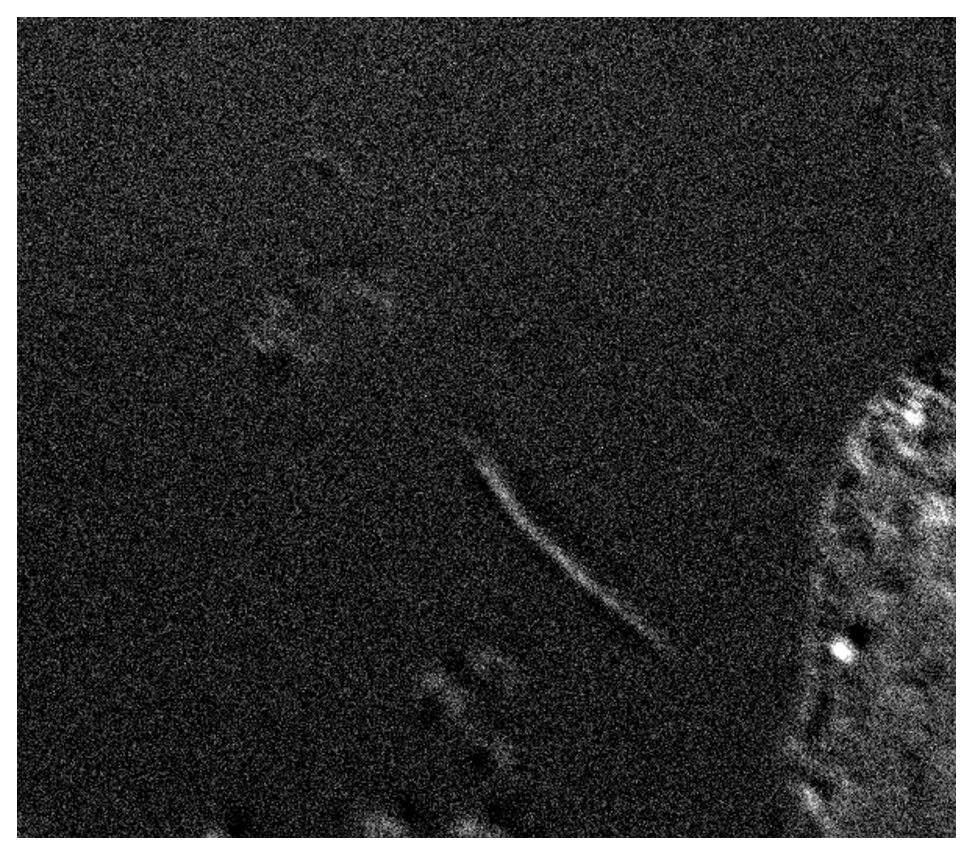
\includegraphics[width=\hsize]{vh300_subtractedby_hv300.eps}
  \end{center}
  \caption{図\ref{fig:vh300}と図\ref{fig:hv300}の差分@300K}
  \label{fig:vh300_subtractedby_hv300}
 \end{minipage}
 \begin{minipage}{0.333\hsize}
  \begin{center}
   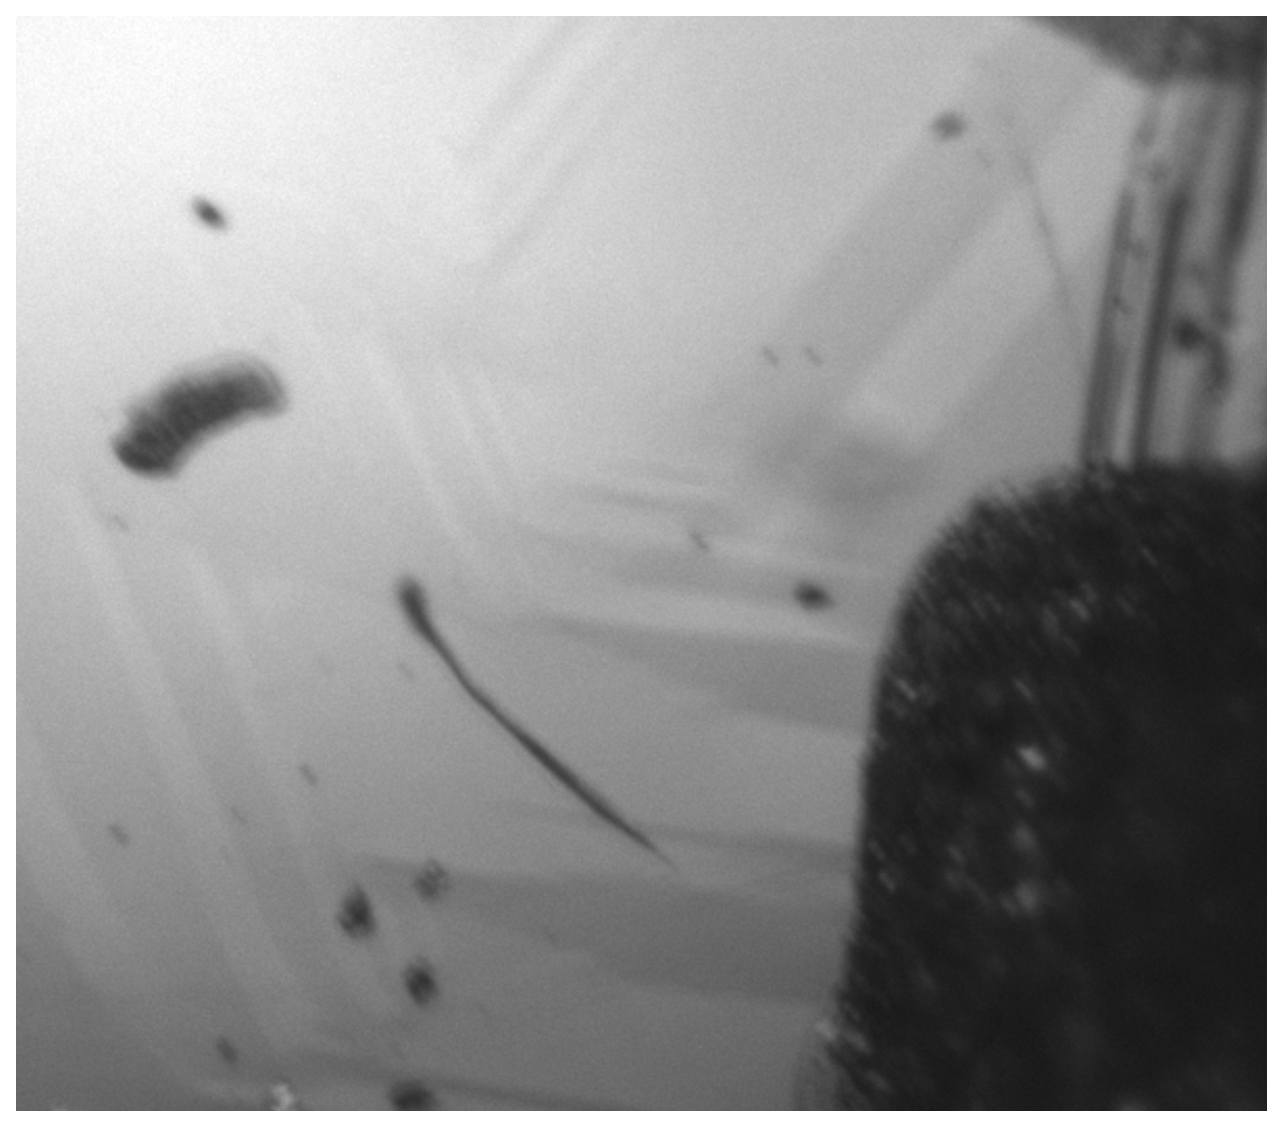
\includegraphics[width=\hsize]{nonpol250.eps}
  \end{center}
  \caption{無偏光@250K}
  \label{fig:nonpol250}
 \end{minipage}
 \begin{minipage}{0.333\hsize}
  \begin{center}
   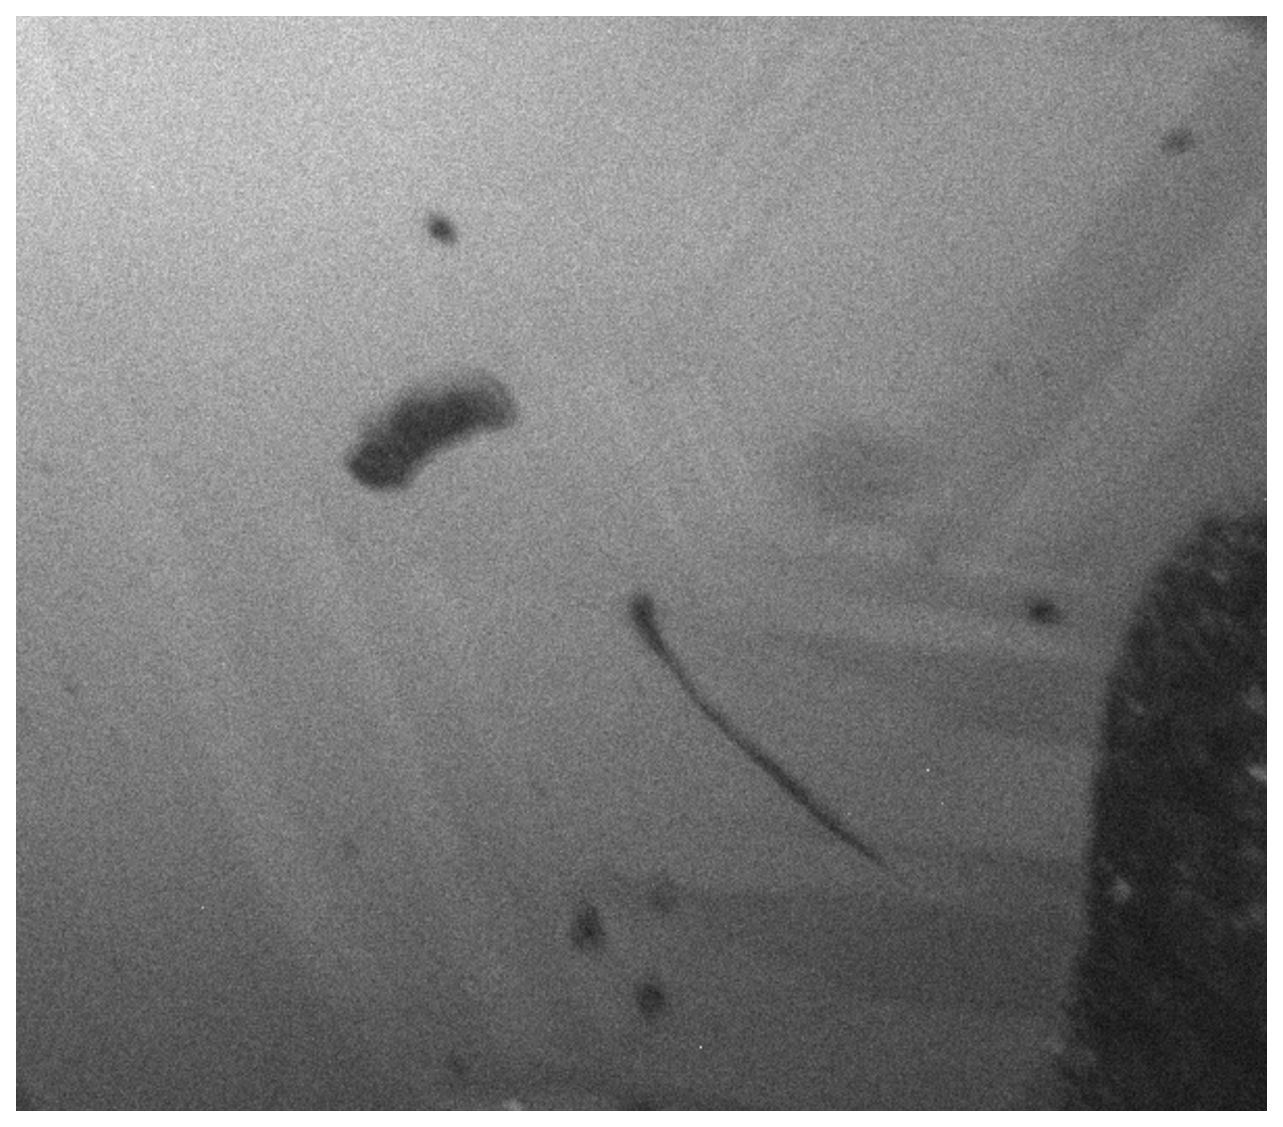
\includegraphics[width=\hsize]{hh250.eps}
  \end{center}
  \caption{平行偏光(x偏光/x検出)@250K}
  \label{fig:hh250}
 \end{minipage}
 \begin{minipage}{0.333\hsize}
  \begin{center}
   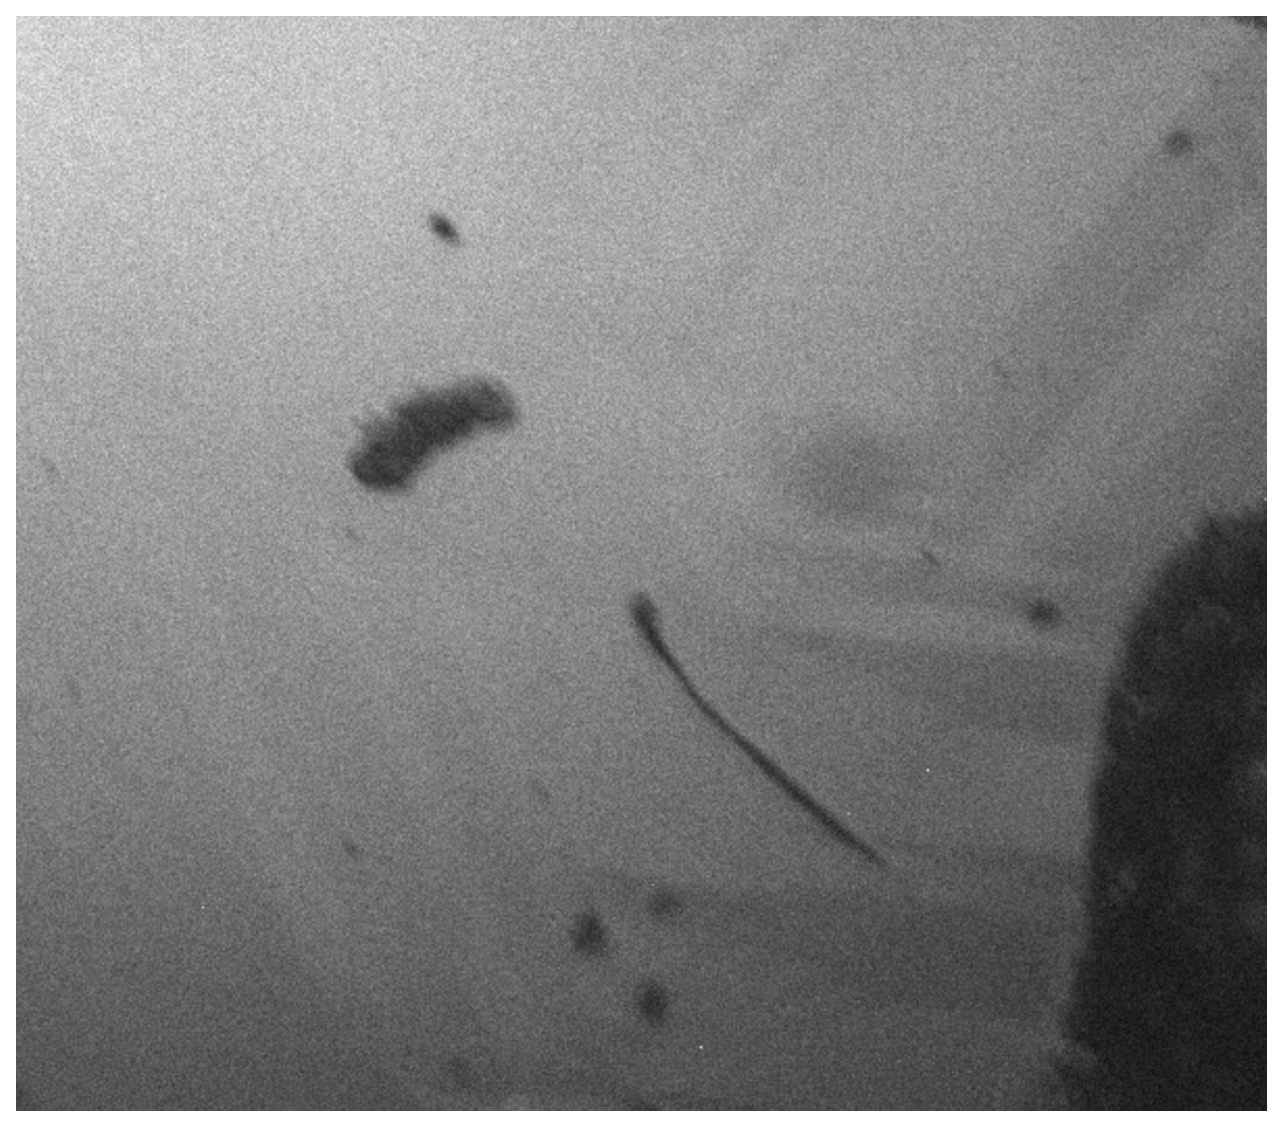
\includegraphics[width=\hsize]{vv250.eps}
  \end{center}
  \caption{平行偏光(y偏光/y検出)@250K}
  \label{fig:vv250}
 \end{minipage}
 \begin{minipage}{0.333\hsize}
  \begin{center}
   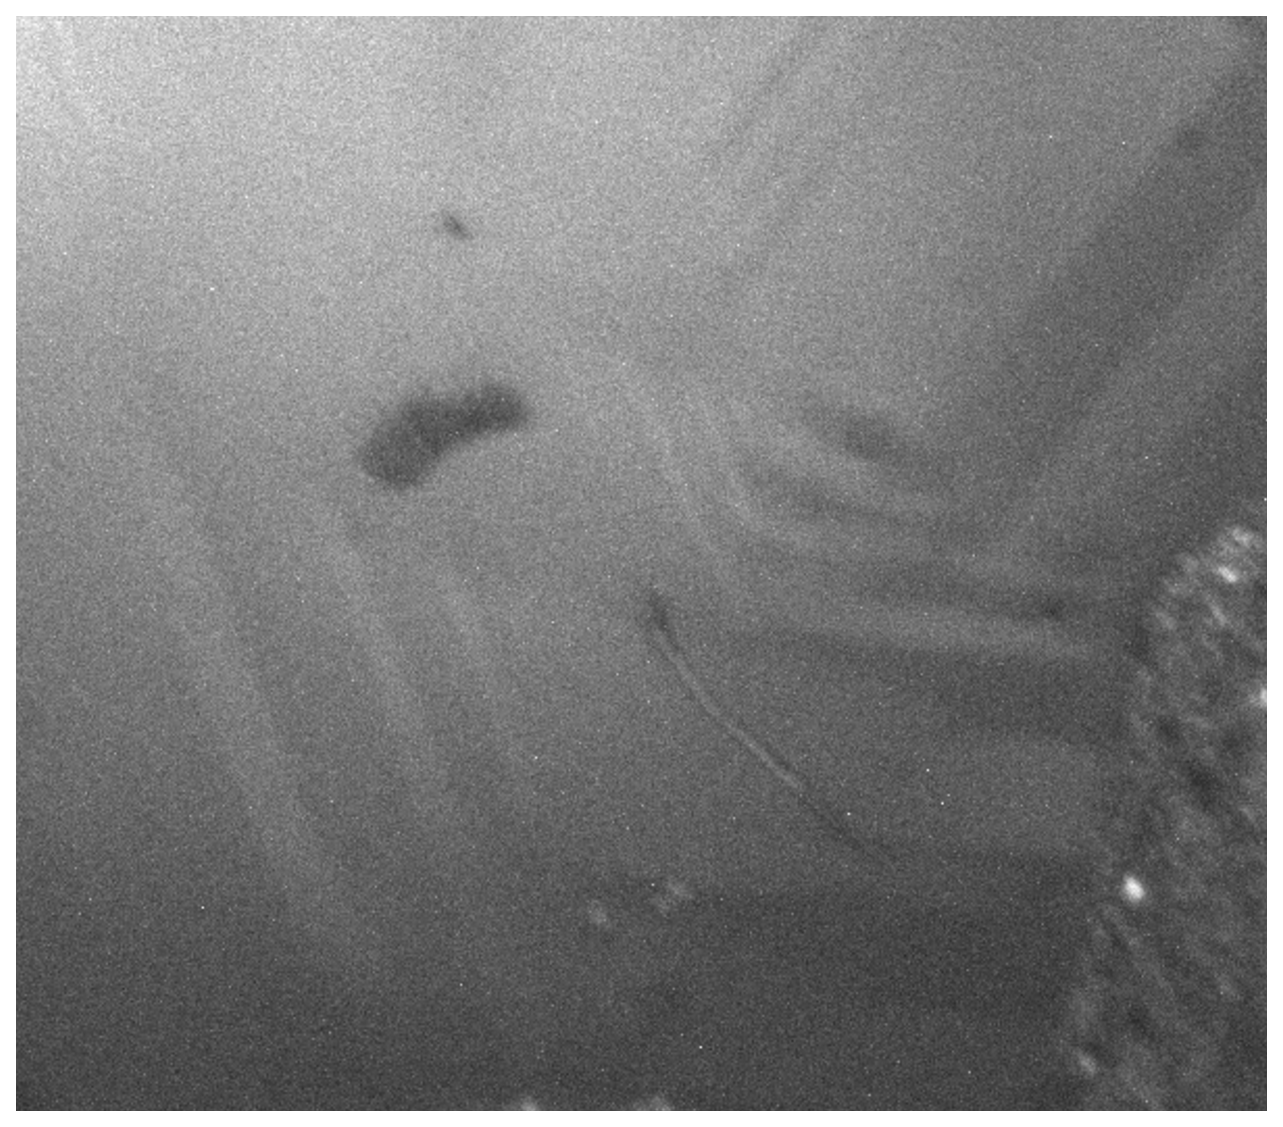
\includegraphics[width=\hsize]{vh250.eps}
  \end{center}
  \caption{直交偏光(y偏光/x検出)@250K}
  \label{fig:vh250}
 \end{minipage}
 \begin{minipage}{0.333\hsize}
  \begin{center}
   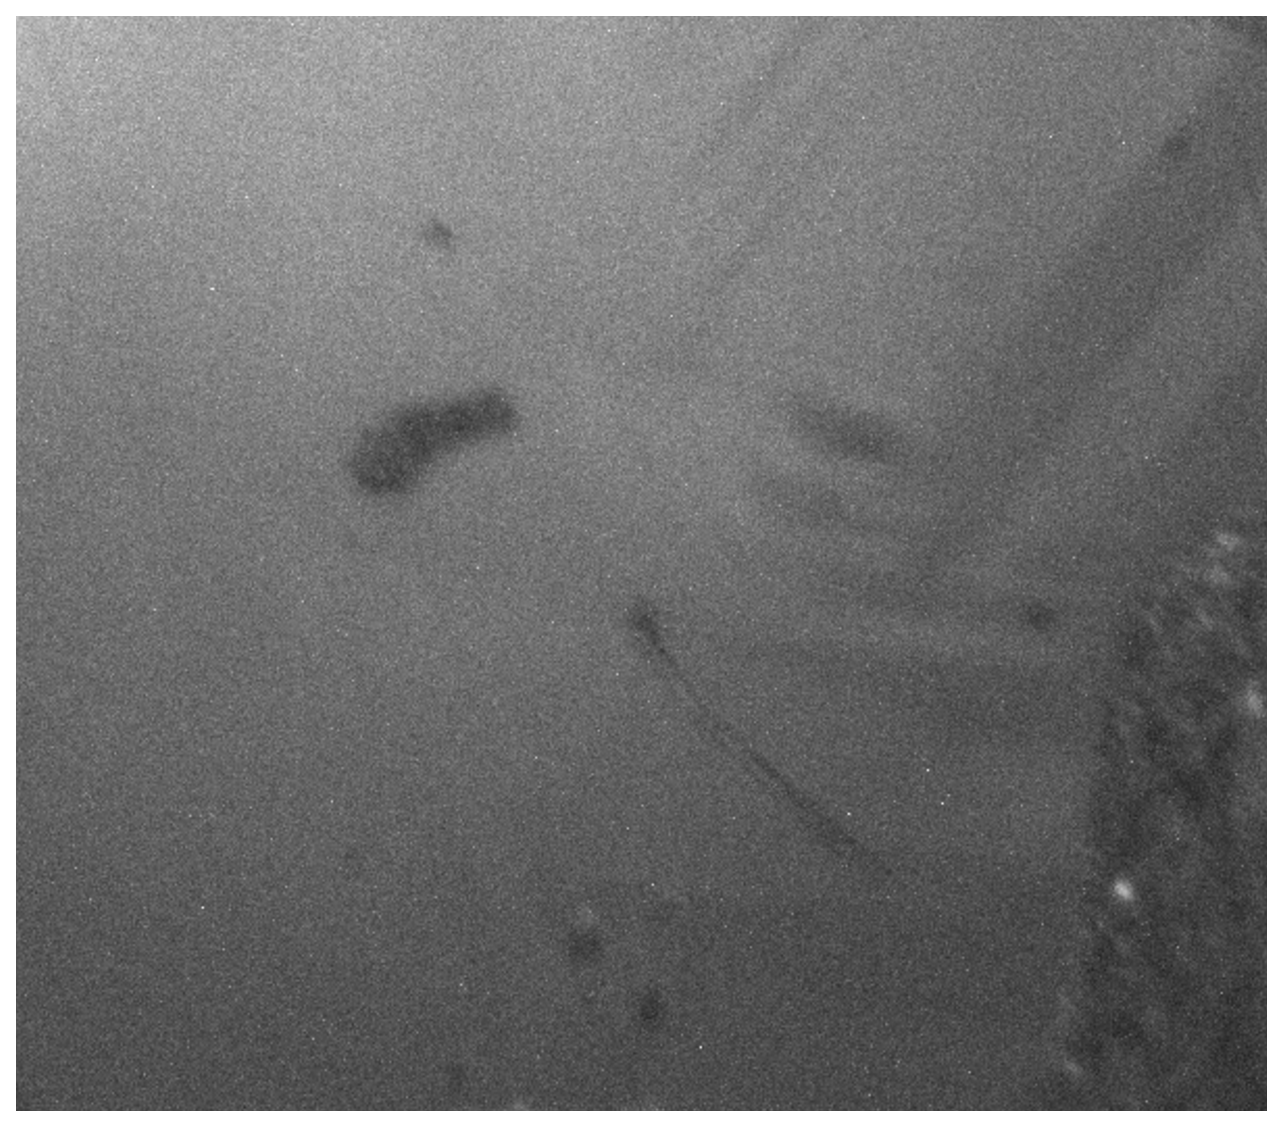
\includegraphics[width=\hsize]{hv250.eps}
  \end{center}
  \caption{直交偏光(x偏光/y検出)@250K}
  \label{fig:hv250}
 \end{minipage}
 \begin{minipage}{0.333\hsize}
  \begin{center}
   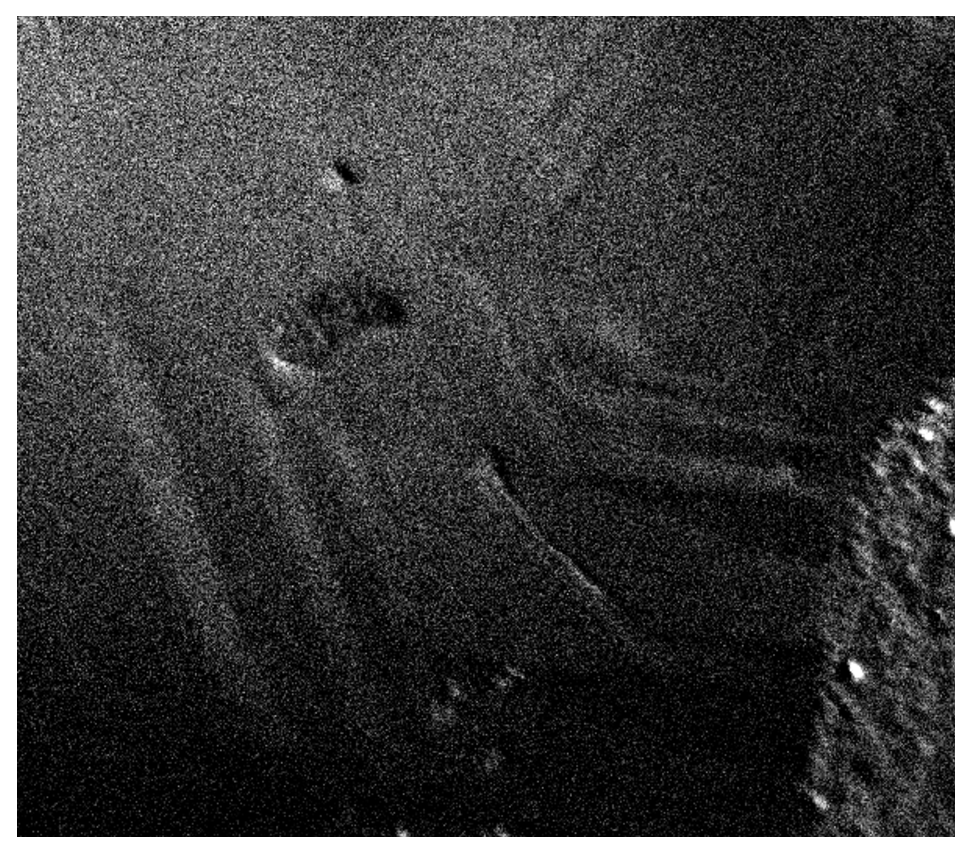
\includegraphics[width=\hsize]{vh250_subtractedby_hv250.eps}
  \end{center}
  \caption{図\ref{fig:vh250}と図\ref{fig:hv250}の差分@250K}
  \label{fig:vh250_subtractedby_hv250}
 \end{minipage}
\end{figure}

\begin{figure}[p]
  \begin{center}
   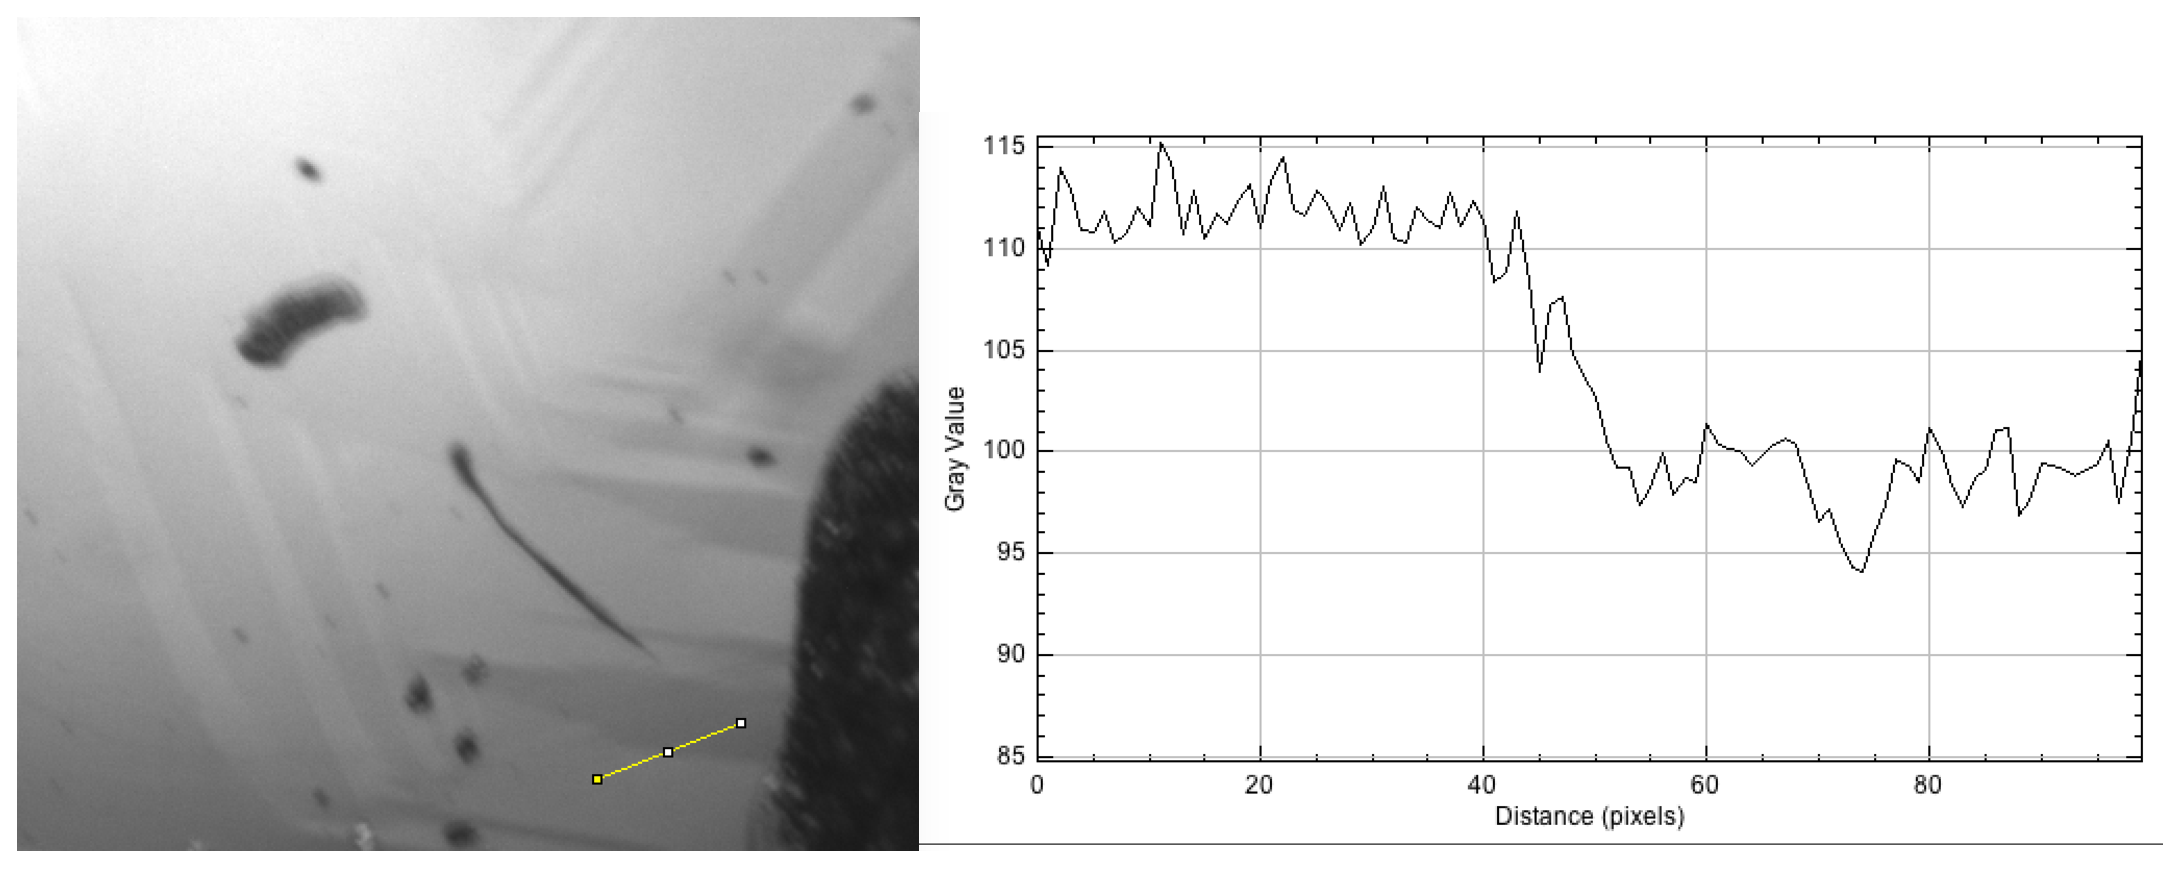
\includegraphics[width=0.8\hsize]{nonpol250_profile.eps}
  \end{center}
  \caption{信号強度のプロファイル(無偏光)@250K}
  \label{fig:nonpol250_profile}
\end{figure}

\subsection{250Kと50Kの偏光顕微鏡像の比較}
低温相の比較をするために、試料の温度を室温300Kから50Kまでレート1K/minで冷却したあと、同一のレートで50Kから300Kまで加熱した。冷却・加熱レート1K/minは前節で250Kから300Kまで温度掃引したときと同一である。図\ref{fig:resistance50-300}に温度と抵抗のヒステリシス曲線を示す。冷却中は270K付近と110K付近で少なくとも2回、不連続に抵抗が変化した。加熱中は240K付近のなだらかで特徴的な抵抗変化と、280K付近の不連続な抵抗変化が見られる。

図\ref{fig:microscope}の偏光顕微光学系から偏光子を取り去り、検光子をy方向に調整した光学系で、試料の冷却中に250Kと100K、50Kで偏光顕微鏡写真をとった。図\ref{fig:nonpolv250}と図\ref{fig:nonpolv100}、図\ref{fig:nonpolv50}にそれぞれ示す。さらに図\ref{fig:microscope}の偏光顕微光学系から偏光子と検光子をともに取り去った光学系で、試料の加熱中に50Kと150K、250K、300Kで無偏光の顕微鏡写真をとった。図\ref{fig:nonpol50_2}と図\ref{fig:nonpol150_2}、図\ref{fig:nonpol250_2}、図\ref{fig:nonpol300_2}にそれぞれ示す。一連の顕微鏡像は、前節の顕微鏡像と同一の領域を同じ倍率で撮影したものである。光源の明るさとCCDの動作条件は、図\ref{fig:nonpolv250}と図\ref{fig:nonpolv100}と図\ref{fig:nonpolv50}で同一であり、また図\ref{fig:nonpol50_2}と図\ref{fig:nonpol150_2}と図\ref{fig:nonpol250_2}と図\ref{fig:nonpol300_2}で同一である。ただし前節の顕微鏡像に比べて、光源の明るさとCCDの動作条件、光学系のセットアップが異なる。

検光子のみの条件で撮影した図\ref{fig:nonpolv250}は前節の250Kで撮影した無偏光の条件(図\ref{fig:nonpol250})と平行偏光の条件(図\ref{fig:vv250})と光学実験の条件が異なるが、冷却のレート1K/minは同一である。これらの図を比較してみると、明らかに異なる明暗のパターンが現れていることが分かる。したがって300Kから250Kまで同一のレート1K/minで繰り返し冷却しても、顕微鏡写真に現れる明暗のパターンは再現しないことが分かる。

250Kで撮影した図\ref{fig:nonpolv250}と100Kで撮影した図\ref{fig:nonpolv100}を比較すると、冷却により明暗のパターンが変化し、コントラストが小さくなったことが分かる。

冷却中に図\ref{fig:nonpolv100}(100K)で観察された顕微鏡写真に特徴的なパターンは、検光子のみの光学系で撮影された図\ref{fig:nonpolv50}(50K)と無偏光の光学系で撮影された図\ref{fig:nonpol50_2}(50K)でともに観察される。新しく現れた低温相に特徴的なパターンは、図\ref{fig:nonpol250_2}から分かるように加熱していったとき遅くとも250Kまで保たれた。

最後に本節で得られた結果をまとめる。
\begin{enumerate}
\item 300Kから250Kまで同一のレート1K/minで繰り返し冷却しても、顕微鏡写真に現れる明暗のパターンは再現しない
\item 250Kから100Kまでレート1K/minで冷却してゆき、冷却前後で顕微鏡写真を比較すると、明暗のパターンが変化し、コントラストが小さくなった(図\ref{fig:nonpolv250}、図\ref{fig:nonpolv100})
\item 50Kの低温相の顕微鏡写真に特徴的な明暗のパターンは、加熱してゆくと250Kでも保たれた(図\ref{fig:nonpol50_2}、図\ref{fig:nonpol150_2}、図\ref{fig:nonpol250_2})
 \end{enumerate}

\begin{figure}[p]
  \begin{center}
   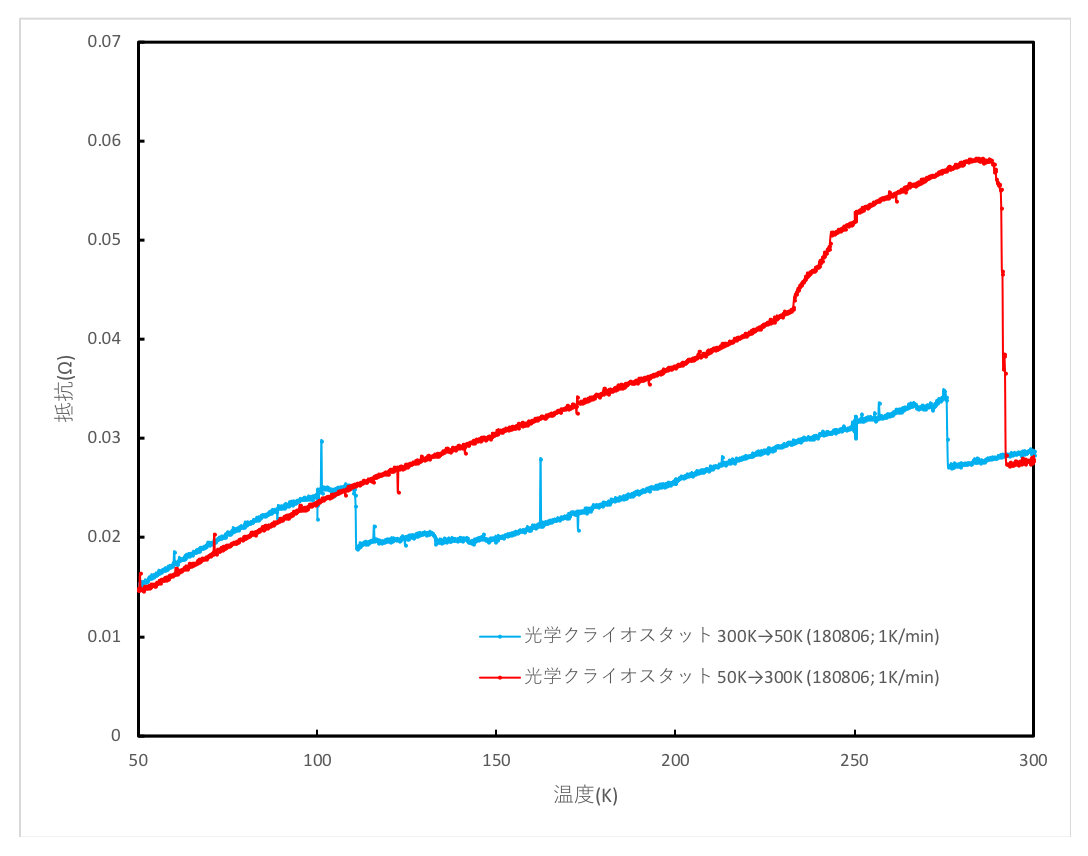
\includegraphics[width=150mm]{resistance50-300.eps}
  \end{center}
  \caption{抵抗の温度依存性}
  \label{fig:resistance50-300}
\end{figure}

\begin{figure}[p]
 \begin{minipage}{0.333\hsize}
  \begin{center}
   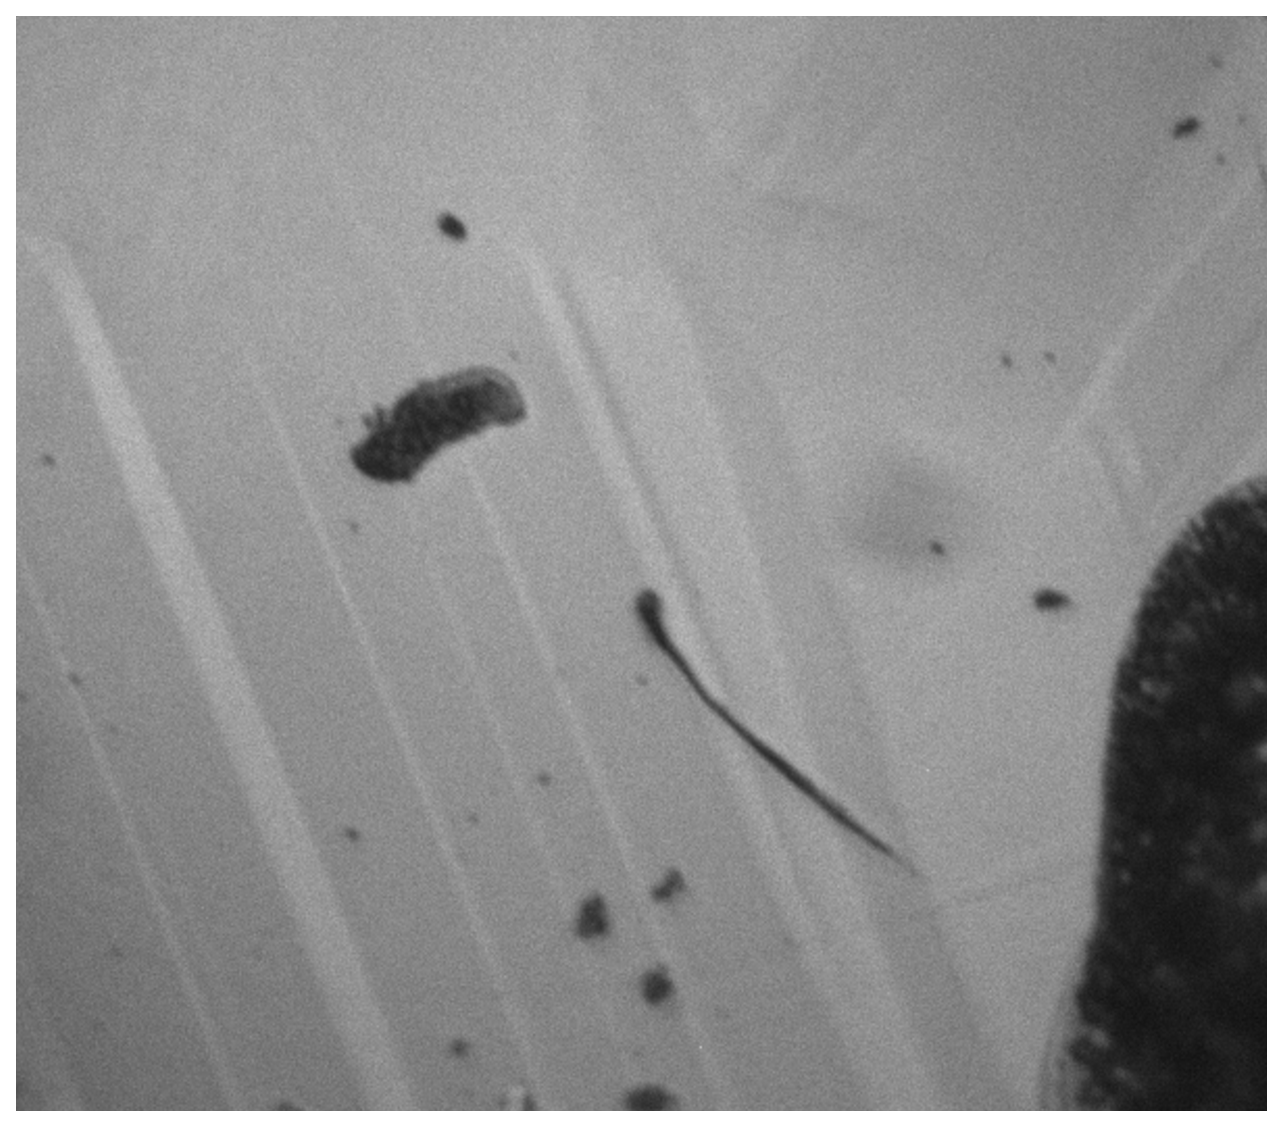
\includegraphics[width=\hsize]{nonpolv250.eps}
  \end{center}
  \caption{検光子のみ(y検出)@250K}
  \label{fig:nonpolv250}
 \end{minipage}
 \begin{minipage}{0.333\hsize}
  \begin{center}
   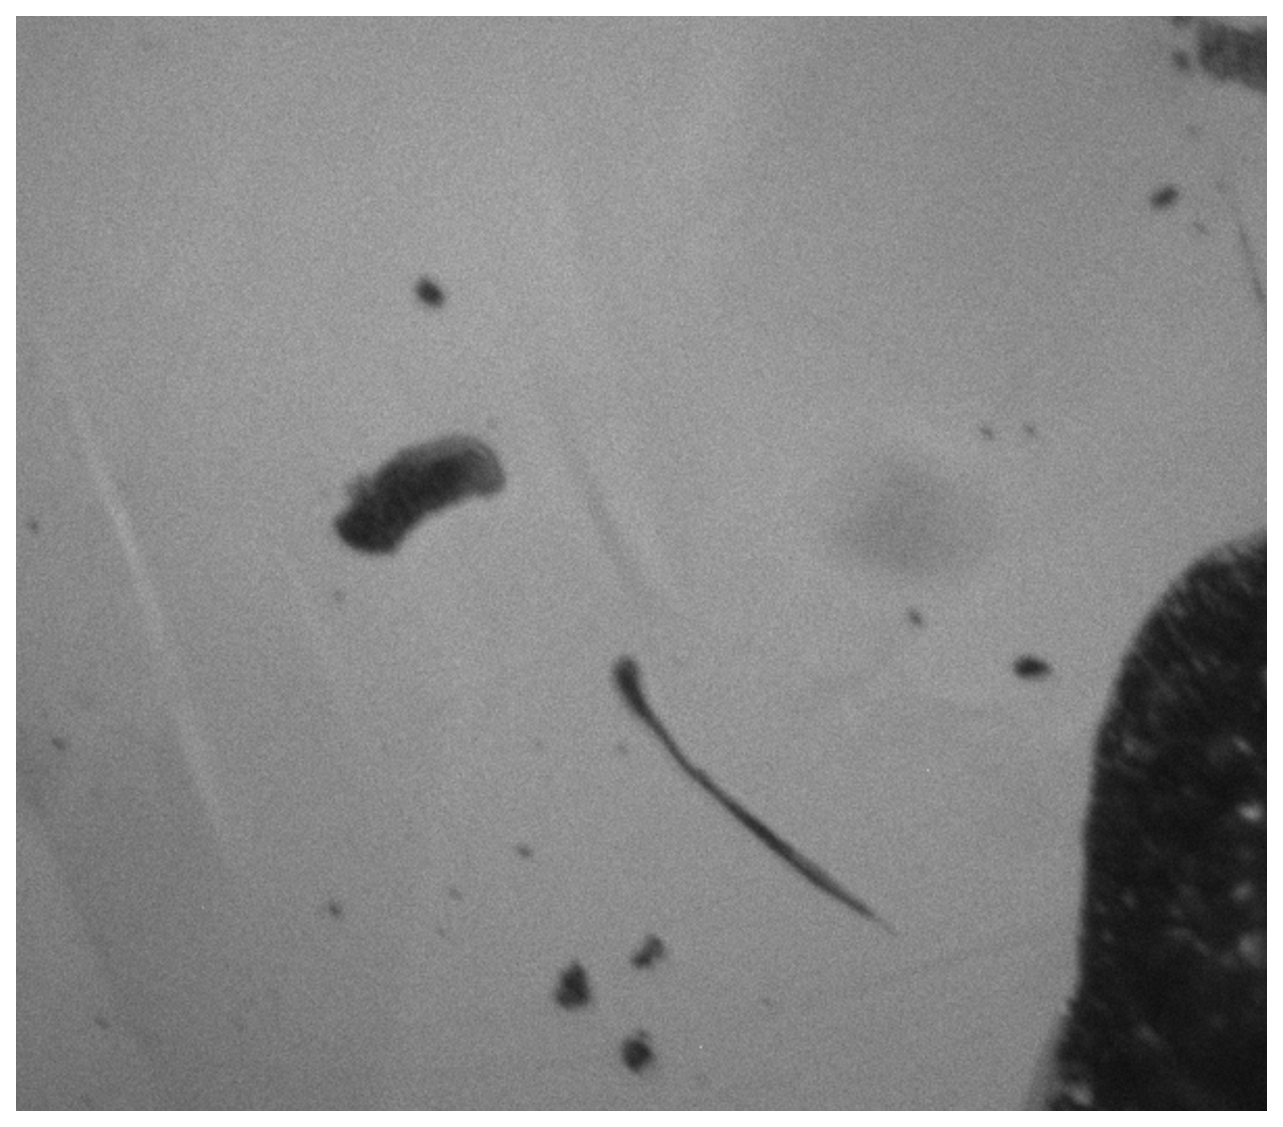
\includegraphics[width=\hsize]{nonpolv100.eps}
  \end{center}
  \caption{検光子のみ(y検出)@100K}
  \label{fig:nonpolv100}
 \end{minipage}
 \begin{minipage}{0.333\hsize}
  \begin{center}
   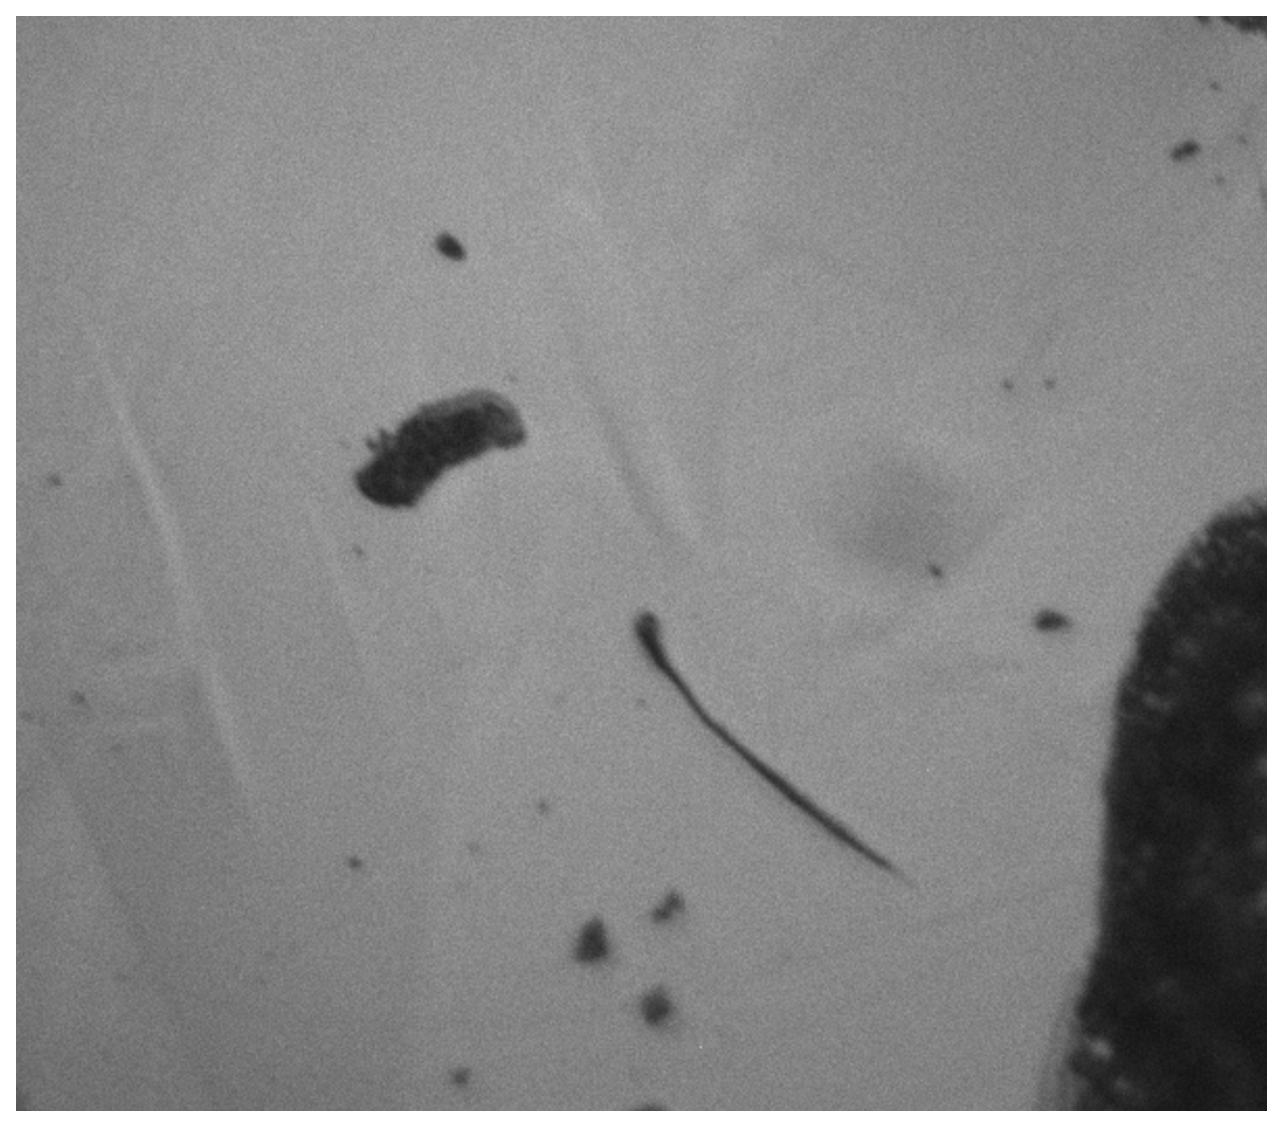
\includegraphics[width=\hsize]{nonpolv50.eps}
  \end{center}
  \caption{検光子のみ(y検出)@50K}
  \label{fig:nonpolv50}
 \end{minipage}
 \begin{minipage}{0.333\hsize}
  \begin{center}
   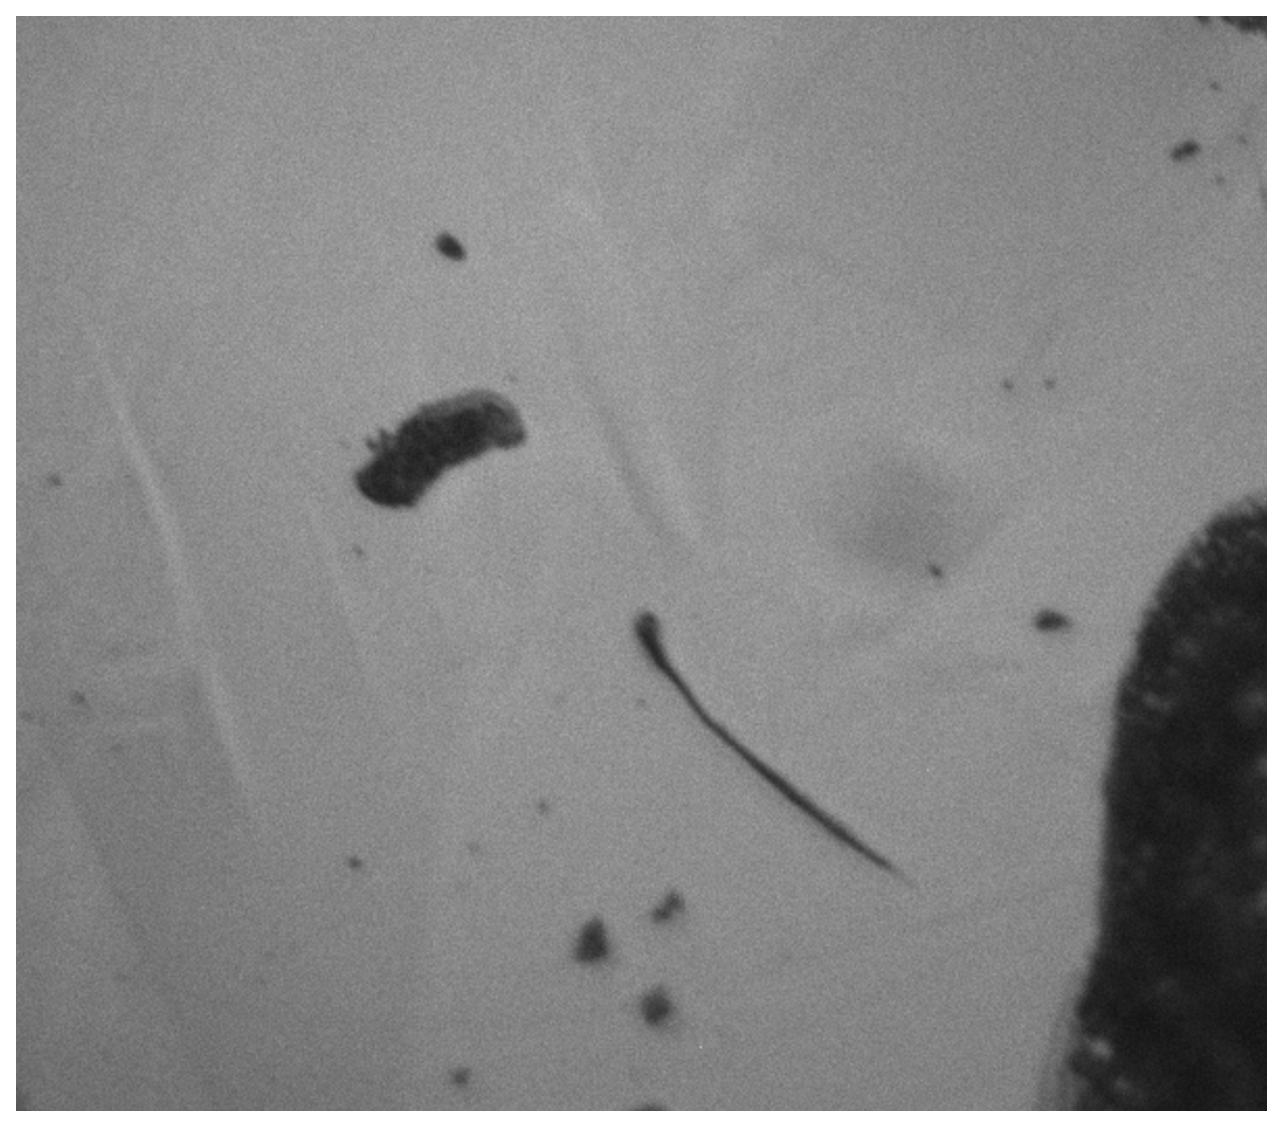
\includegraphics[width=\hsize]{nonpol50_2.eps}
  \end{center}
  \caption{無偏光@50K}
  \label{fig:nonpol50_2}
 \end{minipage}
  \begin{minipage}{0.333\hsize}
  \begin{center}
   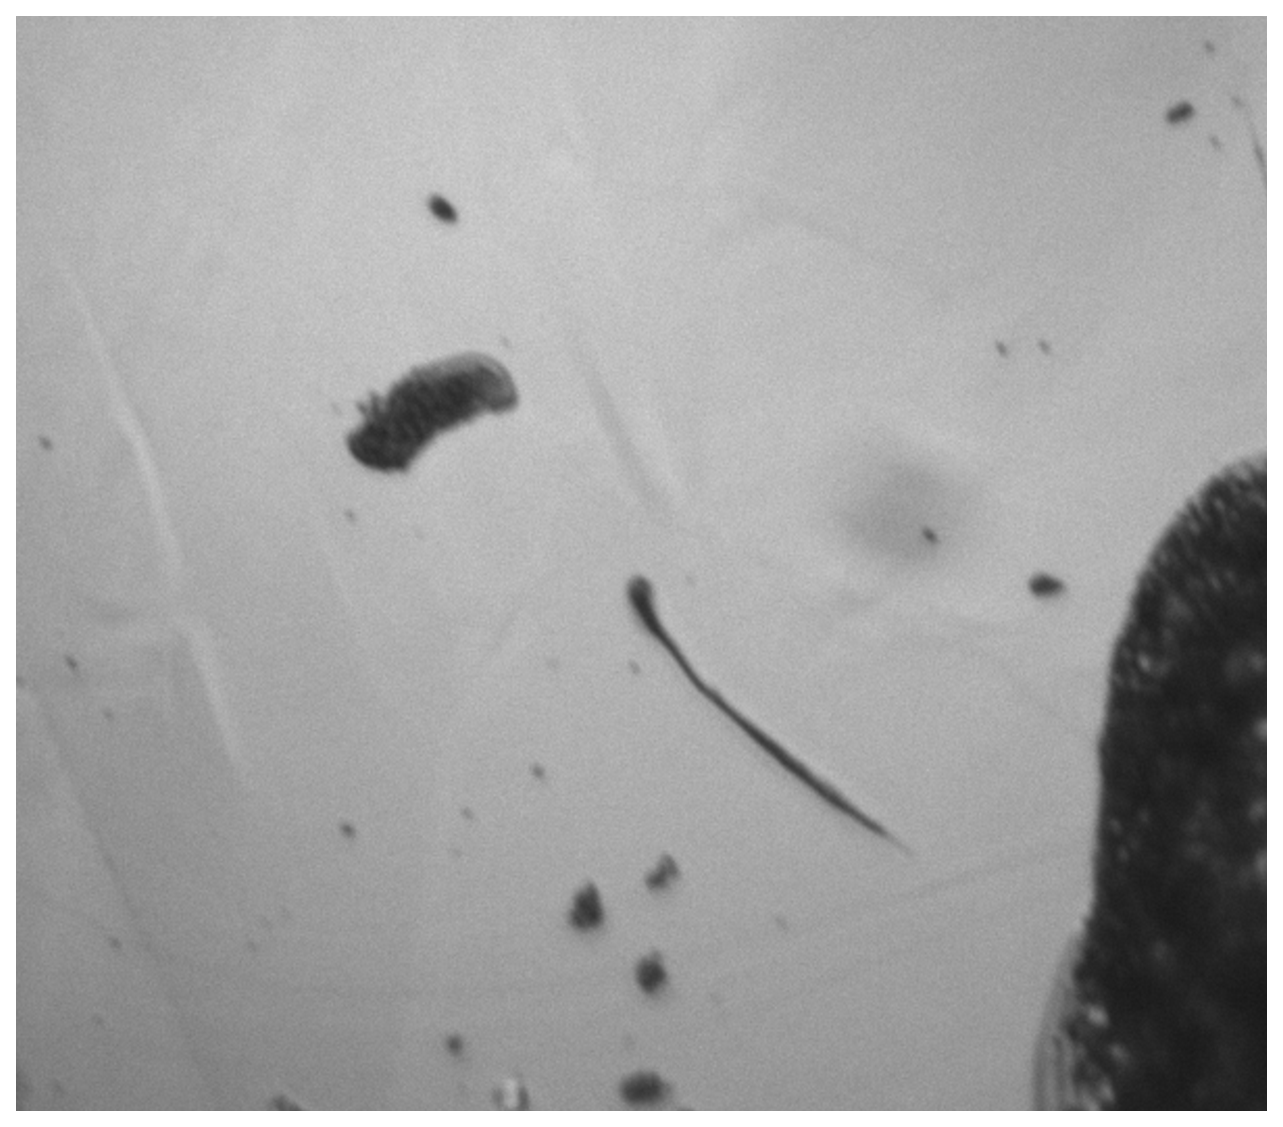
\includegraphics[width=\hsize]{nonpol150_2.eps}
  \end{center}
  \caption{無偏光@150K}
  \label{fig:nonpol150_2}
 \end{minipage}
 \begin{minipage}{0.333\hsize}
  \begin{center}
   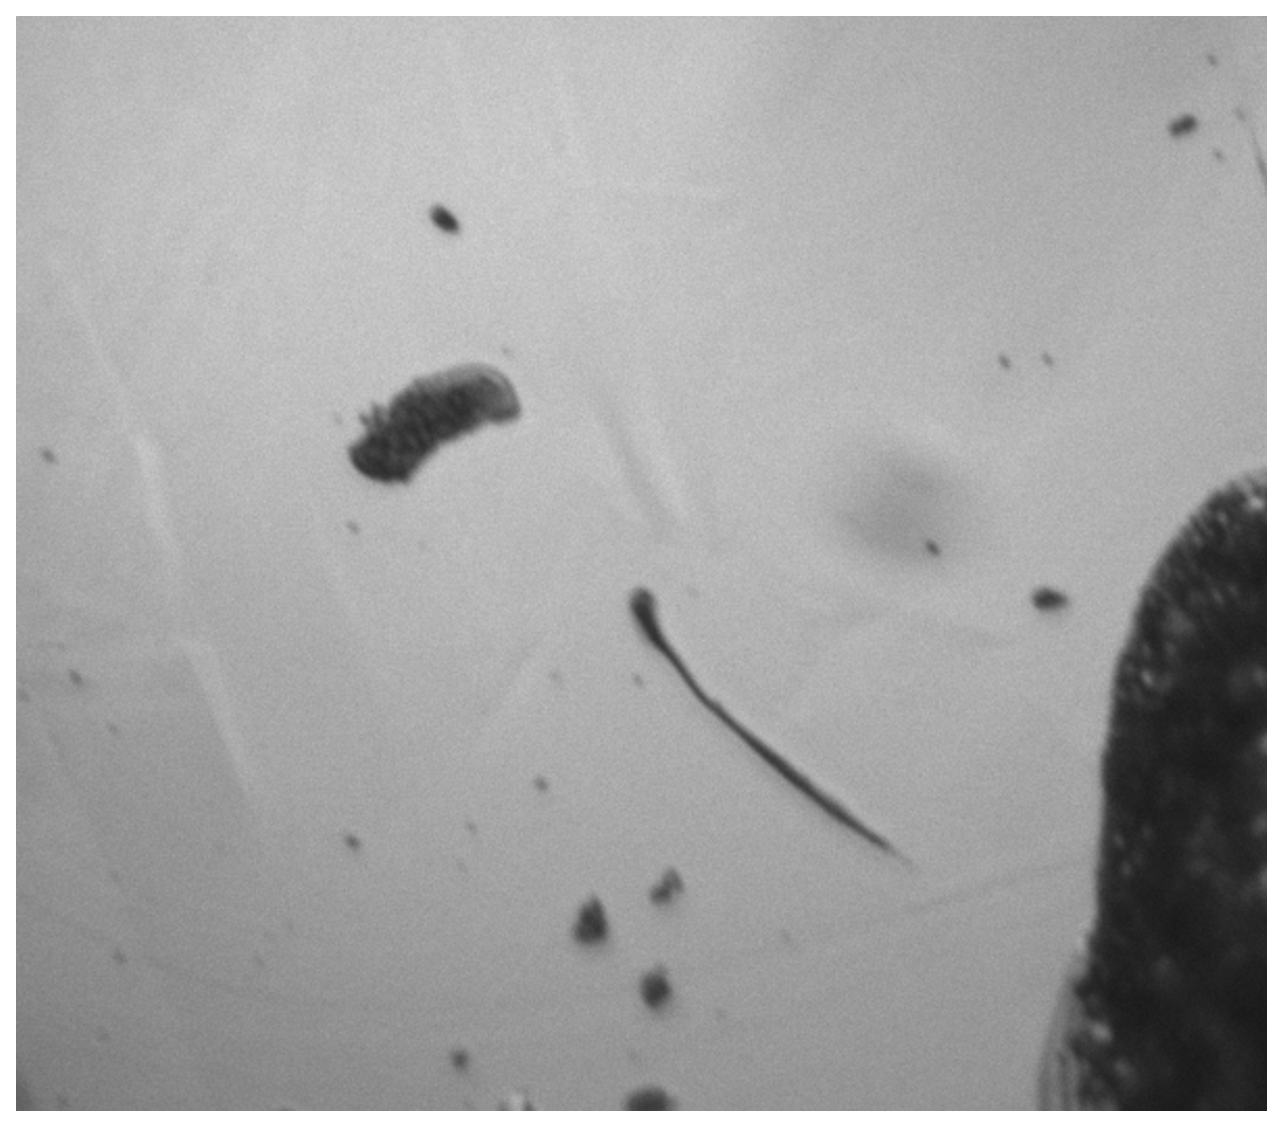
\includegraphics[width=\hsize]{nonpol250_2.eps}
  \end{center}
  \caption{無偏光@250K}
  \label{fig:nonpol250_2}
 \end{minipage}
 \begin{minipage}{0.333\hsize}
  \begin{center}
   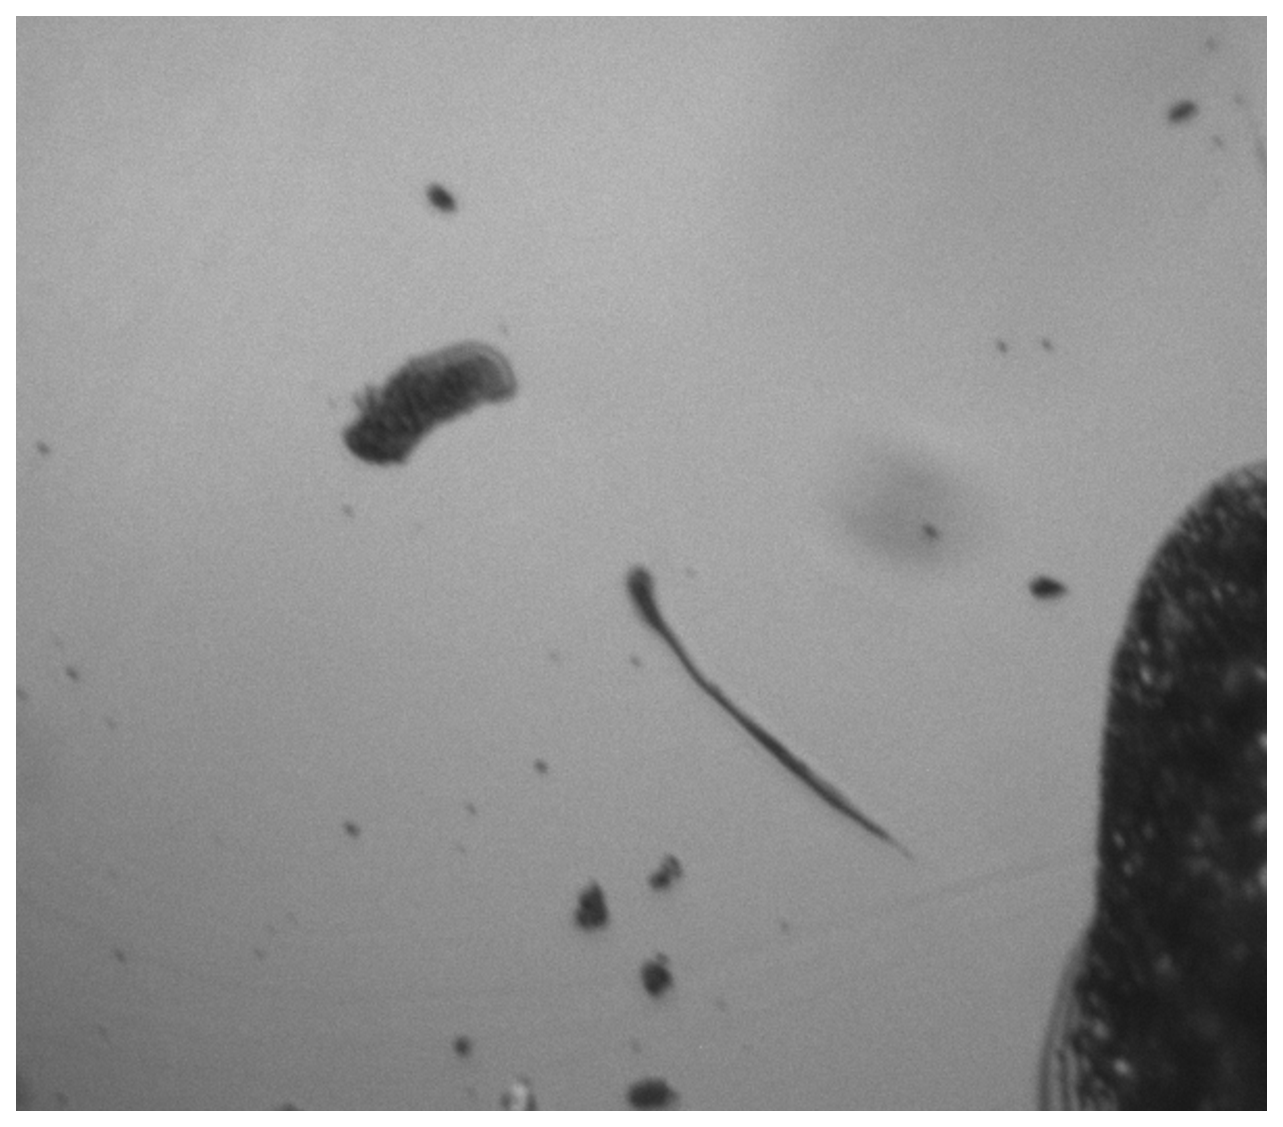
\includegraphics[width=\hsize]{nonpol300_2.eps}
  \end{center}
  \caption{無偏光@300K}
  \label{fig:nonpol300_2}
 \end{minipage}
\end{figure}



\section{議論}

\subsection{結果の考察}
偏光顕微鏡の観察から以下の結果が得られた。
\begin{description}
\item[300Kと250Kの偏光顕微鏡像の比較]
\item
\begin{enumerate}
\item 300Kから250Kまでレート1K/minで冷却してゆくと、300Kの顕微鏡写真に見られなかった明暗のパターンが、250Kの顕微鏡写真に現れた。その明暗のパターンは無偏光の条件(図\ref{fig:nonpol250})と平行偏光偏光条件(図\ref{fig:hh250}、\ref{fig:vv250})、直交偏光条件(図\ref{fig:vh250}、\ref{fig:hv250})の全条件に関して見て取れる。ただしコントラストは条件により異なる。
\item 明るい領域は、典型的に細長い形をしており、概ね$10 \mu m$オーダーの大きさを持つ。また明るい領域と暗い領域の境界の方向は三方向あり、お互いに概ね60度の角度をなしている。
\item 明るい領域と暗い領域の境界で信号強度は急峻に変化した。無偏光の条件で明るい領域と暗い領域のコントラストは13\%程度である(図\ref{fig:nonpol250_profile})
\item 直交偏光の条件で250Kの明るい領域は、周囲と比べて明るいだけでなく300Kの対応する領域に対しても明るい(図\ref{fig:vh300}、\ref{fig:vh250})
\item 直交偏光の条件で、明るく細長い領域が伸びる方向と偏光/検光方向に依存して周囲との明暗のコントラストが異なる(図\ref{fig:vh250} 、\ref{fig:hv250})
 \end{enumerate}
\item[250Kと50Kの偏光顕微鏡像の比較]
\item 
\begin{enumerate}
\item 300Kから250Kまで同一のレート1K/minで繰り返し冷却しても、顕微鏡写真に現れる明暗のパターンは再現しない
\item 250Kから100Kまでレート1K/minで冷却してゆき、冷却前後で顕微鏡写真を比較すると、明暗のパターンが変化し、コントラストが小さくなった(図\ref{fig:nonpolv250}、図\ref{fig:nonpolv100})
\item 50Kの低温相の顕微鏡写真に特徴的な明暗のパターンは、加熱してゆくと250Kでも保たれた(図\ref{fig:nonpol50_2}、図\ref{fig:nonpol150_2}、図\ref{fig:nonpol250_2})
 \end{enumerate}
 \end{description}
 
%%考察
得られた結果に関して以下のように筆者は考察する。
\begin{description}
\item[280K付近で現れた低温相に関して]
\item[]
試料を300Kから冷却してゆくと280K付近で、抵抗が不連続に変化し、顕微鏡像に明暗のパターンが現れた。また明暗のパターンの境界で、信号強度が急峻に変化した。これらの結果は少なくとも一部の領域に低温相が現れた証拠だと筆者は考える。この低温相に関して以下のことが言える:

\begin{description}
\item[低温相の異方性]
直交偏光の条件で250Kの明るい領域と300Kの対応する領域を比較すると、250Kの方が信号強度が強かった。これは低温相の明るい領域の異方的な反射率テンソルに起因する。また、直交偏光条件で偏光方向を変えると明るい領域と暗い領域のコントラストが変化した(図\ref{fig:vh250}、図\ref{fig:hv250})。この振る舞いは明るい領域と暗い領域の反射率がともに等方的であると仮定した場合、説明できない。したがって現れた低温相のうち少なくとも一部の領域で反射率テンソルは、異方的であることが確認できる。この異方的な反射率テンソルは、付録\ref{sec:IrTe2_reflectance_LT}で述べたように、低温相の結晶の対称性を反映したものである。
ただし、構築した光学系が理想的であると仮定すると、図\ref{fig:vh250}と図\ref{fig:hv250}の結果を説明できないことに注意する。付録\ref{sec:diagonazed_reflectance}より直交偏光条件で信号強度は、偏光子の回転に対して90度の周期性をもつ。一方、図\ref{fig:vh250}と図\ref{fig:hv250}は偏光子を90度回転させた条件に対応しており、一部の領域での信号強度の違いを説明できない。図\ref{fig:vh250}と図\ref{fig:hv250}の比較から観察されたコントラストの差は、光学系の問題と関連していると筆者は考える。

さらに、明るい領域と暗い領域の境界が伸びる方向が3方向に限られていることも低温相の異方性を示している。

\item[低温相と高温相の反射率の大きさ]
本実験では無偏光の条件において、明るい領域と暗い領域で信号強度に13\%程度の差が見出された。本実験系の顕微鏡写真から相転移を簡単に確認できることが分かった。また先行研究\cite{reflectance_IrTe2}では波長500nm程度で、低温相と高温相の間に4\%程度の反射率の差が報告されており、オーダーが一致している。

\item[明暗のパターンの再現性]
本実験から、低温相への転移後の明暗のパターンが繰り返し再現しないことが分かった。相転移時の低温相の核ができる場所が繰り返しごとに異なることを意味し、核生成が確率的な事象であることを示唆すると筆者は考える。

\item[低温相と高温相の共存]
冷却中に280Kで現れた低温相に関して、高温相と低温相が隣接して共存している可能性を考える。すなわち低温相は一部のみに現れたとする。本実験では偏光の条件によって、明るい領域と暗い領域の関係が変わらなかった(明暗が逆転しなかった)。低温相と高温相の間の反射率の違いを考えると、高温相と低温相が隣接して共存していたとしても実験結果と矛盾しない。また偏光条件によってコントラストが変化する実験結果も、等方的な高温相と異方的な低温相が共存しているとして説明できる。
したがってこれまでの実験結果からは、\textcircled{\scriptsize 1}高温相と低温相が隣接して共存している可能性と、\textcircled{\scriptsize 2}配向方向などが異なる低温相が隣接して共存する可能性のどちらも否定できない。

\end{description}

\item[110K付近で現れた低温相に関して]
\item[]
試料を250Kから冷却してゆくと110K付近で、抵抗が不連続に変化し、顕微鏡像の明暗のパターンが変化した。低温相が異なる第二の低温相にさらに相転移した証拠だと筆者は考える。この第二の低温相に関して以下のことが言える:

%核が生成されてその核から相の転移が進むとすると、核が決まったところから、急冷の際は温度勾配によってできるパターンに傾向がある可能性がある。核のでき方はを冷却レートを変えて観察することで分かるのではないか。(非破壊検査の強み)
\begin{description}
\item[ヒステリシス]
冷却中に110K付近で現れた相の顕微鏡写真に特徴的な明暗のパターンは、加熱してゆくと遅くとも250Kでも保たれた。このような特徴的なヒステリシスの効果は先行研究\cite{IrTe_TT3,IrTe_TT4}でも確認されている。110Kで現れた相が、先行研究で示されたような第二の低温相であるとの考えをサポートする結果である。
 
 \item[相転移温度]
 本実験では第二の低温相への相転移温度として110Kが得られたが、先行研究では180K\cite{IrTe_TT1,IrTe_TT2,IrTe_TT3,IrTe_TT4}が得られている。
 
文献値と本実験で相転移温度のずれが生じた理由として、まずサンプルの温度が正確に測定できていない可能性がある。サンプルは外部から熱輻射の影響を受け、さらに測定中は可視光を試料に入射して顕微鏡画像を撮影している。また抵抗測定のために試料に電流を流し続けている。これらの要因がサンプルの温度をサンプルステージ上の温度計に対して上昇させている可能性が考えられる。ただしこれらの要因のみでは70K程度の大きな温度のずれを説明できない。
 
図\ref{fig:PPMS}にPPMSで抵抗を測ったときのデータと光学クライオスタットで測定したときのデータを比較したグラフを示す。PPMS測定でも180K付近で抵抗の飛びは観察できない。またPPMS測定では冷却中に150K付近で抵抗が不連続に「減少」した。抵抗が110K付近で不連続に増加した光学クライオスタットでの測定と定性的に振る舞いが異なる。今後、これらの結果に再現性があるか実験を進めながら確認したい。また一般に相転移温度に関して、不純物や結晶の欠陥の影響も無視できない。

  \item[対称性]
これまで筆者が行った実験では110K付近で現れた低温相の対称性の情報は得られていないが、先行研究から異方的であることが示されている。今後の実験で確認したい。

  \item[低温相の区別]
冷却中に280Kで現れる低温相と110Kで現れる低温相を光学顕微鏡で区別するためには、光学系を改良して反射率の絶対値や反射光の楕円偏光の情報が得られるようにすることが有益だろうと筆者は考える。特に反射率の絶対値を測定するためには、金ミラーをサンプル近くに配置するか、300Kの高温相の反射率を事前に精度よく測定しておき、反射率の基準とすればよい。また楕円偏光の情報は1/4波長板を検光子の前に配置することで測定できる。
 \end{description}
 \end{description}
 
 \begin{figure}[p]
  \begin{center}
   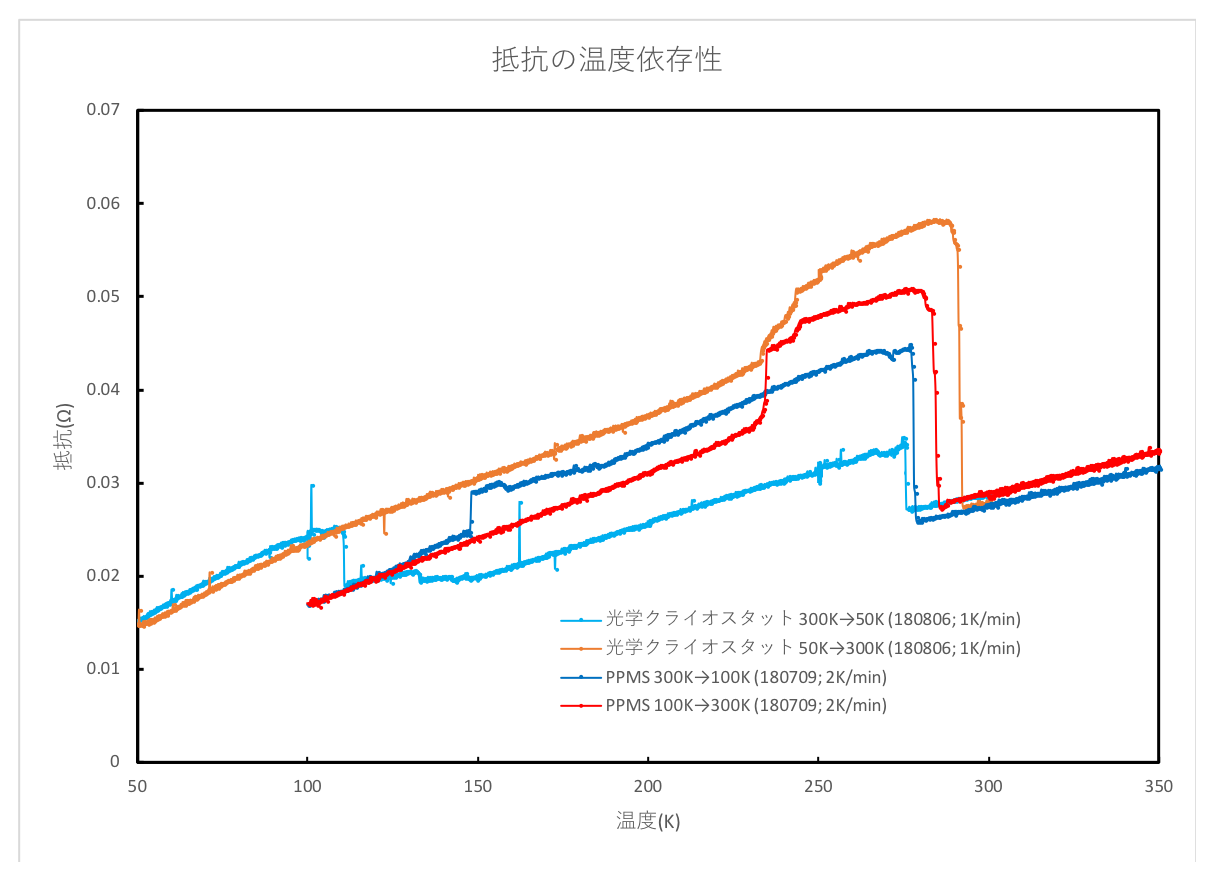
\includegraphics[width=150mm]{PPMS.eps}
  \end{center}
  \caption{PPMS実験と抵抗値の比較}
  \label{fig:PPMS}
\end{figure}
 
\subsection{偏光顕微光学系}
付録\ref{seq:BS_characterization}に示すように、本実験光学系で非偏光ビームスプリッタ(Thorlabs社製\#BSW41-532)を透過または反射する光には偏光に依存して位相差がつく。その偏光に依存した位相差に起因して、ビームスプリッタを透過または反射する光の偏光状態は変化する。例えば直線偏光をビームスプリッタに入射しても、透過する光は楕円偏光になってしまう。このような入射光の偏光状態の変化を避けるため、これまでビームスプリッタにp偏光(偏光が鉛直方向)かs偏光(偏光が水平方向)、無偏光のみを入射する条件で実験を行ってきた。しかし、結晶の対称性を明らかにするためには、入射光の偏光をより自由に制御する必要がある。図\ref{fig:microscope2}のように1/2波長板をビームスプリッタと対物レンズの間に置けば、ビームスプリッタにp偏光とs偏光のみを入射しながら、試料に入射する光の偏光をビームスプリッタより後方で制御することができる。この光学系を用いて入射光の偏光をより高い自由度で制御し、低温相の理解を深めることが今後の課題である。
\begin{figure}[p]
  \begin{center}
   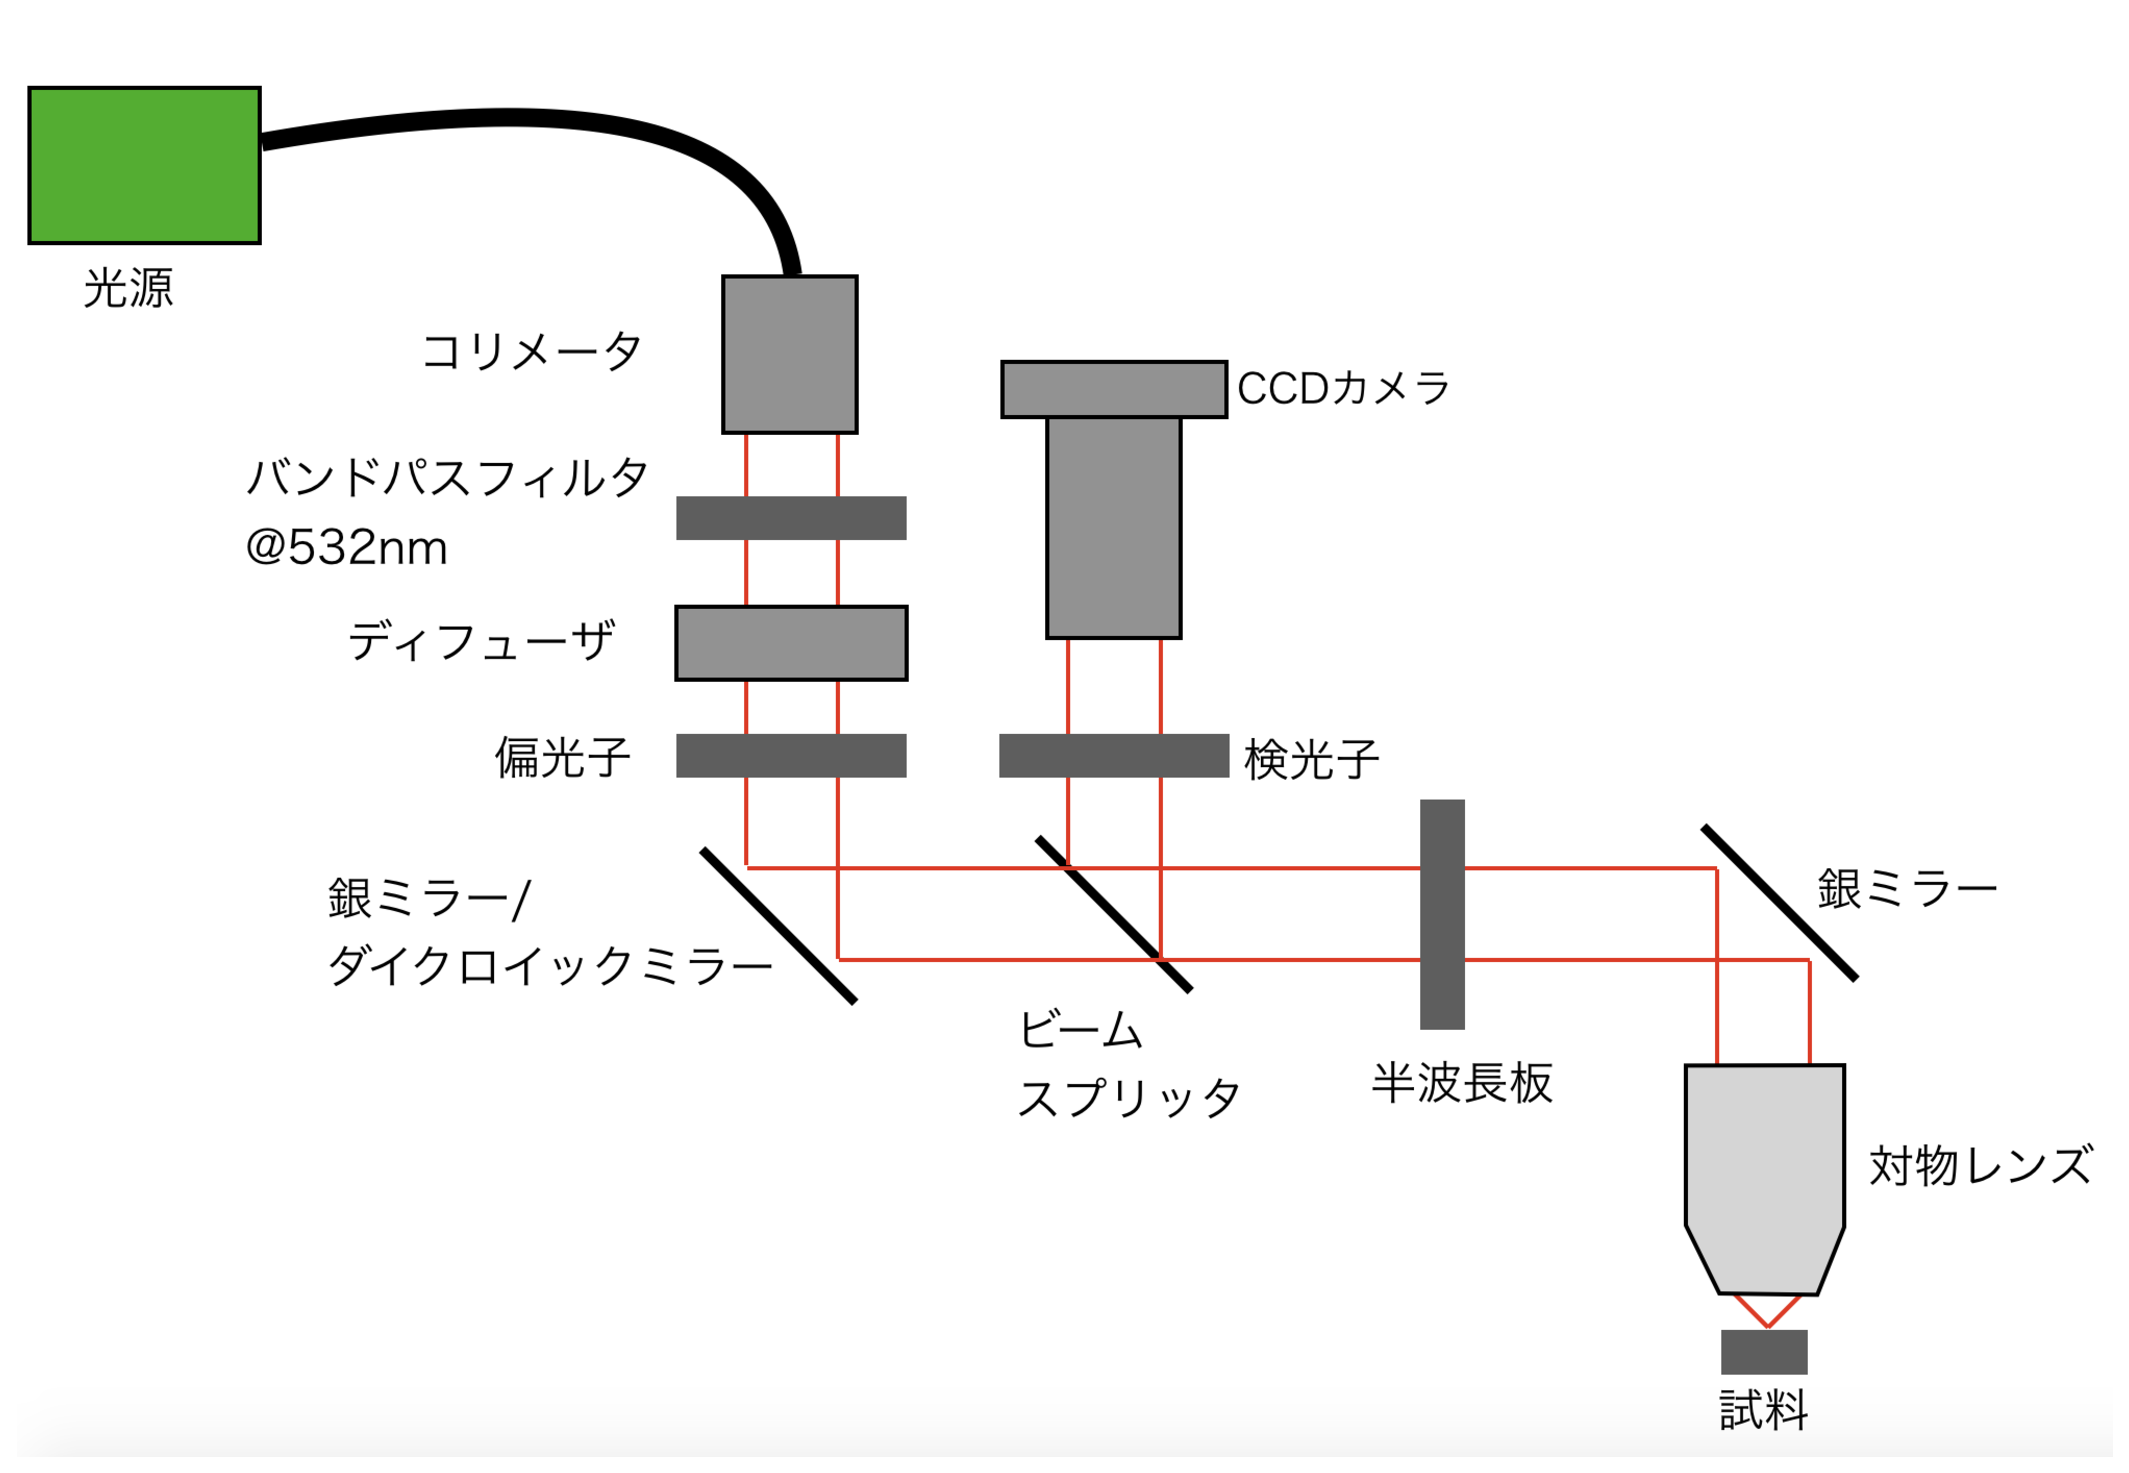
\includegraphics[width=120mm]{microscope2.eps}
  \end{center}
  \caption{改良された偏光顕微光学系の模式図}
  \label{fig:microscope2}
\end{figure}



\section{結論}
筆者は2018年前期の実験において、バルクIrTe$_2$試料を温度変化させながら偏光顕微鏡で観察した。
300Kから除冷してゆくと偏光顕微鏡写真から、280K付近で異方性のある相が現われ、さらに110K付近で異なった相が現れることを確認した。バルクIrTe$_2$試料が280K付近と110K付近で2回相転移したことを強く示唆する結果だと本報告書の筆者は考える。これまでの実験で得られた知見から光学系を改良し、今後結晶の相をより明らかに同定できるように実験を進めていきたい。


%\section{謝辞}
\newpage
\appendix
\section{顕微光学系に関して}
\subsection{光源とディフューザー}
本実験には白熱電球を用いた光源を用いた。この光源からの光はそのままでは拡散するので、ファイバーを通してコリメータで平行光に直した。この平行光をビームスプリッタや対物レンズ等を通して試料に入射したところ、図\ref{fig:without_diffuser}のようにまだら模様(スペックルパターン)が見て取れた。
この模様は入射光がコヒーレンスにより干渉してできるものである。この模様の効果を抑えるためには入射光の空間コヒーレンスを小さくする工夫が効果的である。

筆者は入射光のコヒーレンスを小さくするため光学系にEdmund社製のホログラフィックディフューザー(\#47-991/拡散角度$1^\circ$)を導入した。その結果、図\ref{fig:with_diffuser}のように入射光強度の一様な分布が得られた。
キムワイプの切れ端を光路中に挿入しても同様の効果が得られるが、強度が大きく落ち込んでしまい拡散角も大きいことに注意する。
\begin{figure}[p]]
 \begin{minipage}{0.5\hsize}
  \begin{center}
   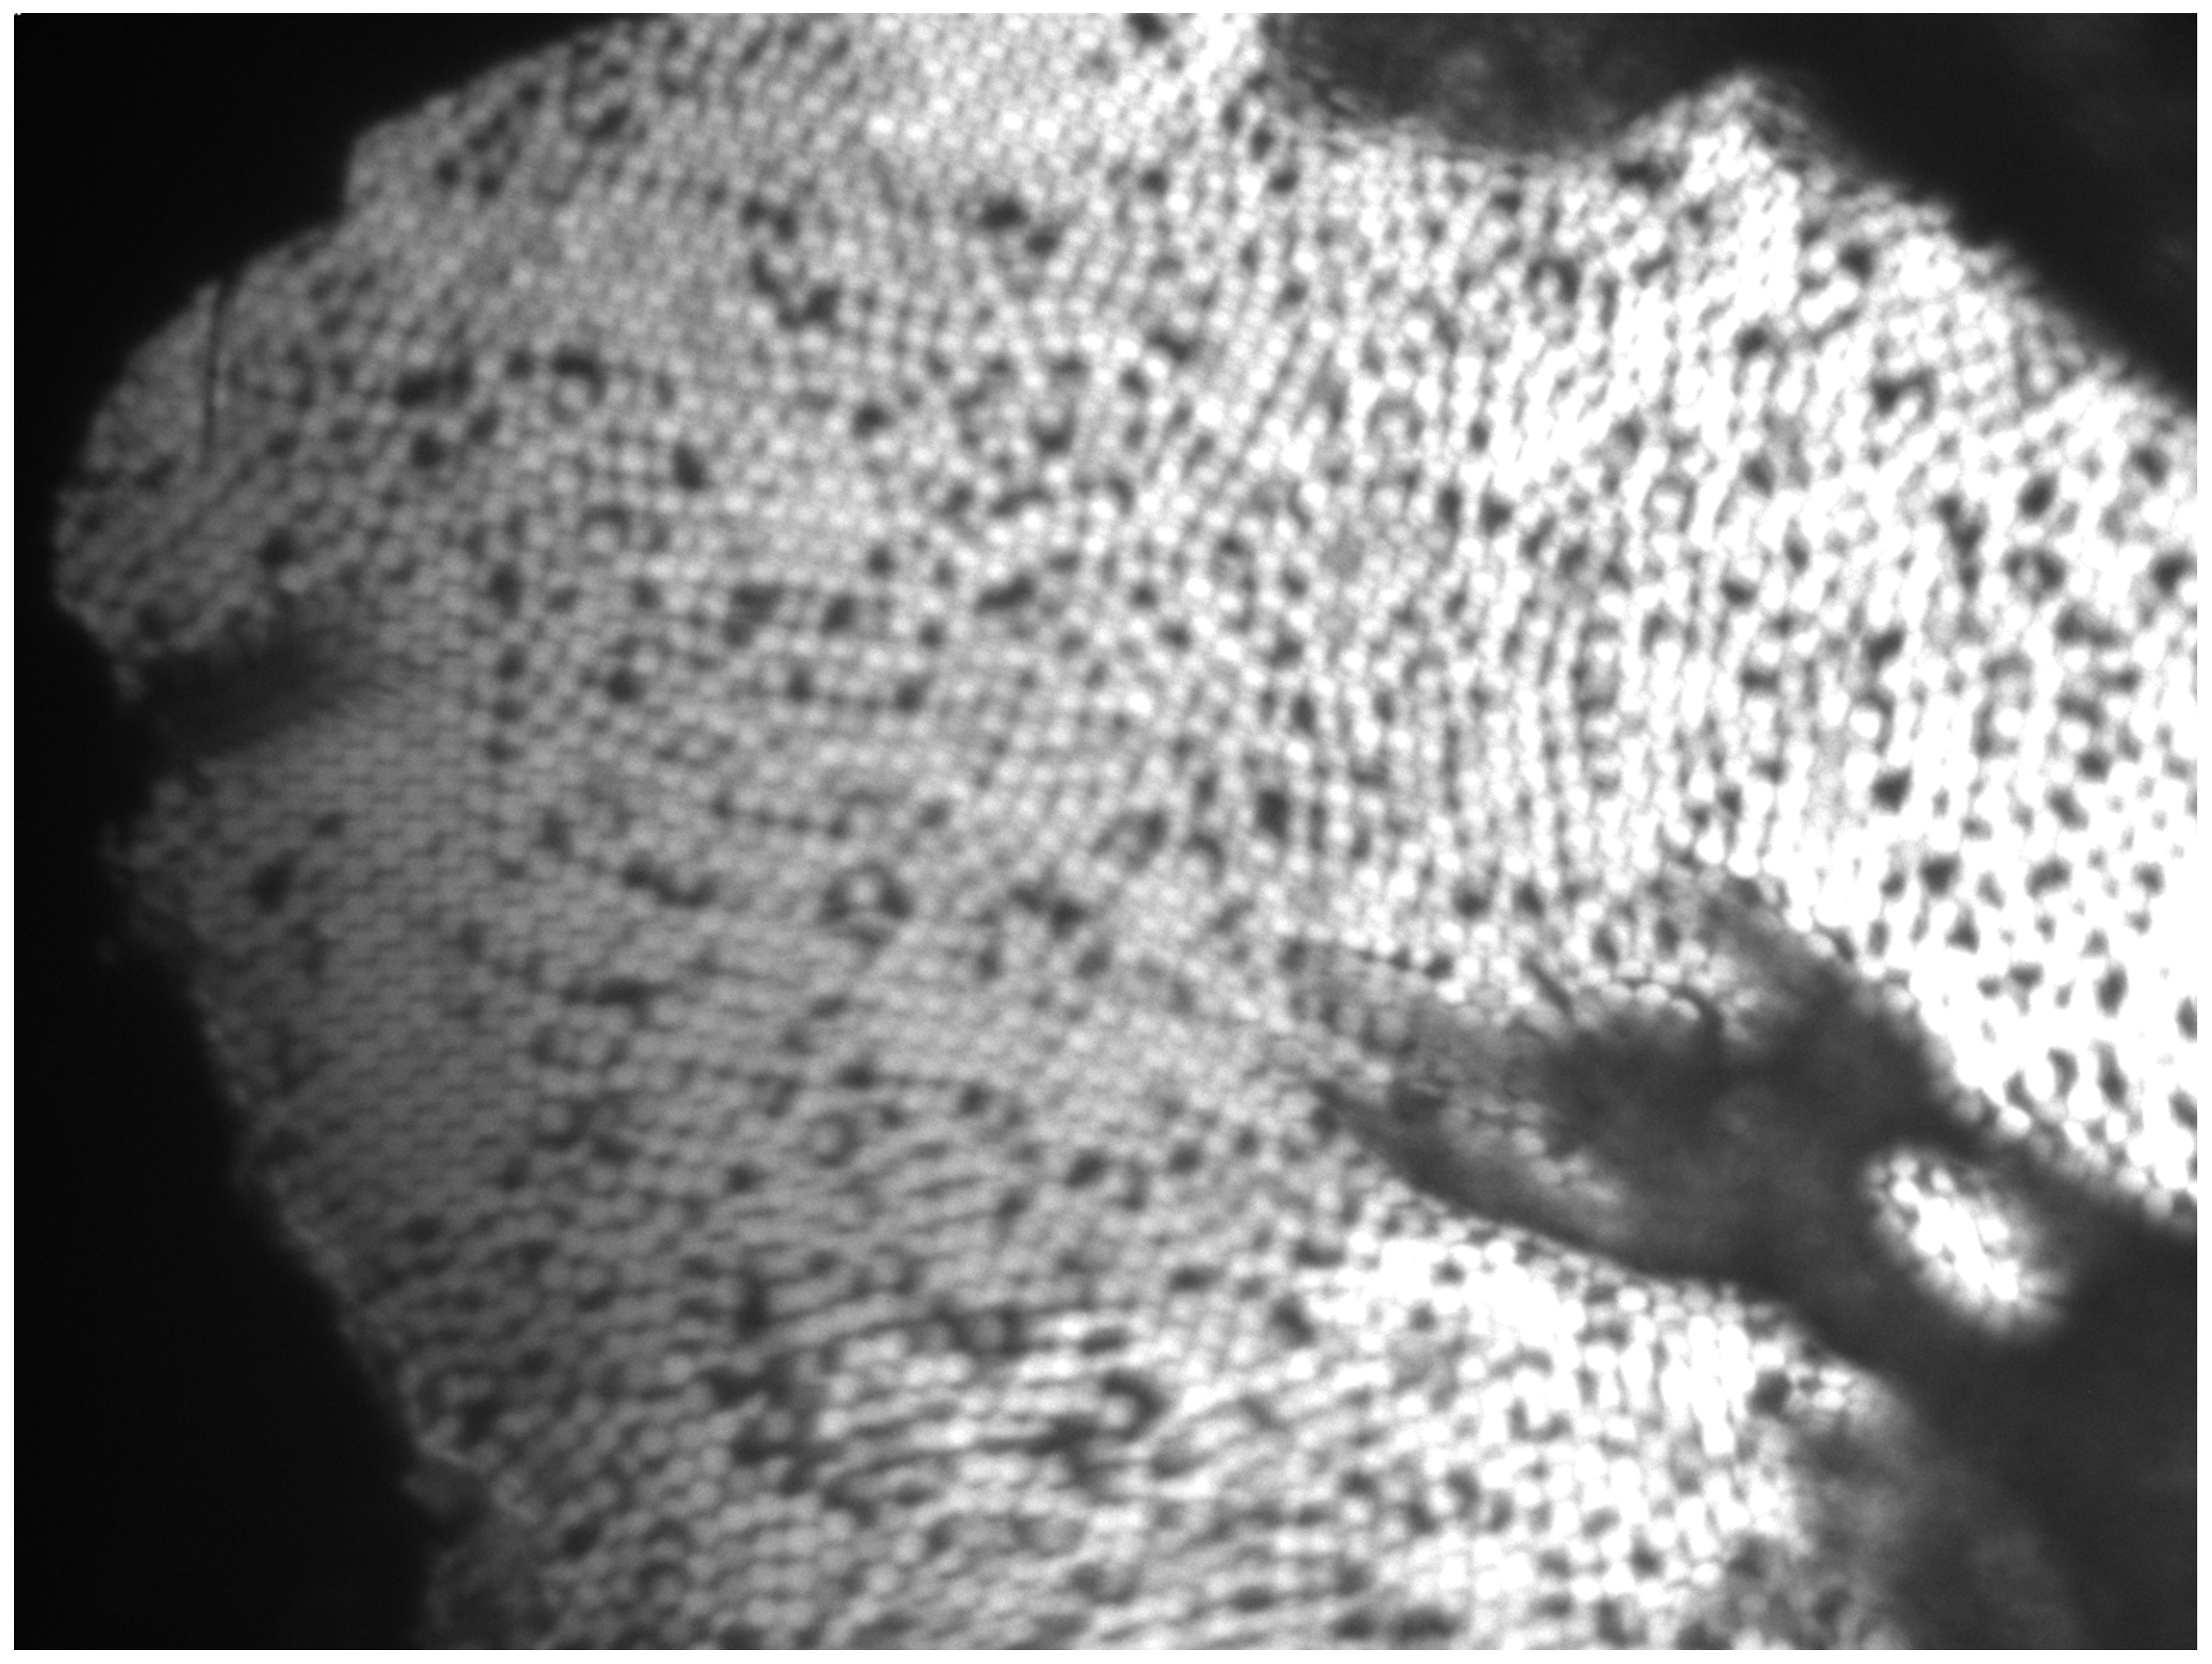
\includegraphics[width=70mm]{without_diffuser.eps}
  \end{center}
  \caption{ディフューザーなし}
  \label{fig:without_diffuser}
 \end{minipage}
 \begin{minipage}{0.5\hsize}
  \begin{center}
   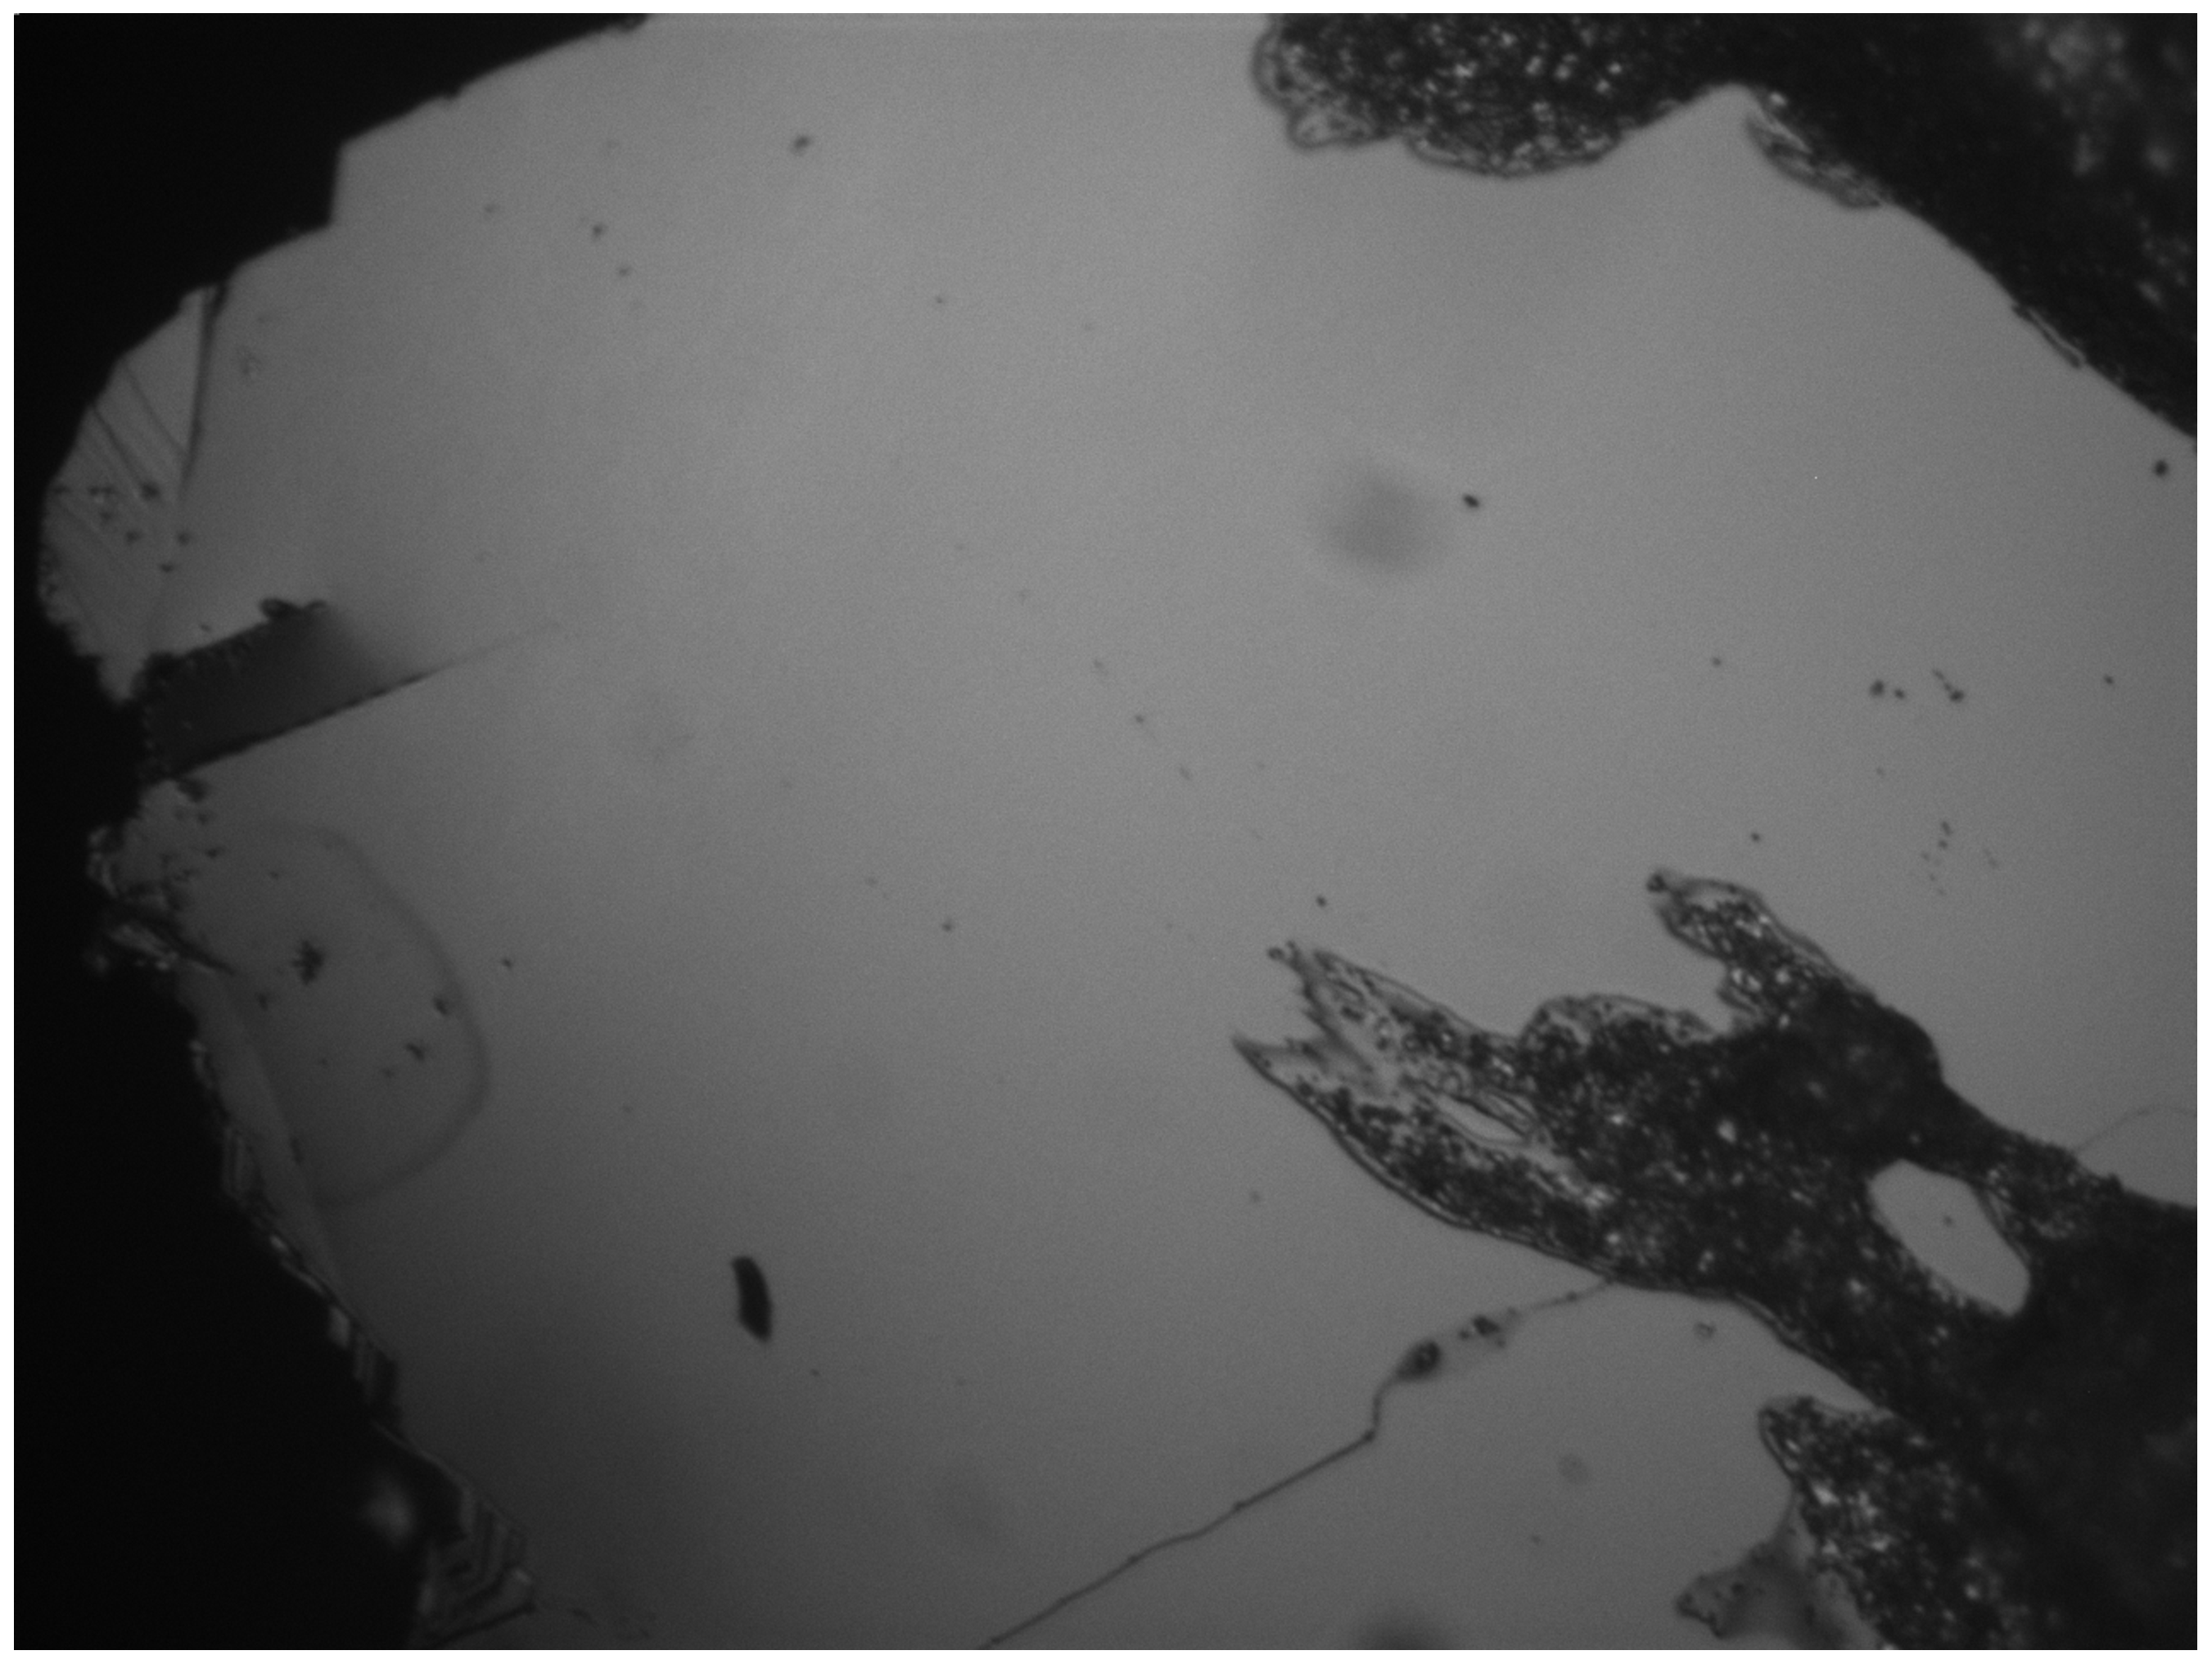
\includegraphics[width=70mm]{with_diffuser.eps}
  \end{center}
  \caption{ディフューザーあり}
  \label{fig:with_diffuser}
 \end{minipage}
\end{figure}

\subsection{非偏光ビームスプリッタの偏光依存性の評価}
\label{seq:BS_characterization}
本節では非偏光ビームスプリッタ(Thorlabs社製\#BSW41-532)の、偏光依存性に関して議論する。

まずビームスプリッタを光が透過する場合に関して、p偏光の透過率とs偏光の透過率を独立に評価し、さらにp偏光の透過光とs偏光の透過光の間についた位相差を評価した。
そのために図\ref{fig:schematics_BS_T2}のような光学系を構成した。光源側の偏光子の偏光軸は鉛直方向と水平方向、鉛直方向に対して45度傾けた角度にとった。偏光軸の角度それぞれに対して検光子を回転させながら、CCDに入る信号の平均強度をプロットしたものが図\ref{fig:BS_T2}である(データ点)。さらにデータ点からビームスプリッタのp偏光の透過率$t_p$とs偏光の透過率$t_s$、p偏光とs偏光の間につく位相差$\phi_t$を推定した。推定は非線形最小二乗法により、解析にはMicrosoft社Excelのソルバーを用いた。その推定した$t_p,t_s,\phi_t$を用いてデータ点をフィッティングした曲線を図\ref{fig:BS_T2}に示す。
p偏光の透過率とs偏光の透過率の比は$t_p/t_s=1.10$で、p偏光とs偏光の間につく位相差は$\phi_t=147^\circ$と推定した。

次にビームスプリッタで光が反射される場合に関しても同様に、p偏光の反射率とs偏光の反射率、p偏光とs偏光の反射光の間についた位相差を評価した。
そのために図\ref{fig:schematics_BS_R}のような光学系を構成した。光源側の偏光子の偏光軸は鉛直方向と水平方向、鉛直方向に対して45度傾けた角度にとった。偏光軸の角度それぞれに対して検光子を回転させながら、CCDに入る信号の平均強度をプロットしたものが図\ref{fig:BS_R}である(データ点)。さらにデータ点に対して、p偏光の反射率$r_p$とs偏光の反射率$r_s$、p偏光とs偏光の間につく位相差$\phi_r$を推定した。推定した$r_p,r_s,\phi_r$を用いたデータ点をフィッティングした曲線を図\ref{fig:BS_R}に示す。
p偏光の透過率とs偏光の透過率の比は$r_p/r_s=1.04$で、p偏光とs偏光の間につく位相差は$\phi_r=24^\circ$と推定した。

最後に図\ref{fig:schematics_BS_T2R}のように、透過と反射が一度ずつあるような光学系で、p偏光の透過率と反射率の積、s偏光の透過率と反射率の積、p偏光とs偏光の間についた位相差を評価した。光源側の偏光子の偏光軸は鉛直方向と水平方向、鉛直方向に対して45度傾けた角度にとった。偏光軸の角度それぞれに対して検光子を回転させながら、CCDに入る信号の平均強度をプロットしたものが図\ref{fig:BS_T2R}である(データ点)。また図\ref{fig:BS_T2R}には、偏光子を取り外した状態で検光子を回転させて信号強度を測定したデータもプロットしてある。データ点に対して、p偏光の透過率と反射率の積$t_pr_p$とs偏光の透過・反射率$t_sr_s$、p偏光とs偏光の間につく位相差$\phi$を推定した。推定した$t_pr_p,t_sr_s,\phi$を用いたデータ点をフィッティングした曲線を図\ref{fig:BS_R}に示す。
p偏光の透過率とs偏光の透過率の比は$t_pr_p/(t_sr_s)=0.99$で、p偏光とs偏光の間につく位相差は$\phi_t=24^\circ$と推定した。

非偏光ビームスプリッタに関して評価した結果を表\ref{tab:BS}にまとめる。

\begin{table}[htb]
  \begin{tabular}{lcrr}
     & 透過 & 反射  & 透過・反射 \\
    透過・反射率の比 & 1.10 & 1.04 & 0.99\\
    位相差($^\circ$) & 147 & 24 &138
    \label{tab:BS}
  \end{tabular}
\end{table}

\begin{figure}[p]
     \begin{minipage}{\hsize}
  \begin{center}
   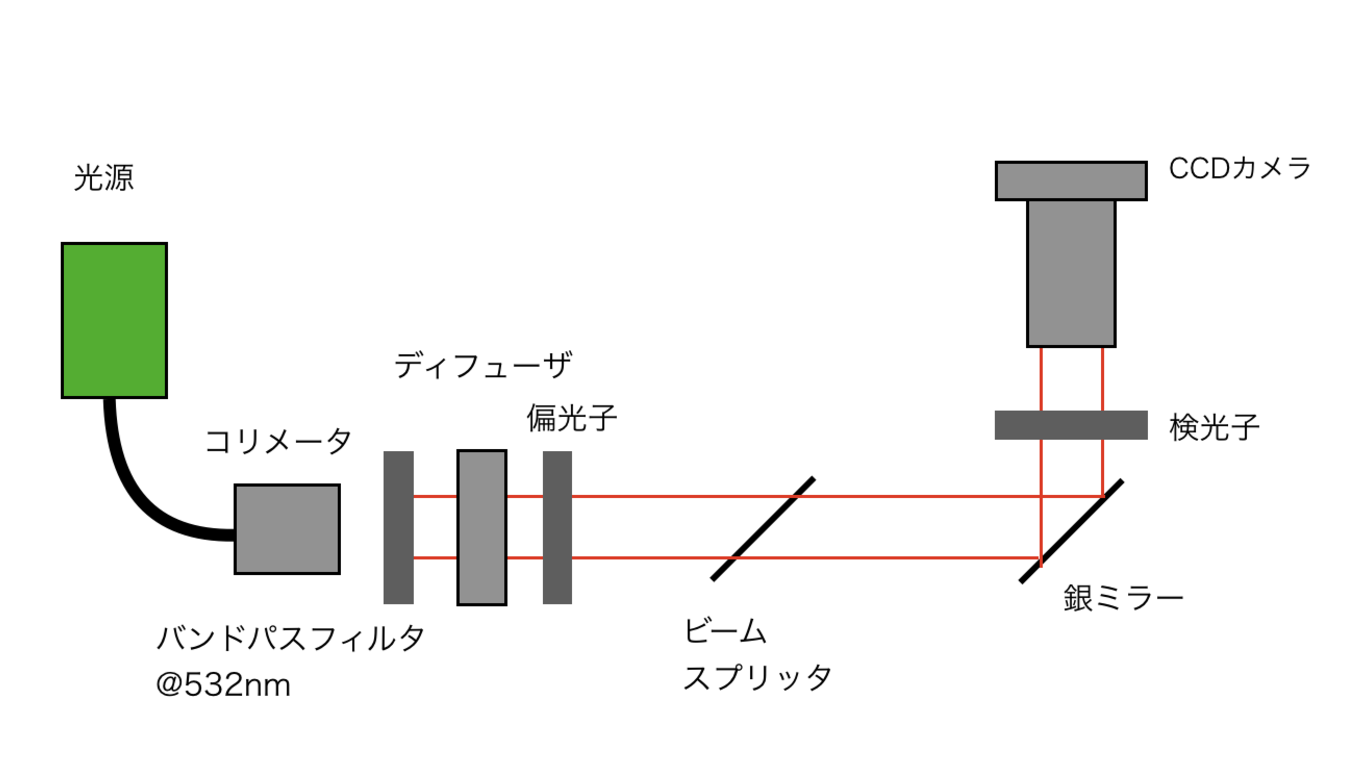
\includegraphics[width=120mm]{schematics_BS_T2.eps}
  \end{center}
  \caption{ビームスプリッタを評価する光学系(透過)}
  \label{fig:schematics_BS_T2}
   \end{minipage}
  \begin{minipage}{\hsize}
  \begin{center}
   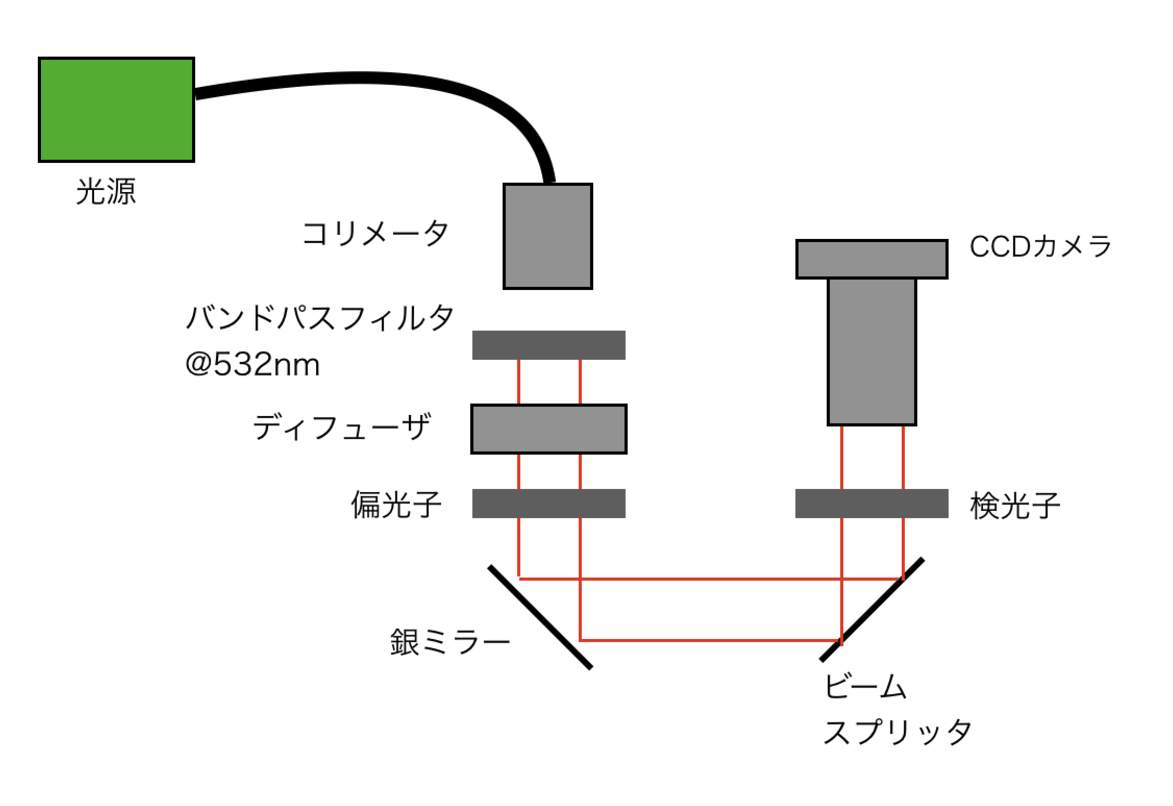
\includegraphics[width=110mm]{schematics_BS_R.eps}
  \end{center}
  \caption{ビームスプリッタを評価する光学系(反射)}
  \label{fig:schematics_BS_R}
   \end{minipage}
     \begin{minipage}{\hsize}
  \begin{center}
   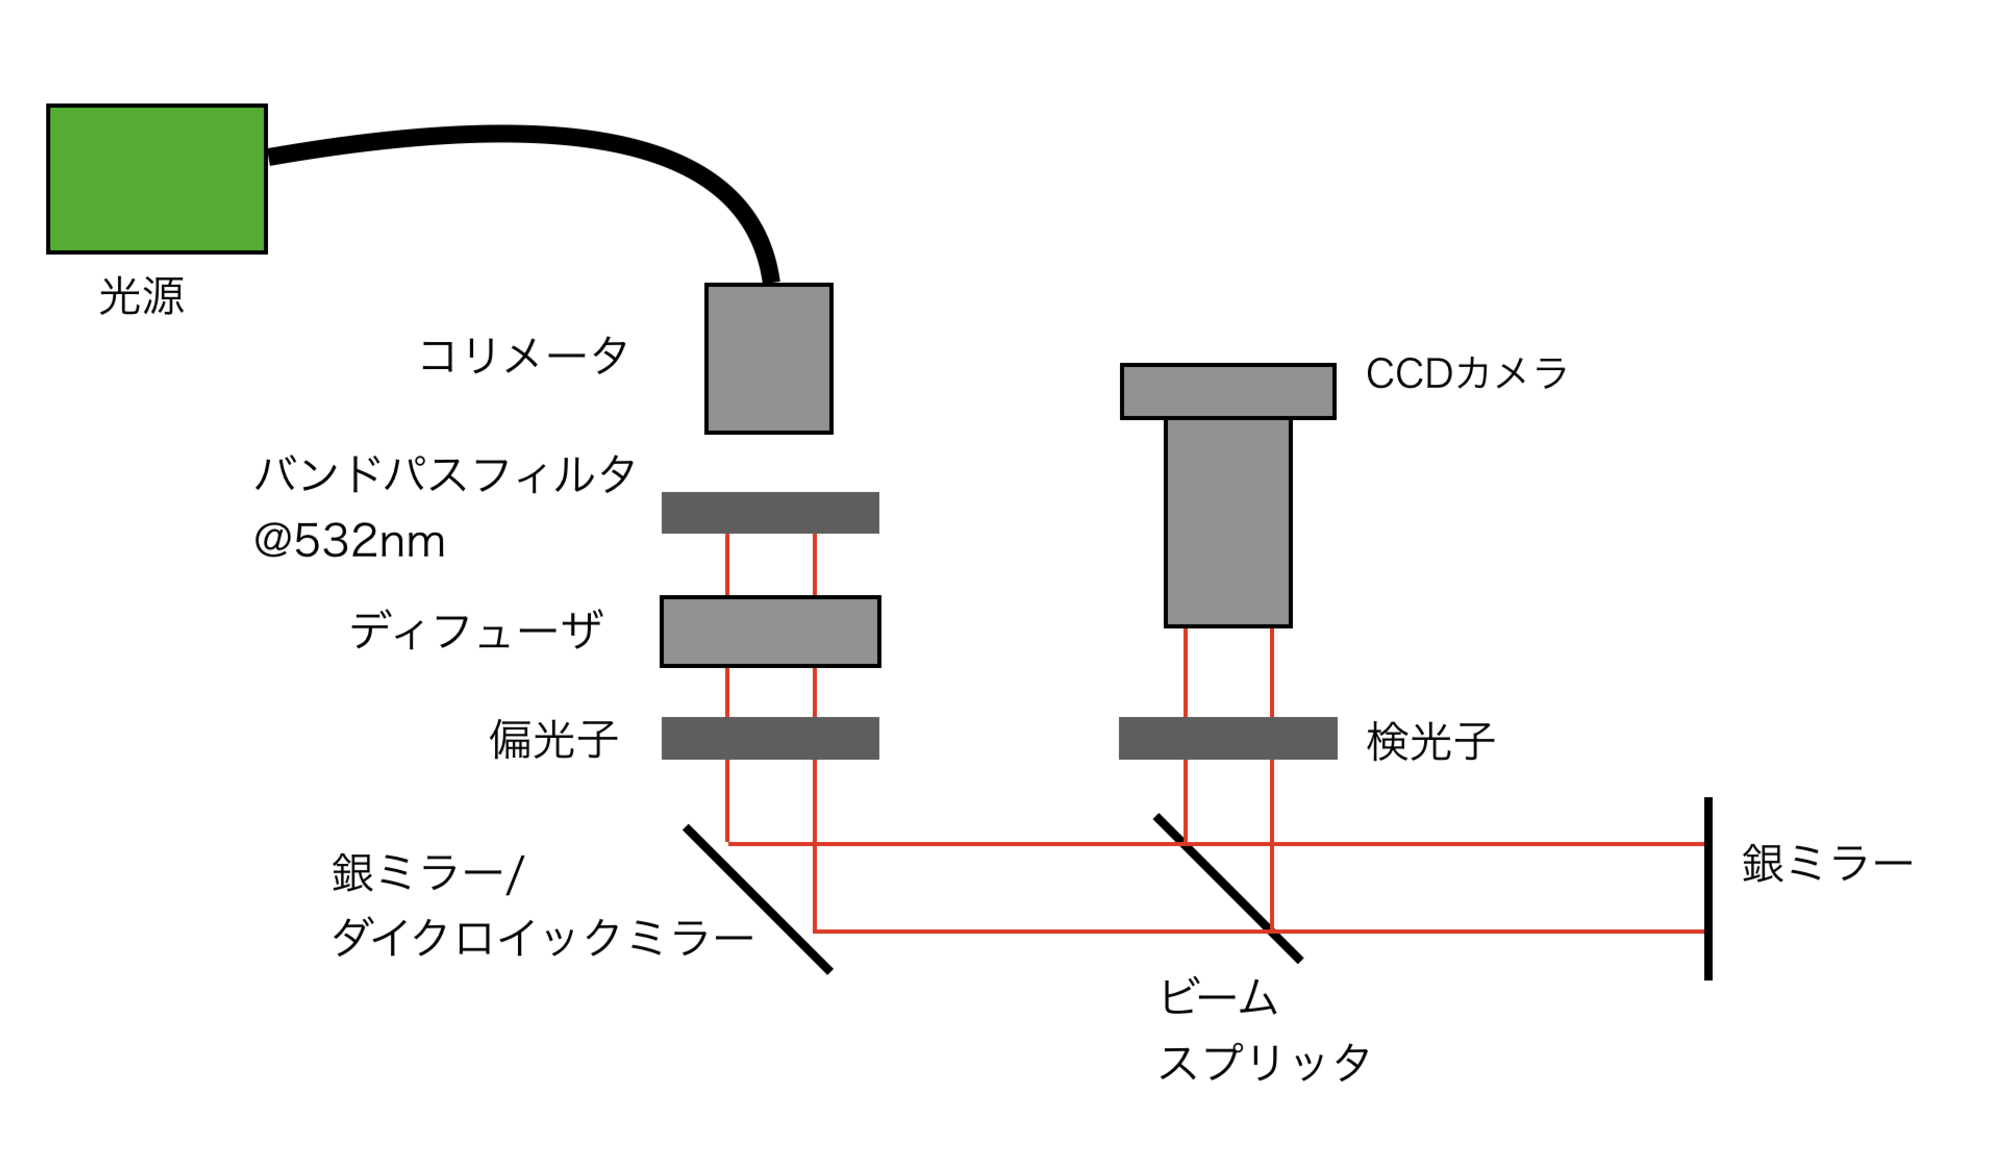
\includegraphics[width=120mm]{schematics_BS_T2R.eps}
  \end{center}
  \caption{ビームスプリッタを評価する光学系(透過・反射)}
  \label{fig:schematics_BS_T2R}
   \end{minipage}
\end{figure}

\begin{figure}[p]
    \begin{minipage}{\hsize}
  \begin{center}
   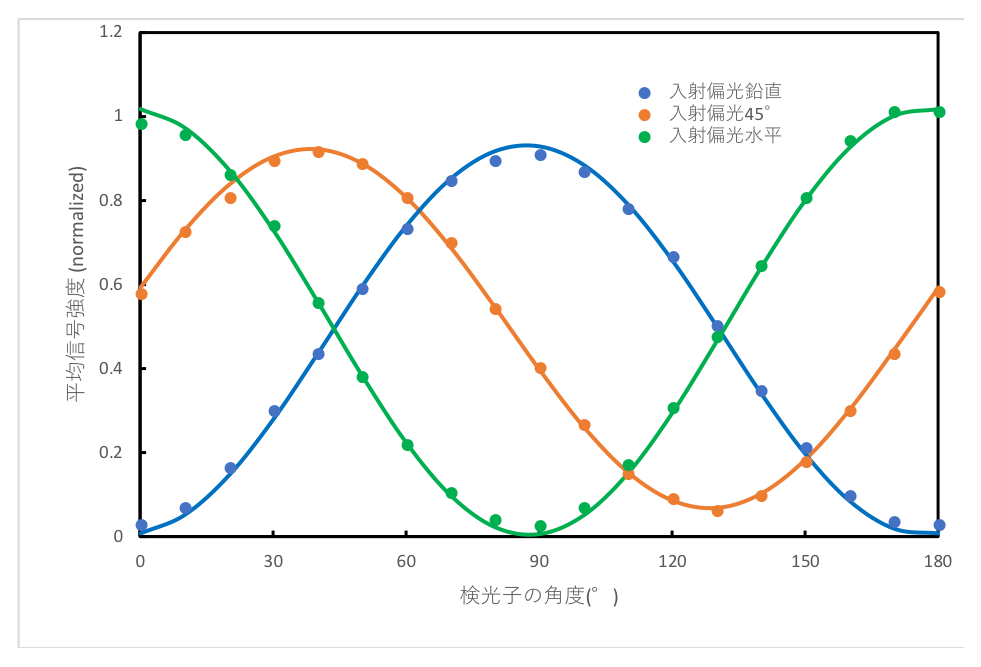
\includegraphics[width=0.7\hsize]{BS_T2.eps}
  \end{center}
  \caption{ビームスプリッタの偏光依存性(透過)}
  \label{fig:BS_T2}
   \end{minipage}
    \begin{minipage}{\hsize}
  \begin{center}
   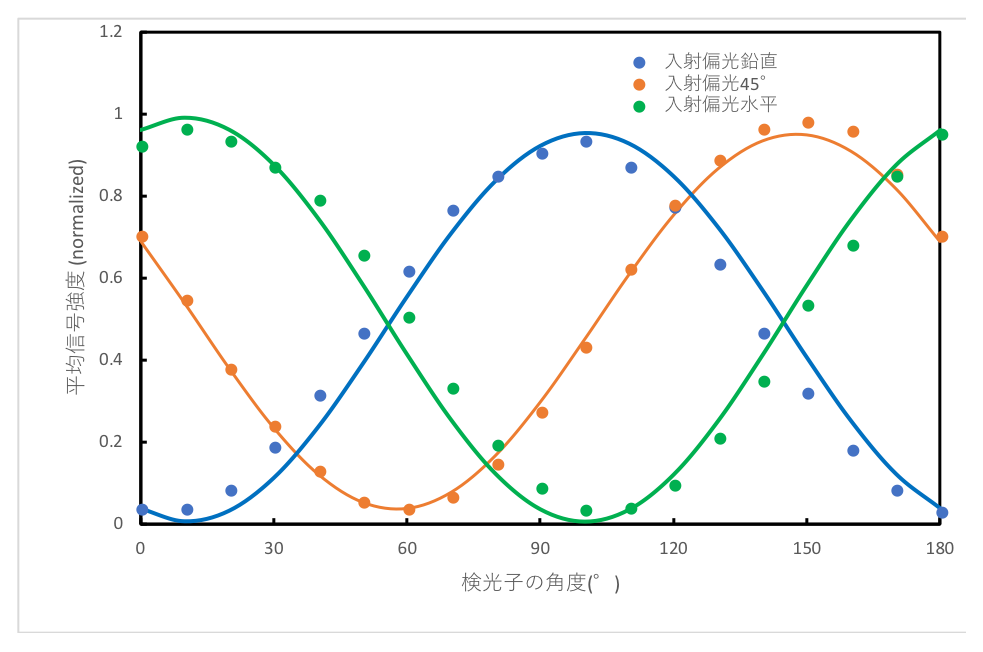
\includegraphics[width=0.7\hsize]{BS_R.eps}
  \end{center}
  \caption{ビームスプリッタの偏光依存性(反射)}
  \label{fig:BS_R}
   \end{minipage}
    \begin{minipage}{\hsize}
  \begin{center}
   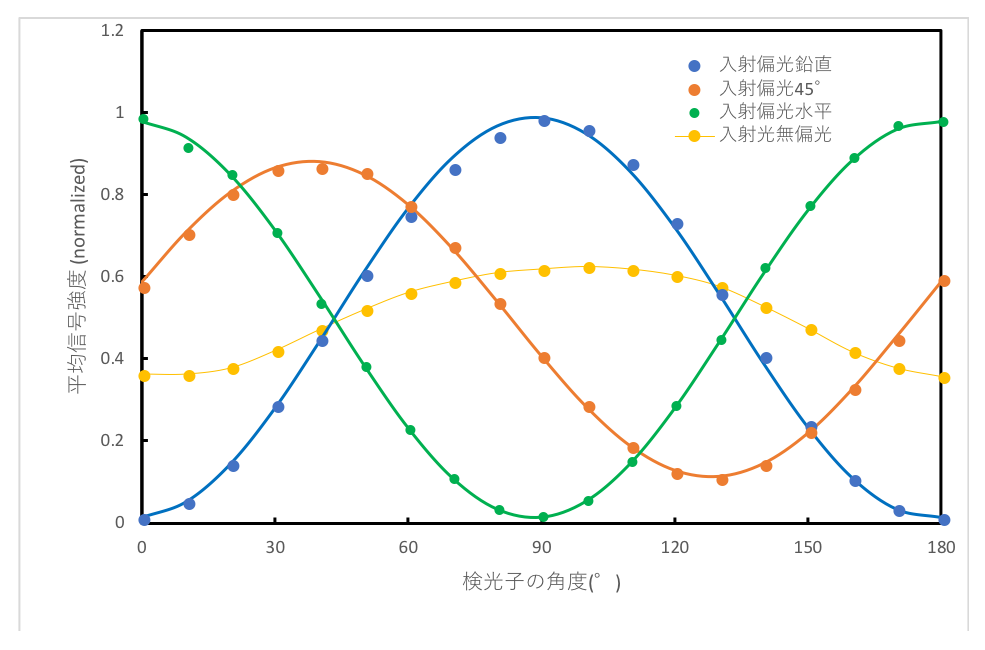
\includegraphics[width=0.7\hsize]{BS_T2R.eps}
  \end{center}
  \caption{ビームスプリッタの偏光依存性(透過・反射)}
  \label{fig:BS_T2R}
   \end{minipage}
\end{figure}


\subsection{顕微光学系の実効的な消光比について}
図\ref{fig:microscope}の光学系で試料の代わりに銀ミラーを置き、偏光子と検光子を垂直に配置したときの信号強度と平行に配置したときの信号強度をそれぞれ測定して、その比(実効的な消光比と呼ぶ)をとるとたかだか10程度だった。すなわち現状の光学系では直交偏光の条件でも、平行偏光の信号成分を精度よく取り除けていない。このとき、直交偏光で試料を顕微鏡像を撮影しても、強度の大きな平行偏光からの寄与がのってしまい、結晶の異方性を観察するのに都合が悪い。

本実験で用いたガラス偏光フィルター(Edmund製\#43-786)は波長532nmで消光比15000程度である。したがって現状で平行偏光の成分を取り除けていないのは、主にビームスプリッタと対物レンズの特性に起因すると筆者は考える。

まずビームスプリッタの寄与に関して述べる。付録\ref{seq:BS_characterization}の結果から、ビームスプリッタ(Thorlabs社製\#BSW41-532)を透過したp偏光とs偏光には位相差がついてしまう。筆者のこれまでの実験では、偏光子の偏光軸を精度よく鉛直・水平方向に出していなかった。実際に付録\ref{seq:BS_characterization}の非線形最小二乗法による解析では、偏光子の偏光軸のアライメントに5度程度の誤差があった可能性が示唆された。 したがってp偏光を入射したつもりでも、実際はビームスプリッタにはp偏光からわずかに傾いた光が入射され、楕円偏光がビームスプリッタから出力されていた。この光学系のアライメントのずれに起因して、顕微光学系の実効的な消光比が小さくなってしまった可能性がある。偏光子の偏光軸を精度よく水平・鉛直方向に出すには、反射率が偏光に依存するビームスプリッタ(Thorlabs製\#BSW-26)で反射される光をCCDで検出し、その結果を解析することが効果的だと筆者は考える。このような偏光子のアライメント方法の改良のもとで、顕微光学系の実効的な消光比はいくらか改善することが見込まれる。

次に顕微光学系の実効的な消光比に対する対物レンズの寄与を評価する実験を行なった。図\ref{fig:microscope}の光学系で試料の代わりに銀ミラーを置き、光源側の偏光子の偏光軸は鉛直方向と水平方向、鉛直方向に対して45度傾けた角度にとった。偏光軸の角度それぞれに対して検光子を回転させながら、CCDに入る信号の平均強度をプロットしたものが図\ref{fig:objective_2}である。図\ref{fig:BS_T2R}のデータを取得した時と比較して、対物レンズを光学系に挿入している点のみが異なる。
対物レンズを挿入しなかったとき(図\ref{fig:BS_T2R})の消光比は73程度だったが、対物レンズ(Mitsutoyo製M Plan Apoシリーズ/倍率x10)を挿入したとき(図\ref{fig:objective_2})の消光比は10程度だった。したがって対物レンズを挿入することで、偏光顕微光学系の実効的な消光比は大きく損なわれることが分かった。

対物レンズを挿入したことで消光比が落ち込む理由は、対物レンズの光軸から離れたところを通る光の一部が偏光方向を回転してしまうことにある。対物レンズの光軸から離れたところで光軸と平行に進む光はレンズの曲面に対して斜めに入射する。斜め入射する光の透過率は偏光に依存するため、透過光の偏光は回転する。また透過率が偏光に依存せず100\%だと仮定しても、対物レンズの光軸から離れたところを通る光の光路は曲げられるため、一般に偏光の方向も変わってしまう。これらの効果により直線偏光を対物レンズに入射しても、集光されて出てくる光の偏光状態は空間的に異なった分布を持つ。対物レンズを用いる現状の光学系で、このような効果の影響を完全に排除することはできない。しかし入射光を対物レンズの光軸付近のみに通し、光軸付近を通った反射光のみ検出すれば、影響を小さくできる。すなわち照明光を空間的に絞ってビームサイズを小さくし、さらに対物レンズの光軸付近を通っってきた反射光のみを検出する工夫が消光比を改善するために効果的である。この工夫は光学系にアイリスを挿入することで簡単に実現できる。すなわち図\ref{fig:microscope3}のような偏光光学系を構成すれば、対物レンズに起因する消光比の悪化を軽減することができると筆者は考える。


\begin{figure}[p]
  \begin{center}
   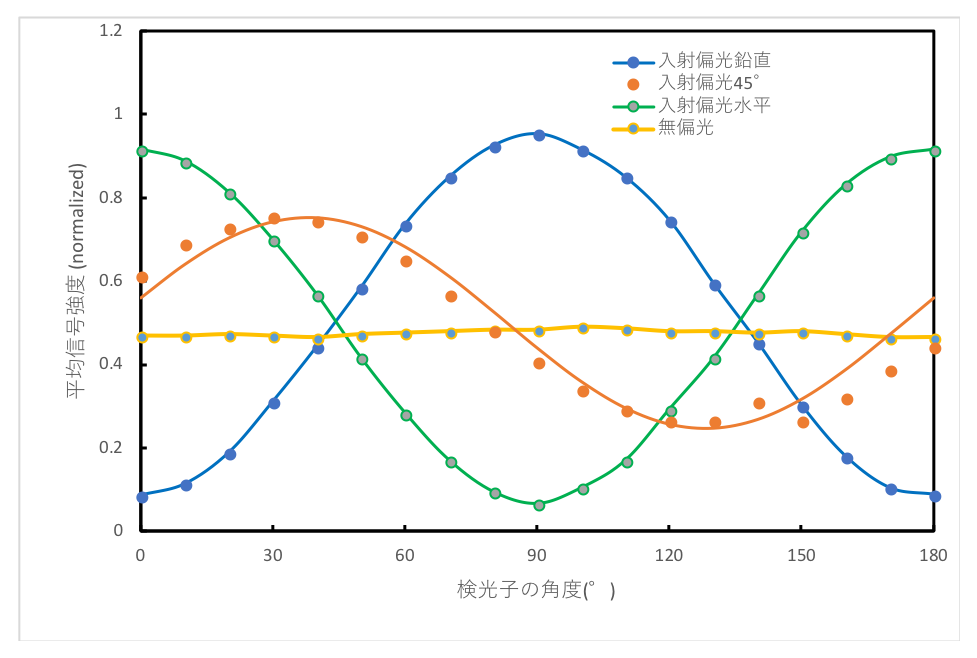
\includegraphics[width=120mm]{objective_2.eps}
  \end{center}
  \caption{顕微光学系の偏光依存性}
  \label{fig:objective_2}
\end{figure}

\begin{figure}[p]
  \begin{center}
   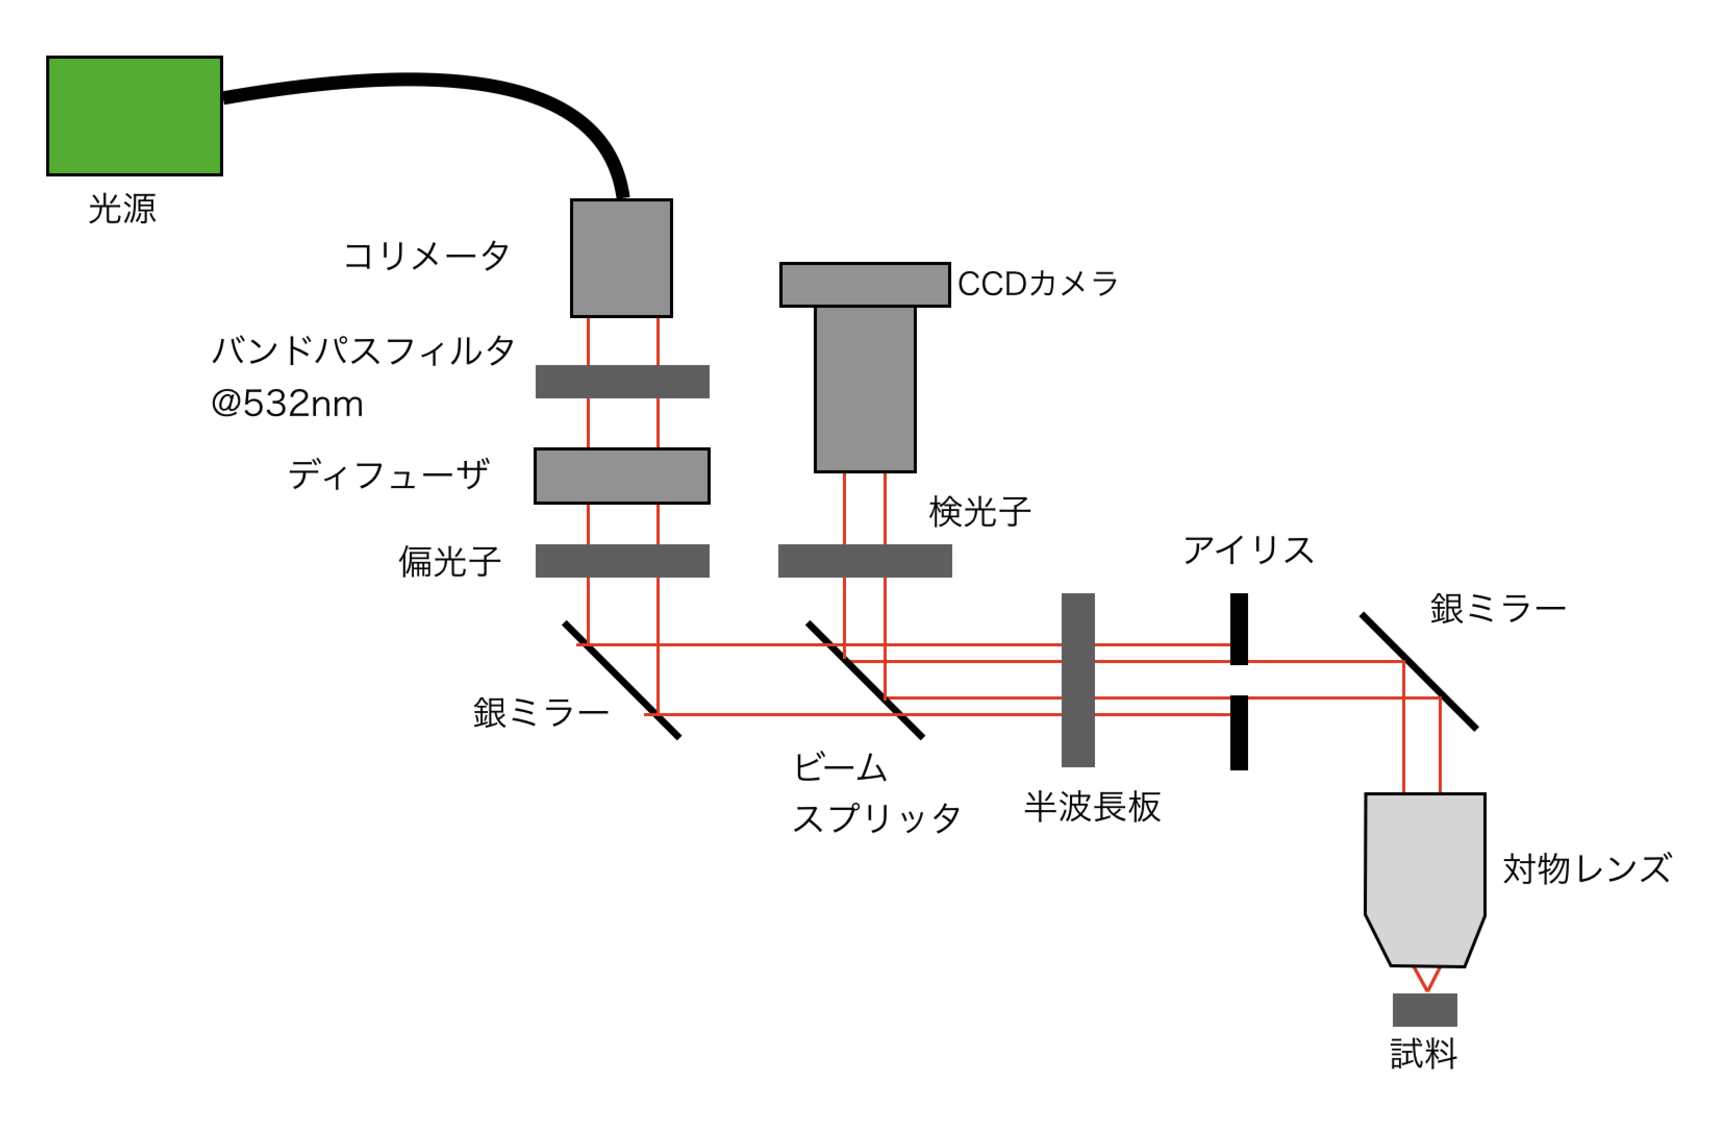
\includegraphics[width=120mm]{microscope3.eps}
  \end{center}
  \caption{改良された偏光顕微光学系の模式図}
  \label{fig:microscope3}
\end{figure}

\section{異方性のある反射率}
\subsection{一般の場合の反射率の導出}
比誘電率テンソル$\epsilon$が与えられたときの複素反射率テンソル$r$を導く。導出は文献\cite{dielectric_tensor_triclinic}に従う。

まず結晶の内部をz方向に伝搬する電磁波に関して考える。
結晶中のMaxwell方程式は真空の透磁率$\mu_0$と真空の誘電率$\epsilon_0$、比誘電率テンソル$\epsilon$を用いて、以下のように書ける。だだし結晶は磁性を持たず、電流密度と電荷密度がいたるところ0であるとした。
\begin{eqnarray}
\label{H1}
\mu_0 \nabla \cdot {\bf H} &=& 0,\\
\label{E1}
\nabla \times {\bf E} &=& -\mu_0 \frac{\partial \bf H}{\partial t},\\
\label{E2}
\epsilon_0 \nabla \cdot  (\epsilon {\bf E}) &=& 0,\\
\label{H2}
\nabla \times {\bf H} &=& \epsilon_0 \epsilon  \frac{\partial \bf E}{ \partial t}.
\end{eqnarray}

式\ref{E1}と式\ref{H2}をフーリエ変換すると、
\begin{eqnarray}
\label{E3}
{\bf k} \times {\bf E} = \mu_0 \omega {\bf H},\\
\label{H3}
{\bf k} \times {\bf H} = -\epsilon_0 \omega  \epsilon  {\bf E}.
\end{eqnarray}

式\ref{E3}に式\ref{H3}を代入してベクトル解析の公式を用いると、$k_0=\omega \sqrt{\epsilon_0 \mu_0}$を自由空間の波数として、
\begin{eqnarray}
\label{kk}
k^2 {\bf E} - ( {\bf k} \cdot {\bf E} ) {\bf k}=  k_0^2  \epsilon {\bf E}.
\end{eqnarray}

電磁波はz方向に伝搬するので、$k_x=k_y=0, k_z=k$である。式\ref{kk}から以下が言える。
\begin{eqnarray}
\label{eE}
\left(
    \begin{array}{ccc}
      \epsilon_{xx}-p & \epsilon_{xy} & \epsilon_{xz} \\
      \epsilon_{yx} &  \epsilon_{yy} -p & \epsilon_{yz} \\
      \epsilon_{zx} & \epsilon_{zy} & \epsilon_{zz} \\
    \end{array}
\right)
\left( \begin{array}{c} E_x\\ E_y\\ E_z \\ \end{array} \right)
=\left( \begin{array}{c} 0\\ 0\\ 0 \\ \end{array} \right).
\end{eqnarray}
ただし$p=k^2/k_0^2$はz方向の(複素)屈折率の二乗である。この式が零ベクトルでない電場$E$に関して成り立つとき左辺の行列は非正則で行列式は0である。行列式を0に等置した$p$に関する二次方程式を解くと、$p$は以下の$p^+$と$p^-$の二つの値をとる。
\begin{eqnarray}
p^\pm = (\frac{k^\pm}{k_0})^2 =\frac{1}{2u}[v \pm \sqrt{v^2-4uw}].
\end{eqnarray}
ただし、$u,v,w$を以下のようにおいた。
\begin{eqnarray}
u &=& \epsilon_{zz},\\
v &=& (\epsilon_{xx}+\epsilon_{yy})\epsilon_{zz} -\epsilon_{xz}^2-\epsilon_{yx},\\
w &=& \epsilon_{xx}\epsilon_{yy}\epsilon_{zz}-\epsilon_{xx}\epsilon_{yx}^2-\epsilon_{yy}\epsilon_{zx}^2 -\epsilon_{zz}\epsilon_{xy}^2 +2\epsilon_{xy}\epsilon_{yz}\epsilon_{zx}.
\end{eqnarray}

二つの$p^\pm$に対応して式\ref{eE}を満たす電場$E$は二つ存在する。すなわち結晶中をz方向に伝搬する電磁波には二つの異なるモード$E^+$と$E^-$が存在する。$K^\pm$を定数として、
\begin{eqnarray}
E_x^\pm(z) &=& K^\pm [\epsilon_{xy} \epsilon_{yz}- \epsilon_{xz}(\epsilon_{yy}-p^\pm)]exp(-ik^\pm_zz),\\
E_y^\pm(z) &=& K^\pm [\epsilon_{yx} \epsilon_{xz}- \epsilon_{yz}(\epsilon_{xx}-p^\pm)exp(-ik^\pm_zz)],\\
E_z^\pm(z) &=& K^\pm [(\epsilon_{xx}-p^\pm) (\epsilon_{yy}-p^\pm) -\epsilon_{xy}^2]exp(-ik^\pm_zz).
\end{eqnarray}

$E^\pm$を用いて、結晶中の電場$E^{crystal}$と磁場の強さ$H^{crystal}$は以下のように書ける。
\begin{eqnarray}
{\bf E}^{crystal}(z) &=& {\bf E^+(z) + E^-(z) } ,\\
{\bf H}^{crystal}(z) &=& \frac{1}{\mu_0 \omega} {\bf k} \times [{\bf E^+(z) + E^-(z)}].
\end{eqnarray}


以上の結果を用いて光の透過と反射の問題を考える。特に垂直入射の条件を考え、入射光の方向をz軸正の方向にとり結晶表面をxy面にとる。結晶表面に垂直入射した光の波面は表面に平行であるから、反射光と透過光の波面も表面に平行である。すなわち反射光はz軸の負の向き、透過光はz方向の正の向きに伝搬する。

入射光の電場をx方向にとり、その振幅を$E_0$とする。すなわち電場ベクトルは$(E_0,0,0)$である。このとき反射光の電場ベクトルは、複素反射率テンソル$r_{ij}$を用いて、$(r_{xx}E_0, r_{xy}E_0,0)$と書ける。
これから自由空間の電場$E^{free}$と磁場の強さ$H^{free}$は以下で表される。

\begin{eqnarray}
E_x^{free} (z) &=& E_0 exp(-ik_0 z) + r_{xx}E_0 exp(ik_0 z),\\
E_y^{free} (z) &=& r_{xy}E_0 exp(ik_0 z),\\
E_z^{free} (z) &=& 0,\\
{\bf H}^{free}(z) &=& \frac{1}{\mu_0 \omega} {\bf k} \times {\bf E^{free}(z)}.
\end{eqnarray}


結晶表面で電場$E$と磁場の強さ$H$の接線成分が連続であることを境界条件として仮定すると、代数計算から$r_{xx}$と$r_{xy}$に関して以下が言える。
\begin{eqnarray}
r_{xx} &=& \frac{2}{a^+ b^- - a^- b^+} (\frac{a^+ b^-}{1+\frac{k_1}{k_0}} - \frac{a^- b^+}{1+\frac{k_2}{k_0}} )-1,\\
r_{xy} &=& \frac{2b^+ b^-}{a^+ b^- - a^- b^+} (\frac{1}{1+\frac{k_1}{k_0}} - \frac{1}{1+\frac{k_2}{k_0}} ).
\end{eqnarray}

ただし$a^\pm$と$b^\pm$を以下のようにおいた。
\begin{eqnarray}
a^\pm &=& \epsilon_{xy} \epsilon_{yz} - \epsilon_{xz}(\epsilon_{yy}-p^\pm),\\
b^\pm &=& \epsilon_{yx} \epsilon_{xz} - \epsilon_{yz}(\epsilon_{xx}-p^\pm).
\end{eqnarray}

同様に入射光の電場をy方向にとって計算すると、以下が導かれる。
\begin{eqnarray}
r_{yy} &=& \frac{2}{b^+ a^- - b^- a^+} (\frac{b^+ a^-}{1+\frac{k_1}{k_0}} - \frac{b^- a^+}{1+\frac{k_2}{k_0}} )-1,\\
r_{yx} &=& \frac{2a^+ a^-}{b^+ a^- - b^- a^+} (\frac{1}{1+\frac{k_1}{k_0}} - \frac{1}{1+\frac{k_2}{k_0}} ).
\end{eqnarray}

時間反転対称性に関する議論から予想される通り、$r_{xy}=r_{yx}$が成り立つ。

\subsection{IrTe$_2$高温相の反射率}
\label{sec:IrTe2_reflectance_HT}
IrTe$_2$のバルク試料は高温で空間群$\rm P\overline{3}m1$の対称性をもつことが、x線回折の結果から知られている\cite{space_group_IrTe2}。また一般に磁性を持たない物質の誘電率テンソルは外部磁場が印加されていないとき、対称テンソルである\cite{landau}。
これらのIrTe$_2$高温相の対称性から主軸方向にz軸をとったとき、誘電率テンソルは以下のように二つの(複素)自由度$\epsilon_{xx}$と$\epsilon_{zz}$を使って書ける。
\[
  \epsilon = \left(
    \begin{array}{ccc}
      \epsilon_{xx} & 0 & 0 \\
      0 & \epsilon_{xx} & 0\\
      0 & 0 & \epsilon_{zz} \\
    \end{array}
  \right).
\]
この誘電率テンソルを用いて反射率を計算すると、等方的な反射率が導かれる。c軸に平行に入射した光は偏光状態を変えずに反射される。

\subsection{IrTe$_2$低温相の反射率}
\label{sec:IrTe2_reflectance_LT}
$\rm IrTe_2$は温度$280K$付近で構造相転移し、低温側で空間群$\rm P\overline{1}$の対称性をもつ三斜晶となる\cite{space_group_IrTe2}。このとき誘電率テンソルは対称テンソルであるから、六つの(複素)自由度を使って以下のように書ける。
\[
  \epsilon = \left(
    \begin{array}{ccc}
      \epsilon_{xx} & \epsilon_{xy} & \epsilon_{xz} \\
      \epsilon_{xy} & \epsilon_{yy} & \epsilon_{yz} \\
      \epsilon_{xz} & \epsilon_{yz} & \epsilon_{zz} \\
    \end{array}
  \right).
\]
この誘電率テンソルを用いて反射率を計算すると異方的な複素反射率が導かれる。すなわち直線偏光を入射しても、一般に楕円偏光が反射される。

\subsection{直交偏光条件での信号強度}
\label{sec:diagonazed_reflectance}
反射率テンソルは複素対称行列${}^t r=r$であって、一般に直交行列またはユニタリー行列で対角化できない(と筆者は理解している)。しかし以下では簡単のため直交行列で対角化できるとする。このとき必要なら座標系を取り直すことで、XY平面に垂直入射する光の反射率テンソルを以下のように対角行列で表すことができる。
\[
  r = \left(
    \begin{array}{cc}
      r_1 &0  \\
      0 & r_2  \\
    \end{array} 
  \right) .
\]
ここで$r_1$と$r_2$は複素数である。 試料の光学軸をX軸に平行にとる。

今X軸に対して角$\alpha$回転した方向に偏光軸を持つ偏光子に光を通し、試料に入射する。さらに試料からの反射光を、偏光子と偏光軸が直交した検光子を通して検出することを考える。試料に入射する光のジョーンズベクトル$E_{inc}$は$E_{inc}=^t (E_0 cos\alpha, E_0 sin\alpha)$である。また検光子のジョーンズ行列$J$は以下で表される。
\[ J =\left(
    \begin{array}{cc}
      sin^2 \alpha & -cos\alpha sin\alpha  \\
      -cos\alpha sin\alpha & cos^2 \alpha  \\
    \end{array} 
  \right).
\] 

このとき、信号光の強度$I$は
\begin{eqnarray}
I(\alpha) &=& |J
 \left(
    \begin{array}{cc}
      r_1 &0  \\
      0 & r_2  \\
    \end{array} 
  \right)
  E_{inc}|^2\\
 &=& \frac{|E_0|^2}{8}|r_1-r_2|^2 \{1-cos(4\alpha)\},\\
\end{eqnarray}

したがって信号強度は、偏光子の偏光軸と試料の光学軸との相対角$\alpha$に対して、90度の周期性を持つ。すなわち$I(\alpha)=I(\alpha+\pi/2)$。この周期性は直交条件において、一般の反射率テンソルに関しても成り立つ。

\section{サンプルの端子付け}
\label{sec:4terminal}
本実験ではサンプルの温度依存する抵抗率を四端子法から測定するために、IrTe$_2$のバルクサンプルとユニバーサル基板の間を金線を用いて電気的に接続した。金線とサンプル、金線とユニバーサル基板の間は銀ペーストを使って接着した。この章では端子付けの手順とその際に気をつけたことに関して、簡単にまとめる。

\subsection{端子づけに使った道具}

\begin{itemize}
\item 乾いた毛筆($250\mu m$程度)
\item 乾いた毛筆($500\mu m$程度)
\item 毛筆(銀ペースト用)
\item 毛筆(グリース用)\\
(*毛筆は用途によって印をつけておく(たとえば黒の塗りつぶし:銀ペースト;縞模様:細い)。毛は1mm程度の長さが良いと思う。長すぎると金線やサンプルを飛ばしてしまう。)
\item 銀ペーストを練るようじ
\item ピンセット
\item キムワイプ
\end{itemize}

材料・そのほかに便利な道具:
\begin{itemize}
\item 金線(太さ250um)
\item 銀ペースト
\item 光学顕微鏡
\item 金線を切るためのハサミ
\item 金線を置いておくゴムマット
\item 銀ペーストを練るスライドガラス
\item サンプル近くに置く銀ペーストのパレット
\item サンプルとパレットを乗せるスライドガラス
\item ユニバーサル基板(ピッチ2.5mm)
\item 両面テープ
\end{itemize}

毛筆の作り方:
\begin{enumerate}
\item 二液式接着剤を混ぜてつまようじの先に薄くつける
\item 一本の毛(腕毛、すね毛、まつげ、髪の毛など)を、接着剤に先を出して埋め込む
\item  接着剤が乾いたら、毛の長さをはさみで調整する
 \end{enumerate}

\subsection{作業を始める前に} 
\begin{itemize}
\item 前日はよく寝る
\item 机の上を整理整頓
\item 空調のスイッチを切る(作業終了後は再度スイッチを入れる)
\item 左右の接眼レンズの間隔とピントを調整する
\item 椅子の高さを調整
\end{itemize}

 
\subsection{四端子付けの手順} 
1. 準備
\begin{itemize}
\item ユニバーサル基板を適当な大きさにカットする
\item スライドガラスに両面テープでユニバーサル基板を貼り付ける。このとき銀ペーストを伸ばすパレットを横に作る。
\item 金線を必要なぶん切っておく(まっすぐで長さのそろった、汚れていないものが扱いやすい)
\item 銀ペーストをよく練って、サンプル横のパレットに適量のせる
\end{itemize}
 
2. サンプルの仮留め
\begin{itemize}
\item 基板にグリースを毛筆で少量つける。毛筆で伸ばす必要はない
\item 毛筆の先にグリースを微量つけてサンプルを持ち上げ、ユニバーサル基板につけたグリースの上に置く
\item サンプルを上から軽く押して、密着させる
\end{itemize}
 
3. 電流端子2本の取り付け
\begin{itemize}
\item まず金線一本をピンセットと毛筆で移動する。一方の端がサンプルの近くで、もう一方がユニバーサル基板の銅箔の近くにくるようにする
\item 金線と銅箔を銀ペーストでくっつける。銀ペーストが固まる前に、サンプル側の端がサンプルに触れるように微調整する
\item もう一本の金線に関しても同様に、銅箔と金線を銀ペーストでくっつけて固まるまで待つ
\item 銅箔側の銀ペーストが固まったら、サンプルと金線を銀ペーストでつなぐ。流れる電流がなるべく一様な密度になるように、横に広く接続することを意識する
 \end{itemize}
 
4. サンプルの持ち上げ
\begin{itemize}
\item サンプルと金線の間の銀ペーストが固まったら、金線と基板の間に毛筆を入れてサンプルを持ち上げる
 \end{itemize}
 
5. 電圧端子2本の取り付け
\begin{itemize}
\item 電流端子と同様に接続する。ただし、銀ペーストがサンプルに触れる面積が小さくなるように心がける。また測定中の低温でユニバーサール基板や金線が収縮して、サンプルと接合点に強い応力がかかるのを防ぐため、金線をユニバーサル基板の銅箔につけて固めた後少し曲げるとよいと思う。
 \end{itemize}
 
6. そのほか端末の取り付け
\begin{itemize}
\item PPMSのための端末をつくる
\end{itemize}

7. 最後に
\begin{itemize}
\item 記録のため写真をとっておく
\item 4端子間の抵抗を測定して3オーム程度であることを確認する
\end{itemize}
 

\subsection{作業が終わったら} 
\begin{itemize}
\item 空調の電源をオンにする
\item 顕微鏡の照明をオフにする
\item 机の上の片付け
\item サンプルをデシケータに入れる
\end{itemize}
 
 \subsection{作業のコツ} 
ピンセット
\begin{itemize}
\item 汚れたらキムワイプで拭いて先を綺麗に保つ
\item 金線はつよく掴まない、できるだけ平行につまむ
\item 先を保護するために、金線はゴムマットの上でつまむ
\end{itemize}
 
毛筆の使い方
\begin{itemize}
\item 銀ペーストを塗ったあとは毛を溶媒で洗って、キムワイプで拭く
\item つまようじを人差し指と中指で持つと疲れない
\item 小指の付け根を台につけて、左手を添えると震えにくい
\end{itemize}

銀ペーストの取り扱い
\begin{itemize}
\item 溶媒(コハク酸ジエチル)の液溜まりと固い銀ペーストの塊はスライドガラス上に離しておく。銀ペーストは少しずつ溶かして混ぜる。液溜まりでは銀ペーストを塗ったあとの毛筆を洗う。
\item パレットの銀ペーストは乾きやすいので、定期的に溶媒を足して練り直す
\item サンプルと金線を接続するときは、まず薄いペーストの表面張力でくっつける。乾くのを待って、濃いペーストで形を整える。はみ出した時は細く切った(2*20mm)キムワイプの先をちぎってねじったものに溶媒を含ませて拭く
\end{itemize}

その他
\begin{itemize}
\item 顕微鏡の倍率:高倍率で固定して、毛筆やピンセットはなるべく動かさない。スライドガラスとサンプルを動かすようにする
\item 休憩:一時間半に少なくとも一度休憩するのが望ましい
\end{itemize}

四端子測定が上手くいかない時
\begin{itemize}
\item 光学顕微鏡像の画像をとって、測定前と比べてみる
\item 各端子間の抵抗を測ってみる
\item 毛筆で端子を触ってみる
\end{itemize}

\begin{comment}
\subsubsection{50K}
\begin{figure}[p]
 \begin{minipage}{0.5\hsize}
  \begin{center}
   \includegraphics[width=\hsize]{nonpol50.eps}
  \end{center}
  \caption{無偏光}
  \label{fig:nonpol50}
 \end{minipage}
 \begin{minipage}{0.5\hsize}
  \begin{center}
   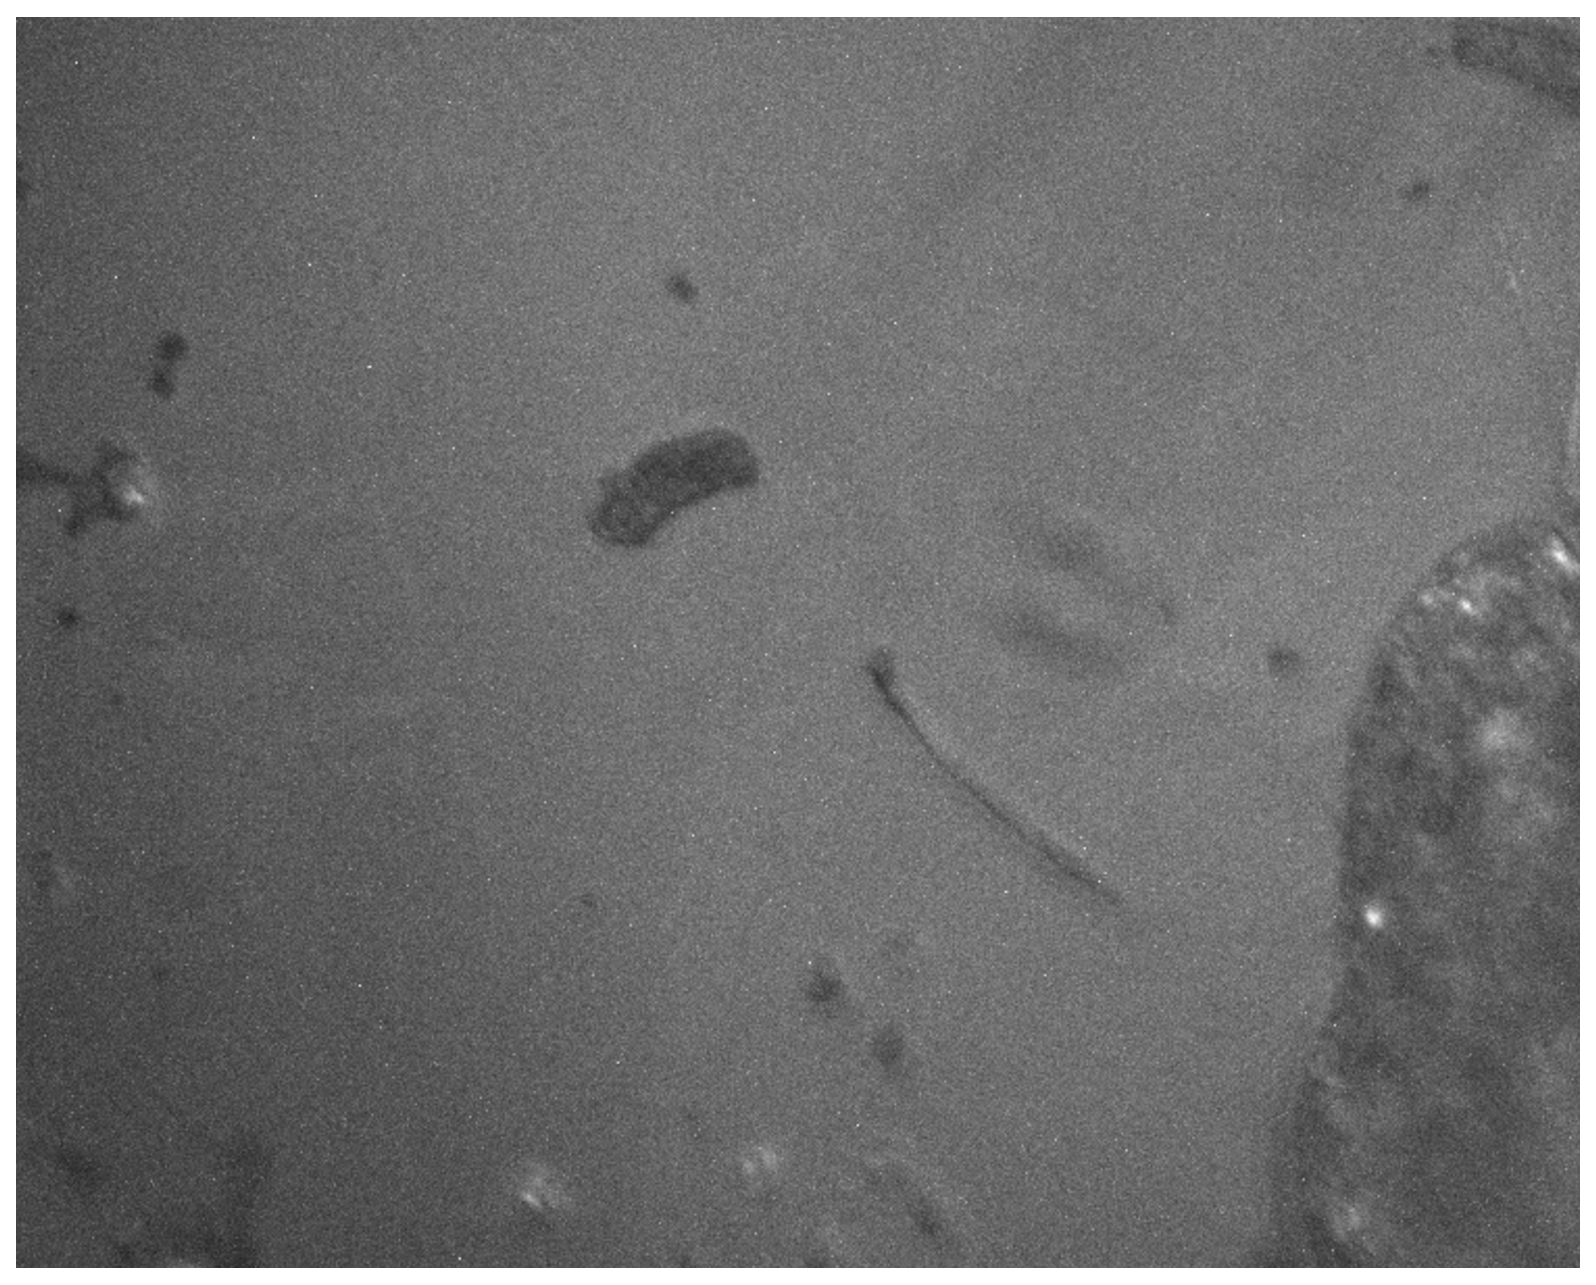
\includegraphics[width=\hsize]{vh50.eps}
  \end{center}
  \caption{直交偏光(y偏光/x検出)}
  \label{fig:vh50}
 \end{minipage}
\end{figure}

\section{光学クライオスタット}
\subsection{冷凍機}
Advenced Research Systems社の冷凍機(DE204)を用いた。

\subsection{真空引きポンプ}
ロータリーポンプとオイルポンプ

次に試料に光学軸が存在すると仮定する。さらに試料の光学軸が、顕微鏡像で細長く明るい領域が伸びる方向と平行であると仮定する。この時定性的に、上で述べたような図\ref{fig:vh250}と図\ref{fig:hv250}の反射率の変化が説明できる(できない)。直交偏光条件で、\label{sec:diagonazed_reflectance}より、入射光の偏光が試料の光学軸に平行であるか直交するとき反射率は最小である。また入射光の偏光が光学軸と角45度をなすとき信号強度は最大になる。図\ref{fig:vh250}で入射光の偏光はy方向で、画像横方向となす角が140度である。図\ref{fig:vh250}左下の光学軸の方向は画像横方向となす角が111度であり、偏光方向と相対角29度をなす。また図\ref{fig:vh250}右上の光学軸の方向は画像横方向となす角が49度であり、偏光方向と91度程度の角度をなす。一方、図\ref{fig:hv250}で入射光の偏光はx方向で、画像横方向となす角が50度である。図\ref{fig:vh250}左下の明るい領域の光学軸の方向は画像横方向となす角が111度で、偏光方向と相対角61度をなす。また図\ref{fig:vh250}右上の光学軸の方向は画像横方向となす角が49度で、偏光方向と相対角1度をなす。
\begin{table}[htb]
  \begin{tabular}{lcrr}
     & 左下 & 右上  \\
    図\ref{fig:vh250} & 29 & 91\\
    図\ref{fig:hv250} & 61 & 1
    \label{tab:入射光の偏光と試料の光学軸の相対角度}
  \end{tabular}
\end{table}
\end{comment}

\section{Optimization of the sputtering condition}
\subsection{Substrate temperature and the density of Argon gas}

Thornton 
\subsection{Thickness of tin films}
\subsection{InSb}
\subsection{Voltage to }

\bibliography{zenki_jikken.bib}
\bibliographystyle{junsrt}


\end{document}
%コンパイルの仕方
%1. texファイルを一回コンパイル
%2. bibファイルを一回コンパイル
%3. texファイルを三回コンパイル